
% Default to the notebook output style

    


% Inherit from the specified cell style.




    
\documentclass[11pt]{article}

    
    
    \usepackage[T1]{fontenc}
    % Nicer default font (+ math font) than Computer Modern for most use cases
    \usepackage{mathpazo}

    % Basic figure setup, for now with no caption control since it's done
    % automatically by Pandoc (which extracts ![](path) syntax from Markdown).
    \usepackage{graphicx}
    % We will generate all images so they have a width \maxwidth. This means
    % that they will get their normal width if they fit onto the page, but
    % are scaled down if they would overflow the margins.
    \makeatletter
    \def\maxwidth{\ifdim\Gin@nat@width>\linewidth\linewidth
    \else\Gin@nat@width\fi}
    \makeatother
    \let\Oldincludegraphics\includegraphics
    % Set max figure width to be 80% of text width, for now hardcoded.
    \renewcommand{\includegraphics}[1]{\Oldincludegraphics[width=.8\maxwidth]{#1}}
    % Ensure that by default, figures have no caption (until we provide a
    % proper Figure object with a Caption API and a way to capture that
    % in the conversion process - todo).
    \usepackage{caption}
    \DeclareCaptionLabelFormat{nolabel}{}
    \captionsetup{labelformat=nolabel}

    \usepackage{adjustbox} % Used to constrain images to a maximum size 
    \usepackage{xcolor} % Allow colors to be defined
    \usepackage{enumerate} % Needed for markdown enumerations to work
    \usepackage{geometry} % Used to adjust the document margins
    \usepackage{amsmath} % Equations
    \usepackage{amssymb} % Equations
    \usepackage{textcomp} % defines textquotesingle
    % Hack from http://tex.stackexchange.com/a/47451/13684:
    \AtBeginDocument{%
        \def\PYZsq{\textquotesingle}% Upright quotes in Pygmentized code
    }
    \usepackage{upquote} % Upright quotes for verbatim code
    \usepackage{eurosym} % defines \euro
    \usepackage[mathletters]{ucs} % Extended unicode (utf-8) support
    \usepackage[utf8x]{inputenc} % Allow utf-8 characters in the tex document
    \usepackage{fancyvrb} % verbatim replacement that allows latex
    \usepackage{grffile} % extends the file name processing of package graphics 
                         % to support a larger range 
    % The hyperref package gives us a pdf with properly built
    % internal navigation ('pdf bookmarks' for the table of contents,
    % internal cross-reference links, web links for URLs, etc.)
    \usepackage{hyperref}
    \usepackage{longtable} % longtable support required by pandoc >1.10
    \usepackage{booktabs}  % table support for pandoc > 1.12.2
    \usepackage[inline]{enumitem} % IRkernel/repr support (it uses the enumerate* environment)
    \usepackage[normalem]{ulem} % ulem is needed to support strikethroughs (\sout)
                                % normalem makes italics be italics, not underlines
    \usepackage{mathrsfs}
    

    
    
    % Colors for the hyperref package
    \definecolor{urlcolor}{rgb}{0,.145,.698}
    \definecolor{linkcolor}{rgb}{.71,0.21,0.01}
    \definecolor{citecolor}{rgb}{.12,.54,.11}

    % ANSI colors
    \definecolor{ansi-black}{HTML}{3E424D}
    \definecolor{ansi-black-intense}{HTML}{282C36}
    \definecolor{ansi-red}{HTML}{E75C58}
    \definecolor{ansi-red-intense}{HTML}{B22B31}
    \definecolor{ansi-green}{HTML}{00A250}
    \definecolor{ansi-green-intense}{HTML}{007427}
    \definecolor{ansi-yellow}{HTML}{DDB62B}
    \definecolor{ansi-yellow-intense}{HTML}{B27D12}
    \definecolor{ansi-blue}{HTML}{208FFB}
    \definecolor{ansi-blue-intense}{HTML}{0065CA}
    \definecolor{ansi-magenta}{HTML}{D160C4}
    \definecolor{ansi-magenta-intense}{HTML}{A03196}
    \definecolor{ansi-cyan}{HTML}{60C6C8}
    \definecolor{ansi-cyan-intense}{HTML}{258F8F}
    \definecolor{ansi-white}{HTML}{C5C1B4}
    \definecolor{ansi-white-intense}{HTML}{A1A6B2}
    \definecolor{ansi-default-inverse-fg}{HTML}{FFFFFF}
    \definecolor{ansi-default-inverse-bg}{HTML}{000000}

    % commands and environments needed by pandoc snippets
    % extracted from the output of `pandoc -s`
    \providecommand{\tightlist}{%
      \setlength{\itemsep}{0pt}\setlength{\parskip}{0pt}}
    \DefineVerbatimEnvironment{Highlighting}{Verbatim}{commandchars=\\\{\}}
    % Add ',fontsize=\small' for more characters per line
    \newenvironment{Shaded}{}{}
    \newcommand{\KeywordTok}[1]{\textcolor[rgb]{0.00,0.44,0.13}{\textbf{{#1}}}}
    \newcommand{\DataTypeTok}[1]{\textcolor[rgb]{0.56,0.13,0.00}{{#1}}}
    \newcommand{\DecValTok}[1]{\textcolor[rgb]{0.25,0.63,0.44}{{#1}}}
    \newcommand{\BaseNTok}[1]{\textcolor[rgb]{0.25,0.63,0.44}{{#1}}}
    \newcommand{\FloatTok}[1]{\textcolor[rgb]{0.25,0.63,0.44}{{#1}}}
    \newcommand{\CharTok}[1]{\textcolor[rgb]{0.25,0.44,0.63}{{#1}}}
    \newcommand{\StringTok}[1]{\textcolor[rgb]{0.25,0.44,0.63}{{#1}}}
    \newcommand{\CommentTok}[1]{\textcolor[rgb]{0.38,0.63,0.69}{\textit{{#1}}}}
    \newcommand{\OtherTok}[1]{\textcolor[rgb]{0.00,0.44,0.13}{{#1}}}
    \newcommand{\AlertTok}[1]{\textcolor[rgb]{1.00,0.00,0.00}{\textbf{{#1}}}}
    \newcommand{\FunctionTok}[1]{\textcolor[rgb]{0.02,0.16,0.49}{{#1}}}
    \newcommand{\RegionMarkerTok}[1]{{#1}}
    \newcommand{\ErrorTok}[1]{\textcolor[rgb]{1.00,0.00,0.00}{\textbf{{#1}}}}
    \newcommand{\NormalTok}[1]{{#1}}
    
    % Additional commands for more recent versions of Pandoc
    \newcommand{\ConstantTok}[1]{\textcolor[rgb]{0.53,0.00,0.00}{{#1}}}
    \newcommand{\SpecialCharTok}[1]{\textcolor[rgb]{0.25,0.44,0.63}{{#1}}}
    \newcommand{\VerbatimStringTok}[1]{\textcolor[rgb]{0.25,0.44,0.63}{{#1}}}
    \newcommand{\SpecialStringTok}[1]{\textcolor[rgb]{0.73,0.40,0.53}{{#1}}}
    \newcommand{\ImportTok}[1]{{#1}}
    \newcommand{\DocumentationTok}[1]{\textcolor[rgb]{0.73,0.13,0.13}{\textit{{#1}}}}
    \newcommand{\AnnotationTok}[1]{\textcolor[rgb]{0.38,0.63,0.69}{\textbf{\textit{{#1}}}}}
    \newcommand{\CommentVarTok}[1]{\textcolor[rgb]{0.38,0.63,0.69}{\textbf{\textit{{#1}}}}}
    \newcommand{\VariableTok}[1]{\textcolor[rgb]{0.10,0.09,0.49}{{#1}}}
    \newcommand{\ControlFlowTok}[1]{\textcolor[rgb]{0.00,0.44,0.13}{\textbf{{#1}}}}
    \newcommand{\OperatorTok}[1]{\textcolor[rgb]{0.40,0.40,0.40}{{#1}}}
    \newcommand{\BuiltInTok}[1]{{#1}}
    \newcommand{\ExtensionTok}[1]{{#1}}
    \newcommand{\PreprocessorTok}[1]{\textcolor[rgb]{0.74,0.48,0.00}{{#1}}}
    \newcommand{\AttributeTok}[1]{\textcolor[rgb]{0.49,0.56,0.16}{{#1}}}
    \newcommand{\InformationTok}[1]{\textcolor[rgb]{0.38,0.63,0.69}{\textbf{\textit{{#1}}}}}
    \newcommand{\WarningTok}[1]{\textcolor[rgb]{0.38,0.63,0.69}{\textbf{\textit{{#1}}}}}
    
    
    % Define a nice break command that doesn't care if a line doesn't already
    % exist.
    \def\br{\hspace*{\fill} \\* }
    % Math Jax compatibility definitions
    \def\gt{>}
    \def\lt{<}
    \let\Oldtex\TeX
    \let\Oldlatex\LaTeX
    \renewcommand{\TeX}{\textrm{\Oldtex}}
    \renewcommand{\LaTeX}{\textrm{\Oldlatex}}
    % Document parameters
    % Document title
    \title{Learning Decision-Making patterns in the OFC\\[1em]
    \large An analysis of a gambling task on epileptic patientst}
    \author{Nader Namini Asl\\[0.75em]\small CogSci C127 Fall 2018}
    
    
    
    

    % Pygments definitions
    
\makeatletter
\def\PY@reset{\let\PY@it=\relax \let\PY@bf=\relax%
    \let\PY@ul=\relax \let\PY@tc=\relax%
    \let\PY@bc=\relax \let\PY@ff=\relax}
\def\PY@tok#1{\csname PY@tok@#1\endcsname}
\def\PY@toks#1+{\ifx\relax#1\empty\else%
    \PY@tok{#1}\expandafter\PY@toks\fi}
\def\PY@do#1{\PY@bc{\PY@tc{\PY@ul{%
    \PY@it{\PY@bf{\PY@ff{#1}}}}}}}
\def\PY#1#2{\PY@reset\PY@toks#1+\relax+\PY@do{#2}}

\expandafter\def\csname PY@tok@w\endcsname{\def\PY@tc##1{\textcolor[rgb]{0.73,0.73,0.73}{##1}}}
\expandafter\def\csname PY@tok@c\endcsname{\let\PY@it=\textit\def\PY@tc##1{\textcolor[rgb]{0.25,0.50,0.50}{##1}}}
\expandafter\def\csname PY@tok@cp\endcsname{\def\PY@tc##1{\textcolor[rgb]{0.74,0.48,0.00}{##1}}}
\expandafter\def\csname PY@tok@k\endcsname{\let\PY@bf=\textbf\def\PY@tc##1{\textcolor[rgb]{0.00,0.50,0.00}{##1}}}
\expandafter\def\csname PY@tok@kp\endcsname{\def\PY@tc##1{\textcolor[rgb]{0.00,0.50,0.00}{##1}}}
\expandafter\def\csname PY@tok@kt\endcsname{\def\PY@tc##1{\textcolor[rgb]{0.69,0.00,0.25}{##1}}}
\expandafter\def\csname PY@tok@o\endcsname{\def\PY@tc##1{\textcolor[rgb]{0.40,0.40,0.40}{##1}}}
\expandafter\def\csname PY@tok@ow\endcsname{\let\PY@bf=\textbf\def\PY@tc##1{\textcolor[rgb]{0.67,0.13,1.00}{##1}}}
\expandafter\def\csname PY@tok@nb\endcsname{\def\PY@tc##1{\textcolor[rgb]{0.00,0.50,0.00}{##1}}}
\expandafter\def\csname PY@tok@nf\endcsname{\def\PY@tc##1{\textcolor[rgb]{0.00,0.00,1.00}{##1}}}
\expandafter\def\csname PY@tok@nc\endcsname{\let\PY@bf=\textbf\def\PY@tc##1{\textcolor[rgb]{0.00,0.00,1.00}{##1}}}
\expandafter\def\csname PY@tok@nn\endcsname{\let\PY@bf=\textbf\def\PY@tc##1{\textcolor[rgb]{0.00,0.00,1.00}{##1}}}
\expandafter\def\csname PY@tok@ne\endcsname{\let\PY@bf=\textbf\def\PY@tc##1{\textcolor[rgb]{0.82,0.25,0.23}{##1}}}
\expandafter\def\csname PY@tok@nv\endcsname{\def\PY@tc##1{\textcolor[rgb]{0.10,0.09,0.49}{##1}}}
\expandafter\def\csname PY@tok@no\endcsname{\def\PY@tc##1{\textcolor[rgb]{0.53,0.00,0.00}{##1}}}
\expandafter\def\csname PY@tok@nl\endcsname{\def\PY@tc##1{\textcolor[rgb]{0.63,0.63,0.00}{##1}}}
\expandafter\def\csname PY@tok@ni\endcsname{\let\PY@bf=\textbf\def\PY@tc##1{\textcolor[rgb]{0.60,0.60,0.60}{##1}}}
\expandafter\def\csname PY@tok@na\endcsname{\def\PY@tc##1{\textcolor[rgb]{0.49,0.56,0.16}{##1}}}
\expandafter\def\csname PY@tok@nt\endcsname{\let\PY@bf=\textbf\def\PY@tc##1{\textcolor[rgb]{0.00,0.50,0.00}{##1}}}
\expandafter\def\csname PY@tok@nd\endcsname{\def\PY@tc##1{\textcolor[rgb]{0.67,0.13,1.00}{##1}}}
\expandafter\def\csname PY@tok@s\endcsname{\def\PY@tc##1{\textcolor[rgb]{0.73,0.13,0.13}{##1}}}
\expandafter\def\csname PY@tok@sd\endcsname{\let\PY@it=\textit\def\PY@tc##1{\textcolor[rgb]{0.73,0.13,0.13}{##1}}}
\expandafter\def\csname PY@tok@si\endcsname{\let\PY@bf=\textbf\def\PY@tc##1{\textcolor[rgb]{0.73,0.40,0.53}{##1}}}
\expandafter\def\csname PY@tok@se\endcsname{\let\PY@bf=\textbf\def\PY@tc##1{\textcolor[rgb]{0.73,0.40,0.13}{##1}}}
\expandafter\def\csname PY@tok@sr\endcsname{\def\PY@tc##1{\textcolor[rgb]{0.73,0.40,0.53}{##1}}}
\expandafter\def\csname PY@tok@ss\endcsname{\def\PY@tc##1{\textcolor[rgb]{0.10,0.09,0.49}{##1}}}
\expandafter\def\csname PY@tok@sx\endcsname{\def\PY@tc##1{\textcolor[rgb]{0.00,0.50,0.00}{##1}}}
\expandafter\def\csname PY@tok@m\endcsname{\def\PY@tc##1{\textcolor[rgb]{0.40,0.40,0.40}{##1}}}
\expandafter\def\csname PY@tok@gh\endcsname{\let\PY@bf=\textbf\def\PY@tc##1{\textcolor[rgb]{0.00,0.00,0.50}{##1}}}
\expandafter\def\csname PY@tok@gu\endcsname{\let\PY@bf=\textbf\def\PY@tc##1{\textcolor[rgb]{0.50,0.00,0.50}{##1}}}
\expandafter\def\csname PY@tok@gd\endcsname{\def\PY@tc##1{\textcolor[rgb]{0.63,0.00,0.00}{##1}}}
\expandafter\def\csname PY@tok@gi\endcsname{\def\PY@tc##1{\textcolor[rgb]{0.00,0.63,0.00}{##1}}}
\expandafter\def\csname PY@tok@gr\endcsname{\def\PY@tc##1{\textcolor[rgb]{1.00,0.00,0.00}{##1}}}
\expandafter\def\csname PY@tok@ge\endcsname{\let\PY@it=\textit}
\expandafter\def\csname PY@tok@gs\endcsname{\let\PY@bf=\textbf}
\expandafter\def\csname PY@tok@gp\endcsname{\let\PY@bf=\textbf\def\PY@tc##1{\textcolor[rgb]{0.00,0.00,0.50}{##1}}}
\expandafter\def\csname PY@tok@go\endcsname{\def\PY@tc##1{\textcolor[rgb]{0.53,0.53,0.53}{##1}}}
\expandafter\def\csname PY@tok@gt\endcsname{\def\PY@tc##1{\textcolor[rgb]{0.00,0.27,0.87}{##1}}}
\expandafter\def\csname PY@tok@err\endcsname{\def\PY@bc##1{\setlength{\fboxsep}{0pt}\fcolorbox[rgb]{1.00,0.00,0.00}{1,1,1}{\strut ##1}}}
\expandafter\def\csname PY@tok@kc\endcsname{\let\PY@bf=\textbf\def\PY@tc##1{\textcolor[rgb]{0.00,0.50,0.00}{##1}}}
\expandafter\def\csname PY@tok@kd\endcsname{\let\PY@bf=\textbf\def\PY@tc##1{\textcolor[rgb]{0.00,0.50,0.00}{##1}}}
\expandafter\def\csname PY@tok@kn\endcsname{\let\PY@bf=\textbf\def\PY@tc##1{\textcolor[rgb]{0.00,0.50,0.00}{##1}}}
\expandafter\def\csname PY@tok@kr\endcsname{\let\PY@bf=\textbf\def\PY@tc##1{\textcolor[rgb]{0.00,0.50,0.00}{##1}}}
\expandafter\def\csname PY@tok@bp\endcsname{\def\PY@tc##1{\textcolor[rgb]{0.00,0.50,0.00}{##1}}}
\expandafter\def\csname PY@tok@fm\endcsname{\def\PY@tc##1{\textcolor[rgb]{0.00,0.00,1.00}{##1}}}
\expandafter\def\csname PY@tok@vc\endcsname{\def\PY@tc##1{\textcolor[rgb]{0.10,0.09,0.49}{##1}}}
\expandafter\def\csname PY@tok@vg\endcsname{\def\PY@tc##1{\textcolor[rgb]{0.10,0.09,0.49}{##1}}}
\expandafter\def\csname PY@tok@vi\endcsname{\def\PY@tc##1{\textcolor[rgb]{0.10,0.09,0.49}{##1}}}
\expandafter\def\csname PY@tok@vm\endcsname{\def\PY@tc##1{\textcolor[rgb]{0.10,0.09,0.49}{##1}}}
\expandafter\def\csname PY@tok@sa\endcsname{\def\PY@tc##1{\textcolor[rgb]{0.73,0.13,0.13}{##1}}}
\expandafter\def\csname PY@tok@sb\endcsname{\def\PY@tc##1{\textcolor[rgb]{0.73,0.13,0.13}{##1}}}
\expandafter\def\csname PY@tok@sc\endcsname{\def\PY@tc##1{\textcolor[rgb]{0.73,0.13,0.13}{##1}}}
\expandafter\def\csname PY@tok@dl\endcsname{\def\PY@tc##1{\textcolor[rgb]{0.73,0.13,0.13}{##1}}}
\expandafter\def\csname PY@tok@s2\endcsname{\def\PY@tc##1{\textcolor[rgb]{0.73,0.13,0.13}{##1}}}
\expandafter\def\csname PY@tok@sh\endcsname{\def\PY@tc##1{\textcolor[rgb]{0.73,0.13,0.13}{##1}}}
\expandafter\def\csname PY@tok@s1\endcsname{\def\PY@tc##1{\textcolor[rgb]{0.73,0.13,0.13}{##1}}}
\expandafter\def\csname PY@tok@mb\endcsname{\def\PY@tc##1{\textcolor[rgb]{0.40,0.40,0.40}{##1}}}
\expandafter\def\csname PY@tok@mf\endcsname{\def\PY@tc##1{\textcolor[rgb]{0.40,0.40,0.40}{##1}}}
\expandafter\def\csname PY@tok@mh\endcsname{\def\PY@tc##1{\textcolor[rgb]{0.40,0.40,0.40}{##1}}}
\expandafter\def\csname PY@tok@mi\endcsname{\def\PY@tc##1{\textcolor[rgb]{0.40,0.40,0.40}{##1}}}
\expandafter\def\csname PY@tok@il\endcsname{\def\PY@tc##1{\textcolor[rgb]{0.40,0.40,0.40}{##1}}}
\expandafter\def\csname PY@tok@mo\endcsname{\def\PY@tc##1{\textcolor[rgb]{0.40,0.40,0.40}{##1}}}
\expandafter\def\csname PY@tok@ch\endcsname{\let\PY@it=\textit\def\PY@tc##1{\textcolor[rgb]{0.25,0.50,0.50}{##1}}}
\expandafter\def\csname PY@tok@cm\endcsname{\let\PY@it=\textit\def\PY@tc##1{\textcolor[rgb]{0.25,0.50,0.50}{##1}}}
\expandafter\def\csname PY@tok@cpf\endcsname{\let\PY@it=\textit\def\PY@tc##1{\textcolor[rgb]{0.25,0.50,0.50}{##1}}}
\expandafter\def\csname PY@tok@c1\endcsname{\let\PY@it=\textit\def\PY@tc##1{\textcolor[rgb]{0.25,0.50,0.50}{##1}}}
\expandafter\def\csname PY@tok@cs\endcsname{\let\PY@it=\textit\def\PY@tc##1{\textcolor[rgb]{0.25,0.50,0.50}{##1}}}

\def\PYZbs{\char`\\}
\def\PYZus{\char`\_}
\def\PYZob{\char`\{}
\def\PYZcb{\char`\}}
\def\PYZca{\char`\^}
\def\PYZam{\char`\&}
\def\PYZlt{\char`\<}
\def\PYZgt{\char`\>}
\def\PYZsh{\char`\#}
\def\PYZpc{\char`\%}
\def\PYZdl{\char`\$}
\def\PYZhy{\char`\-}
\def\PYZsq{\char`\'}
\def\PYZdq{\char`\"}
\def\PYZti{\char`\~}
% for compatibility with earlier versions
\def\PYZat{@}
\def\PYZlb{[}
\def\PYZrb{]}
\makeatother


    % Exact colors from NB
    \definecolor{incolor}{rgb}{0.0, 0.0, 0.5}
    \definecolor{outcolor}{rgb}{0.545, 0.0, 0.0}



    
    % Prevent overflowing lines due to hard-to-break entities
    \sloppy 
    % Setup hyperref package
    \hypersetup{
      breaklinks=true,  % so long urls are correctly broken across lines
      colorlinks=true,
      urlcolor=urlcolor,
      linkcolor=linkcolor,
      citecolor=citecolor,
      }
    % Slightly bigger margins than the latex defaults
    
    \geometry{verbose,tmargin=1in,bmargin=1in,lmargin=1in,rmargin=1in}
    
    

    \begin{document}
    
    
    \maketitle
    
    
\section{}

    \hypertarget{introduction-i.e.background-and-significance}{%
\subsection{Introduction (i.e.~Background and
Significance)}\label{introduction-i.e.background-and-significance}}

    \textbf{Research question:} ``Can we use a machine learning
classification model to predict decisions based on neural activity in
the orbito-frontal cortex? The answer to this question would allow us,
by looking at the learned model, to better understand how patterns of
neural activity can lead to a decision.''

This notebook is going to explore the possibility of using a machine
learning model, such as convolutional neural networks, to predict an
individual's decisions based on neural activity in the orbito-frontal
cortex (OFC). There have been numerous studies and experiments on the
role of OFC in human decision making. In one study, it was found that
the activity in the OFC is reduced if the individual is told what to do
as opposed to when the individual is free to make his or her choice
{[}7{]}. It was further found that the neurons in the frontal cortex,
which includes the OFC, encoded both the predicted outcome during the
choice phase of a decision-making task as well as the experienced
outcome in the outcome phase of the same task {[}5{]}. Experiments on
this topic also try to learn from the cross-species differences and
similarities in the OFC {[}6{]}. Most of these studies point to the main
role that the OFC plays in processing rewards by integrating multiple
sources of information regarding reward outcome to derive a value signal
{[}2{]}{[}3{]}. Moreover, OFC has been implicated in an individual's
understanding of the level of ambiguity and risk in a decision-making
task {[}9{]}. These findings illustrate the importance of OFC in the
decision-making process in humans. Our goal is to take a different
approach to these studies and try to produce a computational model that
is able to learn the activity patterns of OFC and be able to accurately
produce outcomes (i.e., predictions) that match the one's produced by
the individual with those activity patterns. This computational model
coupled with an understanding of what it represents and encodes can
significantly aid our understanding of the human decision-making
process.

The importance of having a model of the decision-making process is
exhaustively explored in a paper by Rangel, et al. {[}8{]}. One of the
main uses of this understanding is in psychiatry, as explored in an fMRI
study of young patients with major depressive disorder (MDD), who
exhibited less neural response than control participants, i.e., young
patients with no history of psychiatric disorders, in reward-related
brain areas, including the OFC, during both the decision/anticipation
and outcome phase of a reward decision-making task {[}4{]}. It can,
also, aid in understanding the underlying causes of neuropsychiatric and
behavioral disorders associated with diminished neural sensitivity to
losses among individuals {[}10{]}{[}11{]} as well as provide better
support for individuals suffering from substance abuse, such as cocaine
abuse, who show persistent functional abnormalities in the prefrontal
neural networks involved in decision-making {[}1{]}. In this notebook,
we will solely focus on the role of OFC as the dataset is limited to the
recordings in this area, but it should be noted that the decision-making
network in the human brain consists of the various functional areas,
including but not limited to the OFC, anterior cingulate cortex (ACC),
dorsolateral prefrontal cortex (DLPFC), and the dorsal anterior
cingulate cortices (ACd). Moreover, recently, it has been shown that the
emotional processes, mainly those associated wtih the amygdala, can
influence the human decision {[}12{]}. Therefore, to develop a
comprehensive model of the decision-making network in the brain, all
these areas need to be considered and included in the model.
Nevertheless, a computational model of the OFC and decisions can provide
a foundational step towards this comprehensive model as the OFC plays a
pivotal role in how humans make decisions.

Note, for a general case, the problem of finding a classification
algorithm to predict a decision is unbounded as the number of possible
outcomes are infinite, so we focused on a binary classification case, as
described in the \textbf{Data analysis and Results} section.

    \hypertarget{methods-and-dataset-description}{%
\subsection{Methods and dataset
description}\label{methods-and-dataset-description}}

    For this project, I am using the
\href{http://crcns.org/data-sets/ofc/ofc-3/about-ofc-2}{ofc-3 dataset}1.
This dataset contains electrocorticography (ECoG) recordings from the
orbitofrontal cortex (OFC) of n=10 neurosurgical patients being operated
on for the treatment of epilepsy. During the ECoG recordings, patients
played a simple decision-making task (a gambling game) -- the behavior
and timestamps of the relevant events were recorded. Recordings last
\textasciitilde{}15min on average, each including 200 behavioral trials.
The following description of the dataset has been inspired by the
dataset description found
\href{http://crcns.org/files/data/ofc-3/crcns_ofc-3_data_description.pdf}{here}:
\#\#\#\# Subjects Data was collected from 10 (4 female) adult subjects
with intractable epilepsy who were implanted with chronic subdural grid
and/or strip electrodes as part of a preoperative procedure to localize
the epileptogenic focus. We paid careful attention to the patient's
neurological condition and only tested when the patient was fully alert
and cooperative. The surgeons determined electrode placement and
treatment based solely on the clinical needs of each patient. Due to IRB
limitations, subjects were not paid for their participation in the study
but were encouraged to make as many points as possible. As part of the
clinical observation procedure, patients were off anti-epileptic
medication during these experiments. All subjects gave written informed
consent to participate in the study in accordance with the University of
California, Berkeley Institutional Review Board. \#\#\#\# Behavioral
Task

We probed risk-reward tradeoffs using a simple gambling task in which
subjects chose between a sure payoff and a gamble for potential higher
winnings. Trials started with a fixation cross (t=0), followed by the
game presentation screen (t=750ms). At that time, patients were given up
to 2s to choose between a fixed prize (safe bet, 10 dollars) and a
higher payoff (e.g.~30 dollars). Gamble prizes varied between 10 and 30
dollars, in 5-dollar increments. If the patient did not choose within
the allotted time limit, a timeout occurred and no reward was awarded
for that round. Timeouts were infrequent (9.98\% of all trials) and were
excluded from analysis. Gamble win probability varied round by round; at
the time of game presentation, subjects are shown a number between 0-10.
At the time of outcome (t=550ms post-choice), a second number (also 0-
10) is revealed, and the subject wins the prize if the second number is
greater than the first one. Only integers were presented, and ties were
not allowed; therefore, a shown `2' had a win probability of 20\%. The
delay between buttonpress and gamble outcome presentation (550ms) was
fixed, and activity for both epochs is temporally aligned. Therefore,
offer value, risk and chosen value vary parametrically on a
round-by-round basis, and patients had full knowledge of the (fair) task
structure from the beginning of the game. Both numbers were randomly
generated using a uniform distribution. The gamble outcome (win/loss)
was revealed regardless of subject choice, allowing us to calculate
experiential and counterfactual prediction errors (see Behavioral
analysis, below). A new round started 1s after outcome reveal. Patients
played a total of 200 rounds (plus practice rounds), and a full
experimental run typically lasted 12-15min. Location of safe bet and
gamble options (left/right) was randomized across trials. Patients
completed a training session prior to the game in which they played at
least 10 rounds under the experimenter's supervision until they felt
confident they understood the task, at which point they started the
game. This gambling task minimized other cognitive demands (working
memory, learning, etc.) on our participants, while at the same time
allowing us to probe important decision-making components implicated in
previous computational and empirical studies,

\hypertarget{ecog-recording}{%
\paragraph{ECoG Recording}\label{ecog-recording}}

ECoG has a sptial resolutions of \textasciitilde{}1cm and a temporal
resolution of smaller than 5ms {[}1{]}. The recorded data is in 2D but
it directly measuresneural activity and has a relatively good signal
quality. ECoG was recorded and stored with behavioral data. Data
processing was: channels were amplified x10000, analog filtered
(0.01-1000 Hz) with \textgreater{}2kHz digitization rate, re-referenced
to a common average off-line, high-pass filtered at 1.0 Hz with a
symmetrical (phase true) finite impulse response (FIR) filter
(\textasciitilde{}35 dB/octave roll-off). Channels with low
signal-to-noise ratio (SNR) were identified and deleted (i.e.~60 Hz line
interference, electromagnetic equipment noise, amplifier saturation,
poor contact with cortical surface). Out of 210 OFC electrodes, 192 were
artifact-free and included in subsequent analyses and in the current
dataset. Additionally, all channels were visually inspected by a
neurologist to exclude epochs of aberrant or noisy activity (typically
\textless{}1\% of datapoints). A photodiode recorded screen updates in
the behavioral task, recorded in the electrophysiological system as an
analog input and used to synchronize behavioral and electrophysiological
data. Data analysis was carried out in MATLAB and R using custom
scripts. Data for each channel was downsampled to 1KHz and filtered into
high frequency activity (HFA; 70--200 Hz) using a two-way, zero
phase-lag, finite impulse response band pass filter to prevent phase
distortion.

1 Originally, this project was going to utilize the
\href{http://crcns.org/data-sets/ofc/ofc-1/about-ofc-1}{ofc-1} and
\href{http://crcns.org/data-sets/ofc/ofc-2/about-ofc-2}{ofc-2} datasets
which contain the recordings from orbitofrontal cortex of five and three
rats during an odor discrimination task, respectively. However, since
the project limited its scope to human participants, we have decided to
exclude those datasets from the current project, even though they could
be used in a similar cross-species data analysis project.

    \hypertarget{data-analysis-and-results}{%
\subsection{Data analysis and Results}\label{data-analysis-and-results}}

    Initially, the PCA and ICA were intended to be used for reducing the
dimensionality of the ECoG signal data from this dataset. However, upon
closer inspection for data for each subject, since recordings only take
place for a few hundred miliseconds across a handful (on average
\textasciitilde{}10) of electrodes, it was decided that dimensionality
reduction would not be needed. Therefore, in the following sections, we
will, first, start with analyzing the ECoG recording data and then using
each of the following methods to try to find a classification model
(according to the research question) that is able to predict each
subject's decision. It should be noted that a separate model (for each
of the algorithms below) was trained and test for each subject due to
the significant individual differences between the individiuals in this
datasets: subjects suffer from intractable epilepsy and each have a
varying number of electrodes implanted during their operation. -
\emph{Fully-connected Neural Network} - \emph{Convolutional Neural
Network} - \emph{Decision Trees} - \emph{Decision Tree Classifier} -
\emph{Decision Tree Ensembles} - \emph{Random Forest} - \emph{AdaBoost}

    \hypertarget{data-preprocessing}{%
\subsubsection{Data preprocessing}\label{data-preprocessing}}

    \hypertarget{imports}{%
\paragraph{Imports}\label{imports}}

    \begin{Verbatim}[commandchars=\\\{\}]
{\color{incolor}In [{\color{incolor}137}]:} \PY{k+kn}{from} \PY{n+nn}{utils} \PY{k}{import} \PY{n}{get\PYZus{}data}\PY{p}{,} \PY{n}{delete\PYZus{}files\PYZus{}in\PYZus{}folder}
          \PY{k+kn}{import} \PY{n+nn}{matplotlib}\PY{n+nn}{.}\PY{n+nn}{pyplot} \PY{k}{as} \PY{n+nn}{plt}
          \PY{k+kn}{import} \PY{n+nn}{matplotlib}\PY{n+nn}{.}\PY{n+nn}{cm} \PY{k}{as} \PY{n+nn}{cm}
          \PY{c+c1}{\PYZsh{} utility functions}
          \PY{k+kn}{from} \PY{n+nn}{mpl\PYZus{}toolkits}\PY{n+nn}{.}\PY{n+nn}{axes\PYZus{}grid1} \PY{k}{import} \PY{n}{make\PYZus{}axes\PYZus{}locatable}
          \PY{c+c1}{\PYZsh{} TensorFlow and tf.keras}
          \PY{k+kn}{import} \PY{n+nn}{tensorflow} \PY{k}{as} \PY{n+nn}{tf}
          \PY{k+kn}{from} \PY{n+nn}{tensorflow} \PY{k}{import} \PY{n}{keras}
          \PY{k+kn}{import} \PY{n+nn}{tensorflow}\PY{n+nn}{.}\PY{n+nn}{contrib}\PY{n+nn}{.}\PY{n+nn}{eager} \PY{k}{as} \PY{n+nn}{tfe}
          \PY{k+kn}{import} \PY{n+nn}{tensorflow}\PY{n+nn}{.}\PY{n+nn}{contrib}\PY{n+nn}{.}\PY{n+nn}{slim} \PY{k}{as} \PY{n+nn}{slim}
          \PY{n}{tf}\PY{o}{.}\PY{n}{enable\PYZus{}eager\PYZus{}execution}\PY{p}{(}\PY{p}{)}
          \PY{k+kn}{from} \PY{n+nn}{sklearn}\PY{n+nn}{.}\PY{n+nn}{model\PYZus{}selection} \PY{k}{import} \PY{n}{KFold}\PY{p}{,} \PY{n}{train\PYZus{}test\PYZus{}split}
          \PY{k+kn}{import} \PY{n+nn}{numpy} \PY{k}{as} \PY{n+nn}{np}
          \PY{k+kn}{import} \PY{n+nn}{math}
          \PY{k+kn}{import} \PY{n+nn}{warnings}
          \PY{k+kn}{import} \PY{n+nn}{pandas} \PY{k}{as} \PY{n+nn}{pd}
          \PY{n}{pd}\PY{o}{.}\PY{n}{options}\PY{o}{.}\PY{n}{mode}\PY{o}{.}\PY{n}{chained\PYZus{}assignment} \PY{o}{=} \PY{k+kc}{None}  \PY{c+c1}{\PYZsh{} default=\PYZsq{}warn\PYZsq{}}
          \PY{n}{warnings}\PY{o}{.}\PY{n}{filterwarnings}\PY{p}{(}\PY{n}{action}\PY{o}{=}\PY{l+s+s1}{\PYZsq{}}\PY{l+s+s1}{once}\PY{l+s+s1}{\PYZsq{}}\PY{p}{)}
\end{Verbatim}

    \hypertarget{data-processing}{%
\paragraph{Data Processing}\label{data-processing}}

    \begin{Verbatim}[commandchars=\\\{\}]
{\color{incolor}In [{\color{incolor}2}]:} \PY{n}{dataset} \PY{o}{=} \PY{n}{get\PYZus{}data}\PY{p}{(}\PY{l+s+s1}{\PYZsq{}}\PY{l+s+s1}{ofc\PYZhy{}3}\PY{l+s+s1}{\PYZsq{}}\PY{p}{)}
\end{Verbatim}

    \begin{Verbatim}[commandchars=\\\{\}]
{\color{incolor}In [{\color{incolor}3}]:} \PY{c+c1}{\PYZsh{} Behavioral data}
        \PY{n}{data\PYZus{}behav} \PY{o}{=} \PY{n}{dataset}\PY{p}{[}\PY{l+s+s1}{\PYZsq{}}\PY{l+s+s1}{data\PYZus{}behav}\PY{l+s+s1}{\PYZsq{}}\PY{p}{]}
        \PY{c+c1}{\PYZsh{} Electrophysiological data}
        \PY{n}{data\PYZus{}ephys} \PY{o}{=} \PY{n}{dataset}\PY{p}{[}\PY{l+s+s1}{\PYZsq{}}\PY{l+s+s1}{data\PYZus{}ephys}\PY{l+s+s1}{\PYZsq{}}\PY{p}{]}
\end{Verbatim}

    \begin{Verbatim}[commandchars=\\\{\}]
{\color{incolor}In [{\color{incolor}4}]:} \PY{c+c1}{\PYZsh{} Gamble Choices Description File}
        \PY{n}{gamble\PYZus{}choices} \PY{o}{=} \PY{n}{data\PYZus{}behav}\PY{p}{[}\PY{l+s+s1}{\PYZsq{}}\PY{l+s+s1}{gamble\PYZus{}choices.csv}\PY{l+s+s1}{\PYZsq{}}\PY{p}{]}
        \PY{c+c1}{\PYZsh{} Behavioral data for each subject}
        \PY{n}{subjects\PYZus{}behav} \PY{o}{=} \PY{p}{\PYZob{}}\PY{n}{filename}\PY{o}{.}\PY{n}{split}\PY{p}{(}\PY{l+s+s1}{\PYZsq{}}\PY{l+s+s1}{.}\PY{l+s+s1}{\PYZsq{}}\PY{p}{)}\PY{p}{[}\PY{o}{\PYZhy{}}\PY{l+m+mi}{2}\PY{p}{]}\PY{p}{:} \PY{n}{data\PYZus{}behav}\PY{p}{[}\PY{n}{filename}\PY{p}{]} \PY{k}{for} \PY{n}{filename} \PY{o+ow}{in}
                          \PY{n}{data\PYZus{}behav} \PY{k}{if} \PY{n}{filename} \PY{o}{!=} \PY{l+s+s1}{\PYZsq{}}\PY{l+s+s1}{gamble\PYZus{}choices.csv}\PY{l+s+s1}{\PYZsq{}}\PY{p}{\PYZcb{}}
        \PY{c+c1}{\PYZsh{} Electrophysiological data for each subject}
        \PY{n}{subjects\PYZus{}ephys} \PY{o}{=} \PY{p}{\PYZob{}}\PY{n}{filename}\PY{o}{.}\PY{n}{split}\PY{p}{(}\PY{l+s+s1}{\PYZsq{}}\PY{l+s+s1}{\PYZus{}}\PY{l+s+s1}{\PYZsq{}}\PY{p}{)}\PY{p}{[}\PY{l+m+mi}{0}\PY{p}{]}\PY{p}{:} \PY{n}{data\PYZus{}ephys}\PY{p}{[}\PY{n}{filename}\PY{p}{]} \PY{k}{for} \PY{n}{filename} \PY{o+ow}{in} \PY{n}{data\PYZus{}ephys}\PY{p}{\PYZcb{}}
\end{Verbatim}

    \begin{Verbatim}[commandchars=\\\{\}]
{\color{incolor}In [{\color{incolor}202}]:} \PY{n}{subject} \PY{o}{=} \PY{l+m+mi}{1}
          \PY{n}{rnd} \PY{o}{=} \PY{l+m+mi}{1}
          \PY{n}{num\PYZus{}electrodes} \PY{o}{=} \PY{n}{subjects\PYZus{}ephys}\PY{p}{[}\PY{l+s+s1}{\PYZsq{}}\PY{l+s+s1}{s}\PY{l+s+s1}{\PYZsq{}} \PY{o}{+} \PY{p}{(}\PY{l+m+mi}{2} \PY{o}{\PYZhy{}} \PY{n+nb}{len}\PY{p}{(}\PY{n+nb}{str}\PY{p}{(}\PY{n}{subject}\PY{p}{)}\PY{p}{)}\PY{p}{)} \PY{o}{*} \PY{l+s+s1}{\PYZsq{}}\PY{l+s+s1}{0}\PY{l+s+s1}{\PYZsq{}} \PY{o}{+}
                                          \PY{n+nb}{str}\PY{p}{(}\PY{n}{subject}\PY{p}{)}\PY{p}{]}\PY{p}{[}\PY{l+s+s1}{\PYZsq{}}\PY{l+s+s1}{game\PYZus{}events\PYZus{}hg}\PY{l+s+s1}{\PYZsq{}}\PY{p}{]}\PY{p}{[}\PY{n}{rnd} \PY{o}{\PYZhy{}} \PY{l+m+mi}{1}\PY{p}{]}\PY{o}{.}\PY{n}{shape}\PY{p}{[}\PY{l+m+mi}{1}\PY{p}{]}
          \PY{n+nb}{print}\PY{p}{(}\PY{n}{f}\PY{l+s+s1}{\PYZsq{}}\PY{l+s+s1}{High\PYZhy{}gamma activity at [\PYZhy{}1,2]s around round }\PY{l+s+si}{\PYZob{}rnd\PYZcb{}}\PY{l+s+se}{\PYZbs{}\PYZsq{}}\PY{l+s+s1}{s game presentation across}\PY{l+s+s1}{\PYZsq{}} \PY{o}{+}
                \PY{n}{f}\PY{l+s+s1}{\PYZsq{}}\PY{l+s+s1}{ all}\PY{l+s+se}{\PYZbs{}n}\PY{l+s+s1}{ (}\PY{l+s+si}{\PYZob{}num\PYZus{}electrodes\PYZcb{}}\PY{l+s+s1}{) electrodes for subject }\PY{l+s+si}{\PYZob{}subject\PYZcb{}}\PY{l+s+s1}{*}\PY{l+s+s1}{\PYZsq{}}\PY{p}{)}
          \PY{n+nb}{print}\PY{p}{(}\PY{l+s+s1}{\PYZsq{}}\PY{l+s+s1}{*5 randomly selected timepoints}\PY{l+s+s1}{\PYZsq{}}\PY{p}{)}
          \PY{n}{subj\PYZus{}data} \PY{o}{=} \PY{n}{subjects\PYZus{}ephys}\PY{p}{[}\PY{l+s+s1}{\PYZsq{}}\PY{l+s+s1}{s}\PY{l+s+s1}{\PYZsq{}} \PY{o}{+} \PY{p}{(}\PY{l+m+mi}{2} \PY{o}{\PYZhy{}} \PY{n+nb}{len}\PY{p}{(}\PY{n+nb}{str}\PY{p}{(}\PY{n}{subject}\PY{p}{)}\PY{p}{)}\PY{p}{)} \PY{o}{*} \PY{l+s+s1}{\PYZsq{}}\PY{l+s+s1}{0}\PY{l+s+s1}{\PYZsq{}}
                                     \PY{o}{+} \PY{n+nb}{str}\PY{p}{(}\PY{n}{subject}\PY{p}{)}\PY{p}{]}\PY{p}{[}\PY{l+s+s1}{\PYZsq{}}\PY{l+s+s1}{game\PYZus{}events\PYZus{}hg}\PY{l+s+s1}{\PYZsq{}}\PY{p}{]}\PY{p}{[}\PY{n}{rnd} \PY{o}{\PYZhy{}} \PY{l+m+mi}{1}\PY{p}{]}
          \PY{n+nb}{print}\PY{p}{(}\PY{n}{subj\PYZus{}data}\PY{p}{[}\PY{n}{np}\PY{o}{.}\PY{n}{random}\PY{o}{.}\PY{n}{randint}\PY{p}{(}\PY{n}{subj\PYZus{}data}\PY{o}{.}\PY{n}{shape}\PY{p}{[}\PY{l+m+mi}{0}\PY{p}{]}\PY{p}{,} \PY{n}{size}\PY{o}{=}\PY{l+m+mi}{5}\PY{p}{)}\PY{p}{,} \PY{p}{:}\PY{p}{]}\PY{p}{)}
\end{Verbatim}

    \begin{Verbatim}[commandchars=\\\{\}]
High-gamma activity at [-1,2]s around round 1's game presentation across all
 (5) electrodes for subject 1*
*5 randomly selected timepoints
[[ -2.0785973    0.34736392   1.5111742   -4.1830373    0.53603595]
 [ -7.5128226   -6.5169864   -2.76558     -9.884631   -13.299125  ]
 [  0.8538559   -1.0405083    2.5625312   -4.038996    -8.635248  ]
 [ -5.80241     -9.3377285    1.8850899   -6.8087087   -9.930227  ]
 [ -2.3730583   -5.2646356    3.055933    -7.5489974  -11.69008   ]]

    \end{Verbatim}

    As we can see above, the ECoG recordings include both negative and
positive values. This is due to the fact that ECoG signals measure the
local field potential that is directional. However, interpreting this
data is beyond the scope of this analysis. We experimented with the data
recorded at timepoints as well as data after window averaging (200ms
windows at 50ms increments). You can see a random selection of 5
datapoints from this dataset below.

    \begin{Verbatim}[commandchars=\\\{\}]
{\color{incolor}In [{\color{incolor}203}]:} \PY{n+nb}{print}\PY{p}{(}\PY{n}{f}\PY{l+s+s1}{\PYZsq{}}\PY{l+s+s1}{High\PYZhy{}gamma activity at [\PYZhy{}1,2]s around round }\PY{l+s+si}{\PYZob{}rnd\PYZcb{}}\PY{l+s+se}{\PYZbs{}\PYZsq{}}\PY{l+s+s1}{s game presentation across}\PY{l+s+s1}{\PYZsq{}} \PY{o}{+}
                \PY{n}{f}\PY{l+s+s1}{\PYZsq{}}\PY{l+s+s1}{ all}\PY{l+s+se}{\PYZbs{}n}\PY{l+s+s1}{ (}\PY{l+s+si}{\PYZob{}num\PYZus{}electrodes\PYZcb{}}\PY{l+s+s1}{) electrodes for subject }\PY{l+s+si}{\PYZob{}subject\PYZcb{}}\PY{l+s+s1}{ after window }\PY{l+s+s1}{\PYZsq{}} \PY{o}{+}
                \PY{l+s+s1}{\PYZsq{}}\PY{l+s+s1}{averaging (200ms windows at 50ms increments)*}\PY{l+s+s1}{\PYZsq{}}\PY{p}{)}
          \PY{n+nb}{print}\PY{p}{(}\PY{l+s+s1}{\PYZsq{}}\PY{l+s+s1}{*5 randomly selected timepoints}\PY{l+s+s1}{\PYZsq{}}\PY{p}{)}
          \PY{n}{subj\PYZus{}data} \PY{o}{=} \PY{n}{subjects\PYZus{}ephys}\PY{p}{[}\PY{l+s+s1}{\PYZsq{}}\PY{l+s+s1}{s}\PY{l+s+s1}{\PYZsq{}} \PY{o}{+} \PY{p}{(}\PY{l+m+mi}{2} \PY{o}{\PYZhy{}} \PY{n+nb}{len}\PY{p}{(}\PY{n+nb}{str}\PY{p}{(}\PY{n}{subject}\PY{p}{)}\PY{p}{)}\PY{p}{)} \PY{o}{*} \PY{l+s+s1}{\PYZsq{}}\PY{l+s+s1}{0}\PY{l+s+s1}{\PYZsq{}}
                                     \PY{o}{+} \PY{n+nb}{str}\PY{p}{(}\PY{n}{subject}\PY{p}{)}\PY{p}{]}\PY{p}{[}\PY{l+s+s1}{\PYZsq{}}\PY{l+s+s1}{game\PYZus{}window\PYZus{}events\PYZus{}hg}\PY{l+s+s1}{\PYZsq{}}\PY{p}{]}\PY{p}{[}\PY{n}{rnd} \PY{o}{\PYZhy{}} \PY{l+m+mi}{1}\PY{p}{]}
          \PY{n+nb}{print}\PY{p}{(}\PY{n}{subj\PYZus{}data}\PY{p}{[}\PY{n}{np}\PY{o}{.}\PY{n}{random}\PY{o}{.}\PY{n}{randint}\PY{p}{(}\PY{n}{subj\PYZus{}data}\PY{o}{.}\PY{n}{shape}\PY{p}{[}\PY{l+m+mi}{0}\PY{p}{]}\PY{p}{,} \PY{n}{size}\PY{o}{=}\PY{l+m+mi}{5}\PY{p}{)}\PY{p}{,} \PY{p}{:}\PY{p}{]}\PY{p}{)}
\end{Verbatim}

    \begin{Verbatim}[commandchars=\\\{\}]
High-gamma activity at [-1,2]s around round 1's game presentation across all
 (5) electrodes for subject 1 after window averaging (200ms windows at 50ms increments)*
*5 randomly selected timepoints
[[-0.67004764 -5.1838365   2.1279511  -3.3658037  -5.8301063 ]
 [-1.9281056  -2.7645626   1.1607416  -0.6538044  -2.0273159 ]
 [-3.3066487  -2.0957196   0.70742995 -0.09220996 -2.9887273 ]
 [-2.8015594  -1.9506214   2.7574852  -3.1639369  -9.63402   ]
 [-2.2994387  -6.0066776   2.1393576  -1.1960033  -7.1816363 ]]

    \end{Verbatim}

    \begin{Verbatim}[commandchars=\\\{\}]
{\color{incolor}In [{\color{incolor}7}]:} \PY{n}{fig}\PY{p}{,} \PY{n}{ax} \PY{o}{=} \PY{n}{plt}\PY{o}{.}\PY{n}{subplots}\PY{p}{(}\PY{l+m+mi}{2}\PY{p}{,} \PY{n}{sharex}\PY{o}{=}\PY{k+kc}{True}\PY{p}{)}
        
        \PY{n}{X\PYZus{}data} \PY{o}{=} \PY{n}{data\PYZus{}ephys}\PY{p}{[}\PY{l+s+s1}{\PYZsq{}}\PY{l+s+s1}{s01\PYZus{}ofc\PYZus{}hg\PYZus{}events.mat}\PY{l+s+s1}{\PYZsq{}}\PY{p}{]}\PY{p}{[}\PY{l+s+s1}{\PYZsq{}}\PY{l+s+s1}{game\PYZus{}events\PYZus{}hg}\PY{l+s+s1}{\PYZsq{}}\PY{p}{]}
        \PY{n}{im1} \PY{o}{=} \PY{n}{ax}\PY{p}{[}\PY{l+m+mi}{0}\PY{p}{]}\PY{o}{.}\PY{n}{imshow}\PY{p}{(}\PY{n}{X\PYZus{}data}\PY{p}{[}\PY{l+m+mi}{1}\PY{p}{]}\PY{p}{[}\PY{p}{:}\PY{p}{,} \PY{p}{:}\PY{p}{]}\PY{p}{,} \PY{n}{interpolation}\PY{o}{=}\PY{l+s+s2}{\PYZdq{}}\PY{l+s+s2}{none}\PY{l+s+s2}{\PYZdq{}}\PY{p}{,} \PY{n}{aspect}\PY{o}{=}\PY{l+s+s1}{\PYZsq{}}\PY{l+s+s1}{auto}\PY{l+s+s1}{\PYZsq{}}\PY{p}{,} \PY{n}{cmap}\PY{o}{=}\PY{l+s+s1}{\PYZsq{}}\PY{l+s+s1}{hot}\PY{l+s+s1}{\PYZsq{}}\PY{p}{)}
        \PY{n}{color1} \PY{o}{=} \PY{n}{fig}\PY{o}{.}\PY{n}{colorbar}\PY{p}{(}\PY{n}{im1}\PY{p}{,} \PY{n}{ax}\PY{o}{=}\PY{n}{ax}\PY{p}{[}\PY{l+m+mi}{0}\PY{p}{]}\PY{p}{)}
        \PY{n}{color1}\PY{o}{.}\PY{n}{ax}\PY{o}{.}\PY{n}{set\PYZus{}ylabel}\PY{p}{(}\PY{l+s+s1}{\PYZsq{}}\PY{l+s+s1}{ECoG recording value}\PY{l+s+s1}{\PYZsq{}}\PY{p}{,} \PY{n}{rotation}\PY{o}{=}\PY{l+m+mi}{270}\PY{p}{,} \PY{n}{labelpad}\PY{o}{=}\PY{l+m+mi}{10}\PY{p}{)}
        
        \PY{n}{X\PYZus{}data} \PY{o}{=} \PY{n}{data\PYZus{}ephys}\PY{p}{[}\PY{l+s+s1}{\PYZsq{}}\PY{l+s+s1}{s01\PYZus{}ofc\PYZus{}hg\PYZus{}events.mat}\PY{l+s+s1}{\PYZsq{}}\PY{p}{]}\PY{p}{[}\PY{l+s+s1}{\PYZsq{}}\PY{l+s+s1}{game\PYZus{}window\PYZus{}events\PYZus{}hg}\PY{l+s+s1}{\PYZsq{}}\PY{p}{]}
        \PY{n}{im2} \PY{o}{=} \PY{n}{ax}\PY{p}{[}\PY{l+m+mi}{1}\PY{p}{]}\PY{o}{.}\PY{n}{imshow}\PY{p}{(}\PY{n}{X\PYZus{}data}\PY{p}{[}\PY{l+m+mi}{1}\PY{p}{]}\PY{p}{[}\PY{p}{:}\PY{p}{,} \PY{p}{:}\PY{p}{]}\PY{p}{,} \PY{n}{interpolation}\PY{o}{=}\PY{l+s+s2}{\PYZdq{}}\PY{l+s+s2}{none}\PY{l+s+s2}{\PYZdq{}}\PY{p}{,} \PY{n}{aspect}\PY{o}{=}\PY{l+s+s1}{\PYZsq{}}\PY{l+s+s1}{auto}\PY{l+s+s1}{\PYZsq{}}\PY{p}{,} \PY{n}{cmap}\PY{o}{=}\PY{l+s+s1}{\PYZsq{}}\PY{l+s+s1}{hot}\PY{l+s+s1}{\PYZsq{}}\PY{p}{)}
        \PY{n}{color2} \PY{o}{=} \PY{n}{fig}\PY{o}{.}\PY{n}{colorbar}\PY{p}{(}\PY{n}{im2}\PY{p}{,} \PY{n}{ax}\PY{o}{=}\PY{n}{ax}\PY{p}{[}\PY{l+m+mi}{1}\PY{p}{]}\PY{p}{)}
        \PY{n}{color2}\PY{o}{.}\PY{n}{ax}\PY{o}{.}\PY{n}{set\PYZus{}ylabel}\PY{p}{(}\PY{l+s+s1}{\PYZsq{}}\PY{l+s+s1}{ECoG recording value}\PY{l+s+s1}{\PYZsq{}}\PY{p}{,} \PY{n}{rotation}\PY{o}{=}\PY{l+m+mi}{270}\PY{p}{,} \PY{n}{labelpad}\PY{o}{=}\PY{l+m+mi}{10}\PY{p}{)}
        \PY{c+c1}{\PYZsh{} display images}
        \PY{n}{ax}\PY{p}{[}\PY{l+m+mi}{0}\PY{p}{]}\PY{o}{.}\PY{n}{set\PYZus{}title}\PY{p}{(}\PY{l+s+s1}{\PYZsq{}}\PY{l+s+s1}{Game Events}\PY{l+s+s1}{\PYZsq{}}\PY{p}{)}
        \PY{n}{ax}\PY{p}{[}\PY{l+m+mi}{1}\PY{p}{]}\PY{o}{.}\PY{n}{set\PYZus{}title}\PY{p}{(}\PY{l+s+s1}{\PYZsq{}}\PY{l+s+s1}{Game Events with Window Averaging}\PY{l+s+s1}{\PYZsq{}}\PY{p}{)}
        
        \PY{n}{ax}\PY{p}{[}\PY{l+m+mi}{0}\PY{p}{]}\PY{o}{.}\PY{n}{set}\PY{p}{(}\PY{n}{ylabel}\PY{o}{=}\PY{l+s+s1}{\PYZsq{}}\PY{l+s+s1}{timepoints}\PY{l+s+s1}{\PYZsq{}}\PY{p}{)}
        \PY{n}{ax}\PY{p}{[}\PY{l+m+mi}{1}\PY{p}{]}\PY{o}{.}\PY{n}{set}\PY{p}{(}\PY{n}{ylabel}\PY{o}{=}\PY{l+s+s1}{\PYZsq{}}\PY{l+s+s1}{windows}\PY{l+s+s1}{\PYZsq{}}\PY{p}{)}
        \PY{n}{ax}\PY{p}{[}\PY{l+m+mi}{1}\PY{p}{]}\PY{o}{.}\PY{n}{set}\PY{p}{(}\PY{n}{xlabel}\PY{o}{=}\PY{l+s+s1}{\PYZsq{}}\PY{l+s+s1}{electrodes}\PY{l+s+s1}{\PYZsq{}}\PY{p}{)}
        \PY{n}{plt}\PY{o}{.}\PY{n}{show}\PY{p}{(}\PY{p}{)}
\end{Verbatim}

    \begin{center}
    \adjustimage{max size={0.9\linewidth}{0.9\paperheight}}{output_17_0.png}
    \end{center}
    { \hspace*{\fill} \\}
    
    As we can see above and as expected, the game events with window average
result in smoother recordings and from experimenting with this dataset,
we have found very comparable results in the performance of the trained
machine learning models. So, from this point forward, we are going to
use the window averaged dataset for recordings around the game
presentation as well the button press event, the latter illustrated
below. \emph{It should be noted that although the results analyzed only
the dataset for subject 1, the conclusions can be extended to the rest
of the subjects.}

    \begin{Verbatim}[commandchars=\\\{\}]
{\color{incolor}In [{\color{incolor}8}]:} \PY{n}{fig}\PY{p}{,} \PY{n}{ax} \PY{o}{=} \PY{n}{plt}\PY{o}{.}\PY{n}{subplots}\PY{p}{(}\PY{l+m+mi}{2}\PY{p}{,} \PY{n}{sharex}\PY{o}{=}\PY{k+kc}{True}\PY{p}{)}
        
        \PY{n}{X\PYZus{}data} \PY{o}{=} \PY{n}{data\PYZus{}ephys}\PY{p}{[}\PY{l+s+s1}{\PYZsq{}}\PY{l+s+s1}{s01\PYZus{}ofc\PYZus{}hg\PYZus{}events.mat}\PY{l+s+s1}{\PYZsq{}}\PY{p}{]}\PY{p}{[}\PY{l+s+s1}{\PYZsq{}}\PY{l+s+s1}{buttonpress\PYZus{}events\PYZus{}hg}\PY{l+s+s1}{\PYZsq{}}\PY{p}{]}
        \PY{n}{im1} \PY{o}{=} \PY{n}{ax}\PY{p}{[}\PY{l+m+mi}{0}\PY{p}{]}\PY{o}{.}\PY{n}{imshow}\PY{p}{(}\PY{n}{X\PYZus{}data}\PY{p}{[}\PY{l+m+mi}{1}\PY{p}{]}\PY{p}{[}\PY{p}{:}\PY{p}{,} \PY{p}{:}\PY{p}{]}\PY{p}{,} \PY{n}{interpolation}\PY{o}{=}\PY{l+s+s2}{\PYZdq{}}\PY{l+s+s2}{none}\PY{l+s+s2}{\PYZdq{}}\PY{p}{,} \PY{n}{aspect}\PY{o}{=}\PY{l+s+s1}{\PYZsq{}}\PY{l+s+s1}{auto}\PY{l+s+s1}{\PYZsq{}}\PY{p}{,} \PY{n}{cmap}\PY{o}{=}\PY{l+s+s1}{\PYZsq{}}\PY{l+s+s1}{hot}\PY{l+s+s1}{\PYZsq{}}\PY{p}{)}
        \PY{n}{color1} \PY{o}{=} \PY{n}{fig}\PY{o}{.}\PY{n}{colorbar}\PY{p}{(}\PY{n}{im1}\PY{p}{,} \PY{n}{ax}\PY{o}{=}\PY{n}{ax}\PY{p}{[}\PY{l+m+mi}{0}\PY{p}{]}\PY{p}{)}
        \PY{n}{color1}\PY{o}{.}\PY{n}{ax}\PY{o}{.}\PY{n}{set\PYZus{}ylabel}\PY{p}{(}\PY{l+s+s1}{\PYZsq{}}\PY{l+s+s1}{ECoG recording value}\PY{l+s+s1}{\PYZsq{}}\PY{p}{,} \PY{n}{rotation}\PY{o}{=}\PY{l+m+mi}{270}\PY{p}{,} \PY{n}{labelpad}\PY{o}{=}\PY{l+m+mi}{10}\PY{p}{)}
        
        \PY{n}{X\PYZus{}data} \PY{o}{=} \PY{n}{data\PYZus{}ephys}\PY{p}{[}\PY{l+s+s1}{\PYZsq{}}\PY{l+s+s1}{s01\PYZus{}ofc\PYZus{}hg\PYZus{}events.mat}\PY{l+s+s1}{\PYZsq{}}\PY{p}{]}\PY{p}{[}\PY{l+s+s1}{\PYZsq{}}\PY{l+s+s1}{buttonpress\PYZus{}window\PYZus{}events\PYZus{}hg}\PY{l+s+s1}{\PYZsq{}}\PY{p}{]}
        \PY{n}{im2} \PY{o}{=} \PY{n}{ax}\PY{p}{[}\PY{l+m+mi}{1}\PY{p}{]}\PY{o}{.}\PY{n}{imshow}\PY{p}{(}\PY{n}{X\PYZus{}data}\PY{p}{[}\PY{l+m+mi}{1}\PY{p}{]}\PY{p}{[}\PY{p}{:}\PY{p}{,} \PY{p}{:}\PY{p}{]}\PY{p}{,} \PY{n}{interpolation}\PY{o}{=}\PY{l+s+s2}{\PYZdq{}}\PY{l+s+s2}{none}\PY{l+s+s2}{\PYZdq{}}\PY{p}{,} \PY{n}{aspect}\PY{o}{=}\PY{l+s+s1}{\PYZsq{}}\PY{l+s+s1}{auto}\PY{l+s+s1}{\PYZsq{}}\PY{p}{,} \PY{n}{cmap}\PY{o}{=}\PY{l+s+s1}{\PYZsq{}}\PY{l+s+s1}{hot}\PY{l+s+s1}{\PYZsq{}}\PY{p}{)}
        \PY{n}{color2} \PY{o}{=} \PY{n}{fig}\PY{o}{.}\PY{n}{colorbar}\PY{p}{(}\PY{n}{im2}\PY{p}{,} \PY{n}{ax}\PY{o}{=}\PY{n}{ax}\PY{p}{[}\PY{l+m+mi}{1}\PY{p}{]}\PY{p}{)}
        \PY{n}{color2}\PY{o}{.}\PY{n}{ax}\PY{o}{.}\PY{n}{set\PYZus{}ylabel}\PY{p}{(}\PY{l+s+s1}{\PYZsq{}}\PY{l+s+s1}{ECoG recording value}\PY{l+s+s1}{\PYZsq{}}\PY{p}{,} \PY{n}{rotation}\PY{o}{=}\PY{l+m+mi}{270}\PY{p}{,} \PY{n}{labelpad}\PY{o}{=}\PY{l+m+mi}{10}\PY{p}{)}
        \PY{c+c1}{\PYZsh{} display images}
        \PY{n}{ax}\PY{p}{[}\PY{l+m+mi}{0}\PY{p}{]}\PY{o}{.}\PY{n}{set\PYZus{}title}\PY{p}{(}\PY{l+s+s1}{\PYZsq{}}\PY{l+s+s1}{Button\PYZhy{}press Events}\PY{l+s+s1}{\PYZsq{}}\PY{p}{)}
        \PY{n}{ax}\PY{p}{[}\PY{l+m+mi}{1}\PY{p}{]}\PY{o}{.}\PY{n}{set\PYZus{}title}\PY{p}{(}\PY{l+s+s1}{\PYZsq{}}\PY{l+s+s1}{Button\PYZhy{}press Events with Window Averaging}\PY{l+s+s1}{\PYZsq{}}\PY{p}{)}
        
        \PY{n}{ax}\PY{p}{[}\PY{l+m+mi}{0}\PY{p}{]}\PY{o}{.}\PY{n}{set}\PY{p}{(}\PY{n}{ylabel}\PY{o}{=}\PY{l+s+s1}{\PYZsq{}}\PY{l+s+s1}{timepoints}\PY{l+s+s1}{\PYZsq{}}\PY{p}{)}
        \PY{n}{ax}\PY{p}{[}\PY{l+m+mi}{1}\PY{p}{]}\PY{o}{.}\PY{n}{set}\PY{p}{(}\PY{n}{ylabel}\PY{o}{=}\PY{l+s+s1}{\PYZsq{}}\PY{l+s+s1}{windows}\PY{l+s+s1}{\PYZsq{}}\PY{p}{)}
        \PY{n}{ax}\PY{p}{[}\PY{l+m+mi}{1}\PY{p}{]}\PY{o}{.}\PY{n}{set}\PY{p}{(}\PY{n}{xlabel}\PY{o}{=}\PY{l+s+s1}{\PYZsq{}}\PY{l+s+s1}{electrodes}\PY{l+s+s1}{\PYZsq{}}\PY{p}{)}
        \PY{n}{plt}\PY{o}{.}\PY{n}{show}\PY{p}{(}\PY{p}{)}
\end{Verbatim}

    \begin{center}
    \adjustimage{max size={0.9\linewidth}{0.9\paperheight}}{output_19_0.png}
    \end{center}
    { \hspace*{\fill} \\}
    
    Please \emph{note} that in the following implementations of various
machine learning models, we have used \(k\)-fold cross-validation to
ensure the validity of the accuracy measures displayed.

    \hypertarget{method-1-fully-connected}{%
\subsubsection{Method 1:
Fully-connected}\label{method-1-fully-connected}}

    To start, we are going to train a fully-connected neural network with a
single hidden-layer of size 200. The motivation behind using this
algorithm is the ability of nonlinear neural networks to extract complex
patterns in the data. However, interpreting the results from this model
is very difficult in terms of what it means for the neural activity in
the OFC. We use the result from this method as a benchmark for the other
methods analyzed in the rest of this notebook.

    \begin{Verbatim}[commandchars=\\\{\}]
{\color{incolor}In [{\color{incolor}9}]:} \PY{k}{def} \PY{n+nf}{make\PYZus{}dataset}\PY{p}{(}\PY{n}{X\PYZus{}data}\PY{p}{,} \PY{n}{y\PYZus{}data}\PY{p}{,} \PY{n}{n\PYZus{}splits}\PY{p}{)}\PY{p}{:}
            \PY{k}{def} \PY{n+nf}{gen}\PY{p}{(}\PY{p}{)}\PY{p}{:}
                \PY{k}{for} \PY{n}{train\PYZus{}index}\PY{p}{,} \PY{n}{test\PYZus{}index} \PY{o+ow}{in} \PY{n}{KFold}\PY{p}{(}\PY{n}{n\PYZus{}splits}\PY{p}{,} \PY{n}{shuffle}\PY{o}{=}\PY{k+kc}{True}\PY{p}{)}\PY{o}{.}\PY{n}{split}\PY{p}{(}\PY{n}{X\PYZus{}data}\PY{p}{)}\PY{p}{:}
                    \PY{n}{X\PYZus{}train}\PY{p}{,} \PY{n}{X\PYZus{}test} \PY{o}{=} \PY{n}{X\PYZus{}data}\PY{p}{[}\PY{n}{train\PYZus{}index}\PY{p}{]}\PY{p}{,} \PY{n}{X\PYZus{}data}\PY{p}{[}\PY{n}{test\PYZus{}index}\PY{p}{]}
                    \PY{n}{y\PYZus{}train}\PY{p}{,} \PY{n}{y\PYZus{}test} \PY{o}{=} \PY{n}{y\PYZus{}data}\PY{p}{[}\PY{n}{train\PYZus{}index}\PY{p}{]}\PY{p}{,} \PY{n}{y\PYZus{}data}\PY{p}{[}\PY{n}{test\PYZus{}index}\PY{p}{]}
                    \PY{k}{yield} \PY{n}{X\PYZus{}train}\PY{p}{,} \PY{n}{y\PYZus{}train}\PY{p}{,} \PY{n}{X\PYZus{}test}\PY{p}{,} \PY{n}{y\PYZus{}test}
            \PY{k}{return} \PY{n}{tf}\PY{o}{.}\PY{n}{data}\PY{o}{.}\PY{n}{Dataset}\PY{o}{.}\PY{n}{from\PYZus{}generator}\PY{p}{(}\PY{n}{gen}\PY{p}{,}
                                                  \PY{p}{(}\PY{n}{tf}\PY{o}{.}\PY{n}{float64}\PY{p}{,} \PY{n}{tf}\PY{o}{.}\PY{n}{int64}\PY{p}{,}
                                                   \PY{n}{tf}\PY{o}{.}\PY{n}{float64}\PY{p}{,} \PY{n}{tf}\PY{o}{.}\PY{n}{int64}\PY{p}{)}\PY{p}{)}
\end{Verbatim}

    \begin{Verbatim}[commandchars=\\\{\}]
{\color{incolor}In [{\color{incolor}10}]:} \PY{k}{def} \PY{n+nf}{nn\PYZus{}run}\PY{p}{(}\PY{n}{dataset\PYZus{}type}\PY{o}{=}\PY{l+s+s1}{\PYZsq{}}\PY{l+s+s1}{game\PYZus{}window\PYZus{}events\PYZus{}hg}\PY{l+s+s1}{\PYZsq{}}\PY{p}{)}\PY{p}{:}
             \PY{n}{subject\PYZus{}results} \PY{o}{=} \PY{p}{\PYZob{}}\PY{p}{\PYZcb{}}
             \PY{k}{for} \PY{n}{sbj} \PY{o+ow}{in} \PY{n}{subjects\PYZus{}behav}\PY{p}{:}
                 \PY{n}{subject\PYZus{}results}\PY{p}{[}\PY{n}{sbj}\PY{p}{]} \PY{o}{=} \PY{p}{\PYZob{}}\PY{p}{\PYZcb{}}
                 \PY{n}{runs} \PY{o}{=} \PY{p}{[}\PY{k+kc}{None}\PY{p}{,} \PY{l+s+s1}{\PYZsq{}}\PY{l+s+s1}{Left}\PY{l+s+s1}{\PYZsq{}}\PY{p}{,} \PY{l+s+s1}{\PYZsq{}}\PY{l+s+s1}{Right}\PY{l+s+s1}{\PYZsq{}}\PY{p}{]}
                 \PY{n}{non\PYZus{}tout} \PY{o}{=} \PY{n}{subjects\PYZus{}behav}\PY{p}{[}\PY{n}{sbj}\PY{p}{]}\PY{p}{[}\PY{l+s+s1}{\PYZsq{}}\PY{l+s+s1}{choice.class}\PY{l+s+s1}{\PYZsq{}}\PY{p}{]} \PY{o}{!=} \PY{l+s+s2}{\PYZdq{}}\PY{l+s+s2}{Timeout}\PY{l+s+s2}{\PYZdq{}}
                 \PY{n}{subject} \PY{o}{=} \PY{n}{subjects\PYZus{}behav}\PY{p}{[}\PY{n}{sbj}\PY{p}{]}\PY{p}{[}\PY{n}{non\PYZus{}tout}\PY{p}{]}
                 \PY{n}{subject}\PY{p}{[}\PY{l+s+s1}{\PYZsq{}}\PY{l+s+s1}{round}\PY{l+s+s1}{\PYZsq{}}\PY{p}{]} \PY{o}{=} \PY{n}{subject}\PY{p}{[}\PY{l+s+s1}{\PYZsq{}}\PY{l+s+s1}{round}\PY{l+s+s1}{\PYZsq{}}\PY{p}{]} \PY{o}{\PYZhy{}} \PY{l+m+mi}{1}
                 \PY{n}{subject\PYZus{}X\PYZus{}data} \PY{o}{=} \PY{n}{subjects\PYZus{}ephys}\PY{p}{[}\PY{n}{sbj}\PY{p}{]}\PY{p}{[}\PY{n}{dataset\PYZus{}type}\PY{p}{]}
                 \PY{n}{max\PYZus{}exp} \PY{o}{=} \PY{n}{subject\PYZus{}X\PYZus{}data}\PY{o}{.}\PY{n}{shape}\PY{p}{[}\PY{l+m+mi}{0}\PY{p}{]}
                 \PY{k}{for} \PY{n}{run} \PY{o+ow}{in} \PY{n}{runs}\PY{p}{:}
                     \PY{n}{subject\PYZus{}data} \PY{o}{=} \PY{k+kc}{None}
                     \PY{k}{if} \PY{n}{run}\PY{p}{:}
                         \PY{n}{subject\PYZus{}data} \PY{o}{=} \PY{n}{subject}\PY{p}{[}\PY{n}{gamble\PYZus{}choices}\PY{o}{.}\PY{n}{iloc}\PY{p}{[}\PY{n}{non\PYZus{}tout}\PY{o}{.}\PY{n}{values}\PY{p}{]}\PY{p}{[}\PY{l+s+s1}{\PYZsq{}}\PY{l+s+s1}{Risky.Side}\PY{l+s+s1}{\PYZsq{}}\PY{p}{]}
                                                \PY{o}{==} \PY{n}{run}\PY{p}{]}
                         \PY{n}{subject\PYZus{}data} \PY{o}{=} \PY{n}{subject\PYZus{}data}\PY{o}{.}\PY{n}{loc}\PY{p}{[}\PY{n}{subject\PYZus{}data}\PY{p}{[}\PY{l+s+s1}{\PYZsq{}}\PY{l+s+s1}{round}\PY{l+s+s1}{\PYZsq{}}\PY{p}{]}
                                                         \PY{o}{\PYZlt{}} \PY{n}{max\PYZus{}exp}\PY{p}{]}\PY{p}{[}\PY{l+s+s1}{\PYZsq{}}\PY{l+s+s1}{round}\PY{l+s+s1}{\PYZsq{}}\PY{p}{]}\PY{o}{.}\PY{n}{values}
                     \PY{k}{else}\PY{p}{:}
                         \PY{n}{subject\PYZus{}data} \PY{o}{=} \PY{n}{subject}\PY{p}{[}\PY{n}{subject}\PY{p}{[}\PY{l+s+s1}{\PYZsq{}}\PY{l+s+s1}{round}\PY{l+s+s1}{\PYZsq{}}\PY{p}{]} \PY{o}{\PYZlt{}} \PY{n}{max\PYZus{}exp}\PY{p}{]}\PY{p}{[}\PY{l+s+s1}{\PYZsq{}}\PY{l+s+s1}{round}\PY{l+s+s1}{\PYZsq{}}\PY{p}{]}
                     \PY{n}{y\PYZus{}data} \PY{o}{=} \PY{n}{subject}\PY{p}{[}\PY{l+s+s1}{\PYZsq{}}\PY{l+s+s1}{choice.class}\PY{l+s+s1}{\PYZsq{}}\PY{p}{]}\PY{o}{.}\PY{n}{map}\PY{p}{(}\PY{p}{\PYZob{}}\PY{l+s+s1}{\PYZsq{}}\PY{l+s+s1}{Gamble}\PY{l+s+s1}{\PYZsq{}}\PY{p}{:} \PY{l+m+mi}{1}\PY{p}{,}
                                                           \PY{l+s+s1}{\PYZsq{}}\PY{l+s+s1}{Safebet}\PY{l+s+s1}{\PYZsq{}}\PY{p}{:} \PY{l+m+mi}{0}\PY{p}{\PYZcb{}}\PY{p}{)}\PY{o}{.}\PY{n}{values}\PY{p}{[}\PY{n}{subject\PYZus{}data}\PY{p}{]}
                     \PY{n}{X\PYZus{}data} \PY{o}{=} \PY{n}{subject\PYZus{}X\PYZus{}data}\PY{p}{[}\PY{n}{subject\PYZus{}data}\PY{p}{]}
                     \PY{n}{min\PYZus{}len} \PY{o}{=} \PY{n+nb}{min}\PY{p}{(}\PY{n+nb}{len}\PY{p}{(}\PY{n}{y\PYZus{}data}\PY{p}{)}\PY{p}{,} \PY{n+nb}{len}\PY{p}{(}\PY{n}{X\PYZus{}data}\PY{p}{)}\PY{p}{)}
                     \PY{n}{y\PYZus{}data}\PY{p}{,} \PY{n}{X\PYZus{}data} \PY{o}{=} \PY{n}{y\PYZus{}data}\PY{p}{[}\PY{p}{:}\PY{n}{min\PYZus{}len}\PY{p}{]}\PY{p}{,} \PY{n}{X\PYZus{}data}\PY{p}{[}\PY{p}{:}\PY{n}{min\PYZus{}len}\PY{p}{]}
                     \PY{n+nb}{print}\PY{p}{(}\PY{n}{sbj}\PY{p}{,} \PY{n}{run}\PY{p}{,} \PY{n}{min\PYZus{}len}\PY{p}{)}
                     \PY{n}{datum} \PY{o}{=} \PY{n}{make\PYZus{}dataset}\PY{p}{(}\PY{n}{X\PYZus{}data}\PY{p}{,} \PY{n}{y\PYZus{}data}\PY{p}{,} \PY{n}{n\PYZus{}splits}\PY{o}{=}\PY{n+nb}{max}\PY{p}{(}\PY{n+nb}{min}\PY{p}{(}\PY{l+m+mi}{5}\PY{p}{,} \PY{n}{min\PYZus{}len} \PY{o}{/}\PY{o}{/} \PY{l+m+mi}{2}\PY{p}{)}\PY{p}{,} \PY{l+m+mi}{2}\PY{p}{)}\PY{p}{)}
                     \PY{n}{folds} \PY{o}{=} \PY{p}{[}\PY{p}{]}
         
                     \PY{k}{for} \PY{n}{X\PYZus{}train}\PY{p}{,} \PY{n}{y\PYZus{}train}\PY{p}{,} \PY{n}{X\PYZus{}test}\PY{p}{,} \PY{n}{y\PYZus{}test} \PY{o+ow}{in} \PY{n}{tfe}\PY{o}{.}\PY{n}{Iterator}\PY{p}{(}\PY{n}{datum}\PY{p}{)}\PY{p}{:}
                         \PY{n}{model} \PY{o}{=} \PY{n}{keras}\PY{o}{.}\PY{n}{Sequential}\PY{p}{(}\PY{p}{[}
                         \PY{n}{keras}\PY{o}{.}\PY{n}{layers}\PY{o}{.}\PY{n}{Flatten}\PY{p}{(}\PY{n}{input\PYZus{}shape}\PY{o}{=}\PY{n}{X\PYZus{}data}\PY{o}{.}\PY{n}{shape}\PY{p}{[}\PY{l+m+mi}{1}\PY{p}{:}\PY{p}{]}\PY{p}{)}\PY{p}{,}
                         \PY{n}{keras}\PY{o}{.}\PY{n}{layers}\PY{o}{.}\PY{n}{Dense}\PY{p}{(}\PY{l+m+mi}{200}\PY{p}{,} \PY{n}{activation}\PY{o}{=}\PY{n}{tf}\PY{o}{.}\PY{n}{sigmoid}\PY{p}{)}\PY{p}{,}
                         \PY{n}{keras}\PY{o}{.}\PY{n}{layers}\PY{o}{.}\PY{n}{Dense}\PY{p}{(}\PY{l+m+mi}{2}\PY{p}{,} \PY{n}{activation}\PY{o}{=}\PY{n}{tf}\PY{o}{.}\PY{n}{nn}\PY{o}{.}\PY{n}{softmax}\PY{p}{)}
                         \PY{p}{]}\PY{p}{)}
                         \PY{n}{model}\PY{o}{.}\PY{n}{compile}\PY{p}{(}\PY{n}{optimizer}\PY{o}{=}\PY{n}{tf}\PY{o}{.}\PY{n}{train}\PY{o}{.}\PY{n}{AdamOptimizer}\PY{p}{(}\PY{p}{)}\PY{p}{,} 
                                       \PY{n}{loss}\PY{o}{=}\PY{l+s+s1}{\PYZsq{}}\PY{l+s+s1}{sparse\PYZus{}categorical\PYZus{}crossentropy}\PY{l+s+s1}{\PYZsq{}}\PY{p}{,}
                                       \PY{n}{metrics}\PY{o}{=}\PY{p}{[}\PY{l+s+s1}{\PYZsq{}}\PY{l+s+s1}{accuracy}\PY{l+s+s1}{\PYZsq{}}\PY{p}{]}\PY{p}{)}
                         \PY{n}{model}\PY{o}{.}\PY{n}{fit}\PY{p}{(}\PY{n}{X\PYZus{}train}\PY{p}{,} \PY{n}{y\PYZus{}train}\PY{p}{,} \PY{n}{epochs}\PY{o}{=}\PY{l+m+mi}{10}\PY{p}{)}
                         \PY{n}{test\PYZus{}loss}\PY{p}{,} \PY{n}{test\PYZus{}acc} \PY{o}{=} \PY{n}{model}\PY{o}{.}\PY{n}{evaluate}\PY{p}{(}\PY{n}{X\PYZus{}test}\PY{p}{,} \PY{n}{y\PYZus{}test}\PY{p}{)}
                         \PY{n}{results} \PY{o}{=} \PY{p}{\PYZob{}}\PY{l+s+s1}{\PYZsq{}}\PY{l+s+s1}{model}\PY{l+s+s1}{\PYZsq{}}\PY{p}{:} \PY{n}{model}\PY{p}{,} \PY{l+s+s1}{\PYZsq{}}\PY{l+s+s1}{test\PYZus{}loss}\PY{l+s+s1}{\PYZsq{}}\PY{p}{:} \PY{n}{test\PYZus{}loss}\PY{p}{,} \PY{l+s+s1}{\PYZsq{}}\PY{l+s+s1}{test\PYZus{}acc}\PY{l+s+s1}{\PYZsq{}}\PY{p}{:} \PY{n}{test\PYZus{}acc}\PY{p}{\PYZcb{}}
                         \PY{n}{folds}\PY{o}{.}\PY{n}{append}\PY{p}{(}\PY{n}{results}\PY{p}{)}
                     \PY{n}{subject\PYZus{}results}\PY{p}{[}\PY{n}{sbj}\PY{p}{]}\PY{p}{[}\PY{n}{run}\PY{p}{]} \PY{o}{=} \PY{n+nb}{sum}\PY{p}{(}\PY{n}{x}\PY{p}{[}\PY{l+s+s1}{\PYZsq{}}\PY{l+s+s1}{test\PYZus{}acc}\PY{l+s+s1}{\PYZsq{}}\PY{p}{]} \PY{k}{for} \PY{n}{x} \PY{o+ow}{in} \PY{n}{folds}\PY{p}{)} \PY{o}{/} \PY{n+nb}{len}\PY{p}{(}\PY{n}{folds}\PY{p}{)}
             \PY{k}{return} \PY{n}{subject\PYZus{}results}
\end{Verbatim}

    \begin{Verbatim}[commandchars=\\\{\}]
{\color{incolor}In [{\color{incolor} }]:} \PY{n}{results} \PY{o}{=} \PY{n}{nn\PYZus{}run}\PY{p}{(}\PY{p}{)}
\end{Verbatim}

    \begin{Verbatim}[commandchars=\\\{\}]
{\color{incolor}In [{\color{incolor}194}]:} \PY{k}{def} \PY{n+nf}{draw\PYZus{}bars}\PY{p}{(}\PY{n}{subject\PYZus{}results}\PY{p}{,} \PY{n}{model\PYZus{}type}\PY{o}{=}\PY{l+s+s1}{\PYZsq{}}\PY{l+s+s1}{fully\PYZhy{}connected}\PY{l+s+s1}{\PYZsq{}}\PY{p}{,} \PY{n}{model\PYZus{}cat}\PY{o}{=}\PY{l+s+s1}{\PYZsq{}}\PY{l+s+s1}{Neural Network}\PY{l+s+s1}{\PYZsq{}}\PY{p}{,}
                        \PY{n}{dataset}\PY{o}{=}\PY{l+s+s1}{\PYZsq{}}\PY{l+s+s1}{game\PYZus{}window\PYZus{}events\PYZus{}hg}\PY{l+s+s1}{\PYZsq{}}\PY{p}{)}\PY{p}{:}
              \PY{n}{nones} \PY{o}{=} \PY{p}{[}\PY{n}{subject\PYZus{}results}\PY{p}{[}\PY{n}{x}\PY{p}{]}\PY{p}{[}\PY{k+kc}{None}\PY{p}{]} \PY{o}{*} \PY{l+m+mi}{100} \PY{k}{for} \PY{n}{x} \PY{o+ow}{in} \PY{n}{subject\PYZus{}results}\PY{p}{]}
              \PY{n}{lefts} \PY{o}{=} \PY{p}{[}\PY{n}{subject\PYZus{}results}\PY{p}{[}\PY{n}{x}\PY{p}{]}\PY{p}{[}\PY{l+s+s1}{\PYZsq{}}\PY{l+s+s1}{Left}\PY{l+s+s1}{\PYZsq{}}\PY{p}{]} \PY{o}{*} \PY{l+m+mi}{100} \PY{k}{for} \PY{n}{x} \PY{o+ow}{in} \PY{n}{subject\PYZus{}results}\PY{p}{]}
              \PY{n}{rights} \PY{o}{=} \PY{p}{[}\PY{n}{subject\PYZus{}results}\PY{p}{[}\PY{n}{x}\PY{p}{]}\PY{p}{[}\PY{l+s+s1}{\PYZsq{}}\PY{l+s+s1}{Right}\PY{l+s+s1}{\PYZsq{}}\PY{p}{]} \PY{o}{*} \PY{l+m+mi}{100} \PY{k}{for} \PY{n}{x} \PY{o+ow}{in} \PY{n}{subject\PYZus{}results}\PY{p}{]}
              \PY{c+c1}{\PYZsh{} create plot}
              \PY{n}{fig}\PY{p}{,} \PY{n}{ax} \PY{o}{=} \PY{n}{plt}\PY{o}{.}\PY{n}{subplots}\PY{p}{(}\PY{p}{)}
              \PY{n}{index} \PY{o}{=} \PY{n}{np}\PY{o}{.}\PY{n}{arange}\PY{p}{(}\PY{n+nb}{len}\PY{p}{(}\PY{n}{subject\PYZus{}results}\PY{p}{)}\PY{p}{)}
              \PY{n}{bar\PYZus{}width} \PY{o}{=} \PY{l+m+mf}{0.2}
              \PY{n}{opacity} \PY{o}{=} \PY{l+m+mf}{0.8}
          
              \PY{n}{rects1} \PY{o}{=} \PY{n}{plt}\PY{o}{.}\PY{n}{bar}\PY{p}{(}\PY{n}{index}\PY{p}{,} \PY{n}{lefts}\PY{p}{,} \PY{n}{bar\PYZus{}width}\PY{p}{,}
                               \PY{n}{alpha}\PY{o}{=}\PY{n}{opacity}\PY{p}{,}
                               \PY{n}{color}\PY{o}{=}\PY{l+s+s1}{\PYZsq{}}\PY{l+s+s1}{r}\PY{l+s+s1}{\PYZsq{}}\PY{p}{,}
                               \PY{n}{label}\PY{o}{=}\PY{l+s+s1}{\PYZsq{}}\PY{l+s+s1}{Full}\PY{l+s+s1}{\PYZsq{}}\PY{p}{)}
          
              \PY{n}{rects2} \PY{o}{=} \PY{n}{plt}\PY{o}{.}\PY{n}{bar}\PY{p}{(}\PY{n}{index} \PY{o}{+} \PY{n}{bar\PYZus{}width}\PY{p}{,} \PY{n}{nones}\PY{p}{,} \PY{n}{bar\PYZus{}width}\PY{p}{,}
                               \PY{n}{alpha}\PY{o}{=}\PY{n}{opacity}\PY{p}{,}
                               \PY{n}{color}\PY{o}{=}\PY{l+s+s1}{\PYZsq{}}\PY{l+s+s1}{g}\PY{l+s+s1}{\PYZsq{}}\PY{p}{,}
                               \PY{n}{label}\PY{o}{=}\PY{l+s+s1}{\PYZsq{}}\PY{l+s+s1}{Left}\PY{l+s+s1}{\PYZsq{}}\PY{p}{)}
          
              \PY{n}{rects2} \PY{o}{=} \PY{n}{plt}\PY{o}{.}\PY{n}{bar}\PY{p}{(}\PY{n}{index} \PY{o}{+} \PY{l+m+mi}{2} \PY{o}{*} \PY{n}{bar\PYZus{}width}\PY{p}{,} \PY{n}{rights}\PY{p}{,} \PY{n}{bar\PYZus{}width}\PY{p}{,}
                               \PY{n}{alpha}\PY{o}{=}\PY{n}{opacity}\PY{p}{,}
                               \PY{n}{color}\PY{o}{=}\PY{l+s+s1}{\PYZsq{}}\PY{l+s+s1}{b}\PY{l+s+s1}{\PYZsq{}}\PY{p}{,}
                               \PY{n}{label}\PY{o}{=}\PY{l+s+s1}{\PYZsq{}}\PY{l+s+s1}{Right}\PY{l+s+s1}{\PYZsq{}}\PY{p}{)}
          
              \PY{n}{plt}\PY{o}{.}\PY{n}{axhline}\PY{p}{(}\PY{n}{y}\PY{o}{=}\PY{l+m+mi}{50}\PY{p}{,} \PY{n}{color}\PY{o}{=}\PY{l+s+s1}{\PYZsq{}}\PY{l+s+s1}{black}\PY{l+s+s1}{\PYZsq{}}\PY{p}{,} \PY{n}{linestyle}\PY{o}{=}\PY{l+s+s1}{\PYZsq{}}\PY{l+s+s1}{\PYZhy{}\PYZhy{}}\PY{l+s+s1}{\PYZsq{}}\PY{p}{,} \PY{n}{linewidth}\PY{o}{=}\PY{l+m+mf}{0.9}\PY{p}{)}
              \PY{n}{plt}\PY{o}{.}\PY{n}{xlabel}\PY{p}{(}\PY{l+s+s1}{\PYZsq{}}\PY{l+s+s1}{Subjects}\PY{l+s+s1}{\PYZsq{}}\PY{p}{)}
              \PY{n}{plt}\PY{o}{.}\PY{n}{ylabel}\PY{p}{(}\PY{l+s+s1}{\PYZsq{}}\PY{l+s+s1}{Accuracy (}\PY{l+s+s1}{\PYZpc{}}\PY{l+s+s1}{ Percent)}\PY{l+s+s1}{\PYZsq{}}\PY{p}{)}
              \PY{n}{plt}\PY{o}{.}\PY{n}{title}\PY{p}{(}\PY{l+s+s1}{\PYZsq{}}\PY{l+s+s1}{Accuracy of a }\PY{l+s+s1}{\PYZsq{}} \PY{o}{+} \PY{n}{model\PYZus{}type} \PY{o}{+} \PY{l+s+s1}{\PYZsq{}}\PY{l+s+s1}{ }\PY{l+s+s1}{\PYZsq{}} \PY{o}{+} \PY{n}{model\PYZus{}cat} \PY{o}{+} \PY{l+s+s1}{\PYZsq{}}\PY{l+s+s1}{ in predicting}\PY{l+s+se}{\PYZbs{}n}\PY{l+s+s1}{ the gamble/}\PY{l+s+s1}{\PYZsq{}} \PY{o}{+} 
                        \PY{l+s+s1}{\PYZsq{}}\PY{l+s+s1}{safebet decision using }\PY{l+s+s1}{\PYZsq{}} \PY{o}{+} \PY{n}{dataset}\PY{p}{)}
              \PY{n}{plt}\PY{o}{.}\PY{n}{xticks}\PY{p}{(}\PY{n}{index} \PY{o}{+} \PY{n}{bar\PYZus{}width}\PY{p}{,} \PY{p}{[}\PY{l+s+s1}{\PYZsq{}}\PY{l+s+s1}{0}\PY{l+s+s1}{\PYZsq{}} \PY{o}{*} \PY{p}{(}\PY{l+m+mi}{2} \PY{o}{\PYZhy{}} \PY{n+nb}{len}\PY{p}{(}\PY{n+nb}{str}\PY{p}{(}\PY{n}{i}\PY{p}{)}\PY{p}{)}\PY{p}{)} \PY{o}{+} \PY{n+nb}{str}\PY{p}{(}\PY{n}{i}\PY{p}{)} \PY{k}{for} \PY{n}{i} \PY{o+ow}{in} \PY{n+nb}{range}\PY{p}{(}\PY{l+m+mi}{1}\PY{p}{,} \PY{l+m+mi}{11}\PY{p}{)}\PY{p}{]}\PY{p}{)}
              \PY{n}{plt}\PY{o}{.}\PY{n}{yticks}\PY{p}{(}\PY{n}{np}\PY{o}{.}\PY{n}{arange}\PY{p}{(}\PY{l+m+mi}{0}\PY{p}{,} \PY{l+m+mi}{101}\PY{p}{,} \PY{l+m+mi}{10}\PY{p}{)}\PY{p}{,} \PY{n}{np}\PY{o}{.}\PY{n}{arange}\PY{p}{(}\PY{l+m+mi}{0}\PY{p}{,} \PY{l+m+mi}{101}\PY{p}{,} \PY{l+m+mi}{10}\PY{p}{)}\PY{p}{)}
              \PY{n}{plt}\PY{o}{.}\PY{n}{legend}\PY{p}{(}\PY{p}{)}
          
              \PY{n}{plt}\PY{o}{.}\PY{n}{tight\PYZus{}layout}\PY{p}{(}\PY{p}{)}
              \PY{n}{plt}\PY{o}{.}\PY{n}{show}\PY{p}{(}\PY{p}{)}
\end{Verbatim}

    \begin{Verbatim}[commandchars=\\\{\}]
{\color{incolor}In [{\color{incolor}13}]:} \PY{n}{draw\PYZus{}bars}\PY{p}{(}\PY{n}{results}\PY{p}{)}
\end{Verbatim}

    \begin{center}
    \adjustimage{max size={0.9\linewidth}{0.9\paperheight}}{output_27_0.png}
    \end{center}
    { \hspace*{\fill} \\}
    
    \begin{Verbatim}[commandchars=\\\{\}]
{\color{incolor}In [{\color{incolor} }]:} \PY{n}{results} \PY{o}{=} \PY{n}{nn\PYZus{}run}\PY{p}{(}\PY{l+s+s1}{\PYZsq{}}\PY{l+s+s1}{buttonpress\PYZus{}window\PYZus{}events\PYZus{}hg}\PY{l+s+s1}{\PYZsq{}}\PY{p}{)}
\end{Verbatim}

    \begin{Verbatim}[commandchars=\\\{\}]
{\color{incolor}In [{\color{incolor}15}]:} \PY{n}{draw\PYZus{}bars}\PY{p}{(}\PY{n}{results}\PY{p}{,} \PY{n}{dataset}\PY{o}{=}\PY{l+s+s1}{\PYZsq{}}\PY{l+s+s1}{buttonpress\PYZus{}window\PYZus{}events\PYZus{}hg}\PY{l+s+s1}{\PYZsq{}}\PY{p}{)}
\end{Verbatim}

    \begin{center}
    \adjustimage{max size={0.9\linewidth}{0.9\paperheight}}{output_29_0.png}
    \end{center}
    { \hspace*{\fill} \\}
    
    \emph{Left, Full, and Right refer to whether only the rounds where the
risky bet appeared on the left, right, or either side were chosen in
training and testing}.

    \hypertarget{performance}{%
\paragraph{Performance}\label{performance}}

As we can observe, the fully connected network performs better than
chance for only a few individuals. Now, since the training that occurs
is random, there could be runs of the above training that result in
better overall performance. However, from multiple runs of the training
and testing process, it became clear that a fully-connected neural
network is not a good model for classifying this dataset. Also, you can
notice that using the buttonpress data significantly improves the
performance of the network for some of the subjects as the data relates
more closely to the choice made by the subject. As mentioned before,
since it's hard to interpret the results from a fully-connected network,
we are going to use a different type of neural networks, convolutional
neural networks, that allows us to uncover patterns in the data

    \hypertarget{method-2-convolutional-neural-network}{%
\subsubsection{Method 2: Convolutional Neural
Network}\label{method-2-convolutional-neural-network}}

    Here, we are training a convolutional neural network on both the game
events and buttonpress data. The architecture of the network consisted
of a convolutional layer that computes 32 features using a 5x5 filter
with ReLU activation, a max-pooling layer with a 2x2 filter and stride
of 2, a densely connected layer with 1024 neurons, and an output/logits
layer. The specific architecture was used to allow us to uncover
patterns in the activation map of the ECoG recording while keeping a
relatively high accuracy. Achieving so would give us a good
representation of decision-making in specific areas of the OFC that
would aid our understanding the decision network in the brain.

    \begin{Verbatim}[commandchars=\\\{\}]
{\color{incolor}In [{\color{incolor}16}]:} \PY{k}{def} \PY{n+nf}{make\PYZus{}dataset}\PY{p}{(}\PY{n}{X\PYZus{}data}\PY{p}{,} \PY{n}{y\PYZus{}data}\PY{p}{,} \PY{n}{n\PYZus{}splits}\PY{p}{)}\PY{p}{:}
             \PY{k}{def} \PY{n+nf}{gen}\PY{p}{(}\PY{p}{)}\PY{p}{:}
                 \PY{k}{for} \PY{n}{train\PYZus{}index}\PY{p}{,} \PY{n}{test\PYZus{}index} \PY{o+ow}{in} \PY{n}{KFold}\PY{p}{(}\PY{n}{n\PYZus{}splits}\PY{p}{,} \PY{n}{shuffle}\PY{o}{=}\PY{k+kc}{True}\PY{p}{)}\PY{o}{.}\PY{n}{split}\PY{p}{(}\PY{n}{X\PYZus{}data}\PY{p}{)}\PY{p}{:}
                     \PY{n}{X\PYZus{}train}\PY{p}{,} \PY{n}{X\PYZus{}test} \PY{o}{=} \PY{n}{X\PYZus{}data}\PY{p}{[}\PY{n}{train\PYZus{}index}\PY{p}{]}\PY{p}{,} \PY{n}{X\PYZus{}data}\PY{p}{[}\PY{n}{test\PYZus{}index}\PY{p}{]}
                     \PY{n}{y\PYZus{}train}\PY{p}{,} \PY{n}{y\PYZus{}test} \PY{o}{=} \PY{n}{y\PYZus{}data}\PY{p}{[}\PY{n}{train\PYZus{}index}\PY{p}{]}\PY{p}{,} \PY{n}{y\PYZus{}data}\PY{p}{[}\PY{n}{test\PYZus{}index}\PY{p}{]}
                     \PY{k}{yield} \PY{n}{X\PYZus{}train}\PY{p}{,} \PY{n}{y\PYZus{}train}\PY{p}{,} \PY{n}{X\PYZus{}test}\PY{p}{,} \PY{n}{y\PYZus{}test}
             \PY{k}{return} \PY{n}{gen}\PY{p}{(}\PY{p}{)}
\end{Verbatim}

    Please \emph{note} that the following two methods for convolutional
neural networks have been adapted from
\href{https://www.tensorflow.org/tutorials/estimators/cnn\#building_the_cnn_mnist_classifier}{the
tutorial} by authors of Tensorflow.

    \begin{Verbatim}[commandchars=\\\{\}]
{\color{incolor}In [{\color{incolor}41}]:} \PY{k}{def} \PY{n+nf}{cnn\PYZus{}model\PYZus{}fn}\PY{p}{(}\PY{n}{features}\PY{p}{,} \PY{n}{labels}\PY{p}{,} \PY{n}{mode}\PY{p}{)}\PY{p}{:}
             \PY{l+s+sd}{\PYZdq{}\PYZdq{}\PYZdq{}Model function for CNN.\PYZdq{}\PYZdq{}\PYZdq{}}
             \PY{n}{x}\PY{p}{,} \PY{n}{y} \PY{o}{=} \PY{n}{features}\PY{p}{[}\PY{l+s+s2}{\PYZdq{}}\PY{l+s+s2}{x}\PY{l+s+s2}{\PYZdq{}}\PY{p}{]}\PY{o}{.}\PY{n}{shape}\PY{p}{[}\PY{l+m+mi}{1}\PY{p}{:}\PY{p}{]}
         
             \PY{c+c1}{\PYZsh{} Input Layer}
             \PY{c+c1}{\PYZsh{} Reshape X to 4\PYZhy{}D tensor: [batch\PYZus{}size, width, height, channels]}
             \PY{c+c1}{\PYZsh{} ECoG recordings have various sizes but only have one color channel}
             \PY{n}{input\PYZus{}layer} \PY{o}{=} \PY{n}{tf}\PY{o}{.}\PY{n}{reshape}\PY{p}{(}\PY{n}{features}\PY{p}{[}\PY{l+s+s2}{\PYZdq{}}\PY{l+s+s2}{x}\PY{l+s+s2}{\PYZdq{}}\PY{p}{]}\PY{p}{,} \PY{p}{[}\PY{o}{\PYZhy{}}\PY{l+m+mi}{1}\PY{p}{,} \PY{n}{x}\PY{p}{,} \PY{n}{y}\PY{p}{,} \PY{l+m+mi}{1}\PY{p}{]}\PY{p}{)}
         
             \PY{c+c1}{\PYZsh{} Convolutional Layer \PYZsh{}1}
             \PY{c+c1}{\PYZsh{} Computes 32 features using a 5x5 filter with ReLU activation.}
             \PY{c+c1}{\PYZsh{} Padding is added to preserve width and height.}
             \PY{c+c1}{\PYZsh{} Input Tensor Shape: [batch\PYZus{}size, N, M, 1]}
             \PY{c+c1}{\PYZsh{} Output Tensor Shape: [batch\PYZus{}size, N, M, 32]}
             \PY{n}{conv1} \PY{o}{=} \PY{n}{tf}\PY{o}{.}\PY{n}{layers}\PY{o}{.}\PY{n}{conv2d}\PY{p}{(}
                 \PY{n}{inputs}\PY{o}{=}\PY{n}{input\PYZus{}layer}\PY{p}{,}
                 \PY{n}{filters}\PY{o}{=}\PY{l+m+mi}{32}\PY{p}{,}
                 \PY{n}{kernel\PYZus{}size}\PY{o}{=}\PY{p}{[}\PY{l+m+mi}{5}\PY{p}{,} \PY{l+m+mi}{5}\PY{p}{]}\PY{p}{,}
                 \PY{n}{padding}\PY{o}{=}\PY{l+s+s2}{\PYZdq{}}\PY{l+s+s2}{same}\PY{l+s+s2}{\PYZdq{}}\PY{p}{,}
                 \PY{n}{activation}\PY{o}{=}\PY{n}{tf}\PY{o}{.}\PY{n}{nn}\PY{o}{.}\PY{n}{relu}\PY{p}{)}
         
         
             \PY{c+c1}{\PYZsh{} Pooling Layer \PYZsh{}1}
             \PY{c+c1}{\PYZsh{} First max pooling layer with a 2x2 filter and stride of 2}
             \PY{c+c1}{\PYZsh{} Input Tensor Shape: [batch\PYZus{}size, N, M, 32]}
             \PY{c+c1}{\PYZsh{} Output Tensor Shape: [batch\PYZus{}size, N/2, M/2, 32]}
             \PY{n}{pool1} \PY{o}{=} \PY{n}{tf}\PY{o}{.}\PY{n}{layers}\PY{o}{.}\PY{n}{max\PYZus{}pooling2d}\PY{p}{(}\PY{n}{inputs}\PY{o}{=}\PY{n}{conv1}\PY{p}{,} \PY{n}{pool\PYZus{}size}\PY{o}{=}\PY{p}{[}\PY{l+m+mi}{2}\PY{p}{,} \PY{l+m+mi}{2}\PY{p}{]}\PY{p}{,} \PY{n}{strides}\PY{o}{=}\PY{l+m+mi}{2}\PY{p}{)}
         
             \PY{c+c1}{\PYZsh{} Flatten tensor into a batch of vectors}
             \PY{c+c1}{\PYZsh{} Input Tensor Shape: [batch\PYZus{}size, N/2, M/2, 32]}
             \PY{c+c1}{\PYZsh{} Output Tensor Shape: [batch\PYZus{}size, N/2 * M/2 * 32]}
             \PY{n}{pool1\PYZus{}flat} \PY{o}{=} \PY{n}{tf}\PY{o}{.}\PY{n}{reshape}\PY{p}{(}\PY{n}{pool1}\PY{p}{,} \PY{p}{[}\PY{o}{\PYZhy{}}\PY{l+m+mi}{1}\PY{p}{,} \PY{n}{x} \PY{o}{*} \PY{n}{y} \PY{o}{*} \PY{l+m+mi}{8}\PY{p}{]}\PY{p}{)}
         
             \PY{c+c1}{\PYZsh{} Dense Layer}
             \PY{c+c1}{\PYZsh{} Densely connected layer with 1024 neurons}
             \PY{c+c1}{\PYZsh{} Input Tensor Shape: [batch\PYZus{}size, N/2 * M/2 * 32]}
             \PY{c+c1}{\PYZsh{} Output Tensor Shape: [batch\PYZus{}size, 1024]}
             \PY{n}{dense} \PY{o}{=} \PY{n}{tf}\PY{o}{.}\PY{n}{layers}\PY{o}{.}\PY{n}{dense}\PY{p}{(}\PY{n}{inputs}\PY{o}{=}\PY{n}{pool1\PYZus{}flat}\PY{p}{,} \PY{n}{units}\PY{o}{=}\PY{l+m+mi}{1024}\PY{p}{,} \PY{n}{activation}\PY{o}{=}\PY{n}{tf}\PY{o}{.}\PY{n}{nn}\PY{o}{.}\PY{n}{relu}\PY{p}{)}
         
             \PY{c+c1}{\PYZsh{} Add dropout operation; 0.6 probability that element will be kept}
             \PY{n}{dropout} \PY{o}{=} \PY{n}{tf}\PY{o}{.}\PY{n}{layers}\PY{o}{.}\PY{n}{dropout}\PY{p}{(}
                 \PY{n}{inputs}\PY{o}{=}\PY{n}{dense}\PY{p}{,} \PY{n}{rate}\PY{o}{=}\PY{l+m+mf}{0.4}\PY{p}{,} \PY{n}{training}\PY{o}{=}\PY{n}{mode} \PY{o}{==} \PY{n}{tf}\PY{o}{.}\PY{n}{estimator}\PY{o}{.}\PY{n}{ModeKeys}\PY{o}{.}\PY{n}{TRAIN}\PY{p}{)}
         
             \PY{c+c1}{\PYZsh{} Logits layer}
             \PY{c+c1}{\PYZsh{} Input Tensor Shape: [batch\PYZus{}size, 1024]}
             \PY{c+c1}{\PYZsh{} Output Tensor Shape: [batch\PYZus{}size, 2]}
             \PY{n}{logits} \PY{o}{=} \PY{n}{tf}\PY{o}{.}\PY{n}{layers}\PY{o}{.}\PY{n}{dense}\PY{p}{(}\PY{n}{inputs}\PY{o}{=}\PY{n}{dropout}\PY{p}{,} \PY{n}{units}\PY{o}{=}\PY{l+m+mi}{2}\PY{p}{)}
         
             \PY{n}{predictions} \PY{o}{=} \PY{p}{\PYZob{}}
                 \PY{c+c1}{\PYZsh{} Generate predictions (for PREDICT and EVAL mode)}
                 \PY{l+s+s2}{\PYZdq{}}\PY{l+s+s2}{classes}\PY{l+s+s2}{\PYZdq{}}\PY{p}{:} \PY{n}{tf}\PY{o}{.}\PY{n}{argmax}\PY{p}{(}\PY{n+nb}{input}\PY{o}{=}\PY{n}{logits}\PY{p}{,} \PY{n}{axis}\PY{o}{=}\PY{l+m+mi}{1}\PY{p}{)}\PY{p}{,}
                 \PY{c+c1}{\PYZsh{} Add `softmax\PYZus{}tensor` to the graph. It is used for PREDICT and by the}
                 \PY{c+c1}{\PYZsh{} `logging\PYZus{}hook`.}
                 \PY{l+s+s2}{\PYZdq{}}\PY{l+s+s2}{probabilities}\PY{l+s+s2}{\PYZdq{}}\PY{p}{:} \PY{n}{tf}\PY{o}{.}\PY{n}{nn}\PY{o}{.}\PY{n}{softmax}\PY{p}{(}\PY{n}{logits}\PY{p}{,} \PY{n}{name}\PY{o}{=}\PY{l+s+s2}{\PYZdq{}}\PY{l+s+s2}{softmax\PYZus{}tensor}\PY{l+s+s2}{\PYZdq{}}\PY{p}{)}
             \PY{p}{\PYZcb{}}
             \PY{k}{if} \PY{n}{mode} \PY{o}{==} \PY{n}{tf}\PY{o}{.}\PY{n}{estimator}\PY{o}{.}\PY{n}{ModeKeys}\PY{o}{.}\PY{n}{PREDICT}\PY{p}{:}
                 \PY{k}{return} \PY{n}{tf}\PY{o}{.}\PY{n}{estimator}\PY{o}{.}\PY{n}{EstimatorSpec}\PY{p}{(}\PY{n}{mode}\PY{o}{=}\PY{n}{mode}\PY{p}{,} \PY{n}{predictions}\PY{o}{=}\PY{n}{predictions}\PY{p}{)}
         
             \PY{c+c1}{\PYZsh{} Calculate Loss (for both TRAIN and EVAL modes)}
             \PY{n}{loss} \PY{o}{=} \PY{n}{tf}\PY{o}{.}\PY{n}{losses}\PY{o}{.}\PY{n}{sparse\PYZus{}softmax\PYZus{}cross\PYZus{}entropy}\PY{p}{(}\PY{n}{labels}\PY{o}{=}\PY{n}{labels}\PY{p}{,} \PY{n}{logits}\PY{o}{=}\PY{n}{logits}\PY{p}{)}
         
             \PY{c+c1}{\PYZsh{} Configure the Training Op (for TRAIN mode)}
             \PY{k}{if} \PY{n}{mode} \PY{o}{==} \PY{n}{tf}\PY{o}{.}\PY{n}{estimator}\PY{o}{.}\PY{n}{ModeKeys}\PY{o}{.}\PY{n}{TRAIN}\PY{p}{:}
                 \PY{n}{optimizer} \PY{o}{=} \PY{n}{tf}\PY{o}{.}\PY{n}{train}\PY{o}{.}\PY{n}{GradientDescentOptimizer}\PY{p}{(}\PY{n}{learning\PYZus{}rate}\PY{o}{=}\PY{l+m+mf}{0.001}\PY{p}{)}
                 \PY{n}{train\PYZus{}op} \PY{o}{=} \PY{n}{optimizer}\PY{o}{.}\PY{n}{minimize}\PY{p}{(}
                     \PY{n}{loss}\PY{o}{=}\PY{n}{loss}\PY{p}{,}
                     \PY{n}{global\PYZus{}step}\PY{o}{=}\PY{n}{tf}\PY{o}{.}\PY{n}{train}\PY{o}{.}\PY{n}{get\PYZus{}global\PYZus{}step}\PY{p}{(}\PY{p}{)}\PY{p}{)}
                 \PY{k}{return} \PY{n}{tf}\PY{o}{.}\PY{n}{estimator}\PY{o}{.}\PY{n}{EstimatorSpec}\PY{p}{(}\PY{n}{mode}\PY{o}{=}\PY{n}{mode}\PY{p}{,} \PY{n}{loss}\PY{o}{=}\PY{n}{loss}\PY{p}{,} \PY{n}{train\PYZus{}op}\PY{o}{=}\PY{n}{train\PYZus{}op}\PY{p}{)}
         
             \PY{c+c1}{\PYZsh{} Add evaluation metrics (for EVAL mode)}
             \PY{n}{eval\PYZus{}metric\PYZus{}ops} \PY{o}{=} \PY{p}{\PYZob{}}
                 \PY{l+s+s2}{\PYZdq{}}\PY{l+s+s2}{accuracy}\PY{l+s+s2}{\PYZdq{}}\PY{p}{:} \PY{n}{tf}\PY{o}{.}\PY{n}{metrics}\PY{o}{.}\PY{n}{accuracy}\PY{p}{(}
                     \PY{n}{labels}\PY{o}{=}\PY{n}{labels}\PY{p}{,} \PY{n}{predictions}\PY{o}{=}\PY{n}{predictions}\PY{p}{[}\PY{l+s+s2}{\PYZdq{}}\PY{l+s+s2}{classes}\PY{l+s+s2}{\PYZdq{}}\PY{p}{]}\PY{p}{)}\PY{p}{\PYZcb{}}
             \PY{k}{return} \PY{n}{tf}\PY{o}{.}\PY{n}{estimator}\PY{o}{.}\PY{n}{EstimatorSpec}\PY{p}{(}
                 \PY{n}{mode}\PY{o}{=}\PY{n}{mode}\PY{p}{,} \PY{n}{loss}\PY{o}{=}\PY{n}{loss}\PY{p}{,} \PY{n}{eval\PYZus{}metric\PYZus{}ops}\PY{o}{=}\PY{n}{eval\PYZus{}metric\PYZus{}ops}\PY{p}{)}
\end{Verbatim}

    \begin{Verbatim}[commandchars=\\\{\}]
{\color{incolor}In [{\color{incolor}42}]:} \PY{k}{def} \PY{n+nf}{cnn\PYZus{}run}\PY{p}{(}\PY{n}{dataset\PYZus{}type}\PY{o}{=}\PY{l+s+s1}{\PYZsq{}}\PY{l+s+s1}{game\PYZus{}window\PYZus{}events\PYZus{}hg}\PY{l+s+s1}{\PYZsq{}}\PY{p}{)}\PY{p}{:}
             \PY{n}{subject\PYZus{}results} \PY{o}{=} \PY{p}{\PYZob{}}\PY{p}{\PYZcb{}}
             \PY{k}{for} \PY{n}{sbj} \PY{o+ow}{in} \PY{n}{subjects\PYZus{}behav}\PY{p}{:}
                 \PY{n}{subject\PYZus{}results}\PY{p}{[}\PY{n}{sbj}\PY{p}{]} \PY{o}{=} \PY{p}{\PYZob{}}\PY{p}{\PYZcb{}}
                 \PY{n}{runs} \PY{o}{=} \PY{p}{[}\PY{k+kc}{None}\PY{p}{,} \PY{l+s+s1}{\PYZsq{}}\PY{l+s+s1}{Left}\PY{l+s+s1}{\PYZsq{}}\PY{p}{,} \PY{l+s+s1}{\PYZsq{}}\PY{l+s+s1}{Right}\PY{l+s+s1}{\PYZsq{}}\PY{p}{]}
                 \PY{c+c1}{\PYZsh{} Load training and eval data}
                 \PY{n}{non\PYZus{}tout} \PY{o}{=} \PY{n}{subjects\PYZus{}behav}\PY{p}{[}\PY{n}{sbj}\PY{p}{]}\PY{p}{[}\PY{l+s+s1}{\PYZsq{}}\PY{l+s+s1}{choice.class}\PY{l+s+s1}{\PYZsq{}}\PY{p}{]} \PY{o}{!=} \PY{l+s+s2}{\PYZdq{}}\PY{l+s+s2}{Timeout}\PY{l+s+s2}{\PYZdq{}}
                 \PY{n}{subject} \PY{o}{=} \PY{n}{subjects\PYZus{}behav}\PY{p}{[}\PY{n}{sbj}\PY{p}{]}\PY{p}{[}\PY{n}{non\PYZus{}tout}\PY{p}{]}
                 \PY{n}{subject}\PY{p}{[}\PY{l+s+s1}{\PYZsq{}}\PY{l+s+s1}{round}\PY{l+s+s1}{\PYZsq{}}\PY{p}{]} \PY{o}{=} \PY{n}{subject}\PY{p}{[}\PY{l+s+s1}{\PYZsq{}}\PY{l+s+s1}{round}\PY{l+s+s1}{\PYZsq{}}\PY{p}{]} \PY{o}{\PYZhy{}} \PY{l+m+mi}{1}
                 \PY{n}{subject\PYZus{}X\PYZus{}data} \PY{o}{=} \PY{n}{subjects\PYZus{}ephys}\PY{p}{[}\PY{n}{sbj}\PY{p}{]}\PY{p}{[}\PY{n}{dataset\PYZus{}type}\PY{p}{]}
                 \PY{n}{x\PYZus{}shape} \PY{o}{=} \PY{n}{subject\PYZus{}X\PYZus{}data}\PY{o}{.}\PY{n}{shape}
                 \PY{c+c1}{\PYZsh{} Make sure that the data has an even size in both dimensions}
                 \PY{n}{subject\PYZus{}X\PYZus{}data} \PY{o}{=} \PY{n}{subject\PYZus{}X\PYZus{}data}\PY{p}{[}\PY{p}{:}\PY{p}{,} \PY{p}{:}\PY{n}{x\PYZus{}shape}\PY{p}{[}\PY{l+m+mi}{1}\PY{p}{]} \PY{o}{\PYZhy{}} \PY{n}{x\PYZus{}shape}\PY{p}{[}\PY{l+m+mi}{1}\PY{p}{]} \PY{o}{\PYZpc{}} \PY{l+m+mi}{2}\PY{p}{,} \PY{p}{:}\PY{n}{x\PYZus{}shape}\PY{p}{[}\PY{l+m+mi}{2}\PY{p}{]} \PY{o}{\PYZhy{}} \PY{n}{x\PYZus{}shape}\PY{p}{[}\PY{l+m+mi}{2}\PY{p}{]} \PY{o}{\PYZpc{}} \PY{l+m+mi}{2}\PY{p}{]}
                 \PY{n}{max\PYZus{}exp} \PY{o}{=} \PY{n}{subject\PYZus{}X\PYZus{}data}\PY{o}{.}\PY{n}{shape}\PY{p}{[}\PY{l+m+mi}{0}\PY{p}{]}
                 \PY{k}{for} \PY{n}{run} \PY{o+ow}{in} \PY{n}{runs}\PY{p}{:}
                     \PY{n}{subject\PYZus{}data} \PY{o}{=} \PY{k+kc}{None}
                     \PY{k}{if} \PY{n}{run}\PY{p}{:}
                         \PY{n}{subject\PYZus{}data} \PY{o}{=} \PY{n}{subject}\PY{p}{[}\PY{n}{gamble\PYZus{}choices}\PY{o}{.}\PY{n}{iloc}\PY{p}{[}\PY{n}{non\PYZus{}tout}\PY{o}{.}\PY{n}{values}\PY{p}{]}\PY{p}{[}\PY{l+s+s1}{\PYZsq{}}\PY{l+s+s1}{Risky.Side}\PY{l+s+s1}{\PYZsq{}}\PY{p}{]} \PY{o}{==} \PY{n}{run}\PY{p}{]}
                         \PY{n}{subject\PYZus{}data} \PY{o}{=} \PY{n}{subject\PYZus{}data}\PY{o}{.}\PY{n}{loc}\PY{p}{[}\PY{n}{subject\PYZus{}data}\PY{p}{[}\PY{l+s+s1}{\PYZsq{}}\PY{l+s+s1}{round}\PY{l+s+s1}{\PYZsq{}}\PY{p}{]} \PY{o}{\PYZlt{}} \PY{n}{max\PYZus{}exp}\PY{p}{]}\PY{p}{[}\PY{l+s+s1}{\PYZsq{}}\PY{l+s+s1}{round}\PY{l+s+s1}{\PYZsq{}}\PY{p}{]}\PY{o}{.}\PY{n}{values}
                     \PY{k}{else}\PY{p}{:}
                         \PY{n}{subject\PYZus{}data} \PY{o}{=} \PY{n}{subject}\PY{p}{[}\PY{n}{subject}\PY{p}{[}\PY{l+s+s1}{\PYZsq{}}\PY{l+s+s1}{round}\PY{l+s+s1}{\PYZsq{}}\PY{p}{]} \PY{o}{\PYZlt{}} \PY{n}{max\PYZus{}exp}\PY{p}{]}\PY{p}{[}\PY{l+s+s1}{\PYZsq{}}\PY{l+s+s1}{round}\PY{l+s+s1}{\PYZsq{}}\PY{p}{]}
                     \PY{n}{y\PYZus{}data} \PY{o}{=} \PY{n}{subject}\PY{p}{[}\PY{l+s+s1}{\PYZsq{}}\PY{l+s+s1}{choice.class}\PY{l+s+s1}{\PYZsq{}}\PY{p}{]}\PY{o}{.}\PY{n}{map}\PY{p}{(}\PY{p}{\PYZob{}}\PY{l+s+s1}{\PYZsq{}}\PY{l+s+s1}{Gamble}\PY{l+s+s1}{\PYZsq{}}\PY{p}{:} \PY{l+m+mi}{1}\PY{p}{,} \PY{l+s+s1}{\PYZsq{}}\PY{l+s+s1}{Safebet}\PY{l+s+s1}{\PYZsq{}}\PY{p}{:} \PY{l+m+mi}{0}\PY{p}{\PYZcb{}}\PY{p}{)}\PY{o}{.}\PY{n}{values}\PY{p}{[}\PY{n}{subject\PYZus{}data}\PY{p}{]}
                     \PY{n}{X\PYZus{}data} \PY{o}{=} \PY{n}{subject\PYZus{}X\PYZus{}data}\PY{p}{[}\PY{n}{subject\PYZus{}data}\PY{p}{]}
                     \PY{n}{min\PYZus{}len} \PY{o}{=} \PY{n+nb}{min}\PY{p}{(}\PY{n+nb}{len}\PY{p}{(}\PY{n}{y\PYZus{}data}\PY{p}{)}\PY{p}{,} \PY{n+nb}{len}\PY{p}{(}\PY{n}{X\PYZus{}data}\PY{p}{)}\PY{p}{)}
                     \PY{n}{y\PYZus{}data}\PY{p}{,} \PY{n}{X\PYZus{}data} \PY{o}{=} \PY{n}{y\PYZus{}data}\PY{p}{[}\PY{p}{:}\PY{n}{min\PYZus{}len}\PY{p}{]}\PY{p}{,} \PY{n}{X\PYZus{}data}\PY{p}{[}\PY{p}{:}\PY{n}{min\PYZus{}len}\PY{p}{]}
                     \PY{n}{num\PYZus{}splits} \PY{o}{=} \PY{n+nb}{max}\PY{p}{(}\PY{n+nb}{min}\PY{p}{(}\PY{l+m+mi}{5}\PY{p}{,} \PY{n}{min\PYZus{}len} \PY{o}{/}\PY{o}{/} \PY{l+m+mi}{2}\PY{p}{)}\PY{p}{,} \PY{l+m+mi}{2}\PY{p}{)}
                     \PY{n}{datum} \PY{o}{=} \PY{n}{make\PYZus{}dataset}\PY{p}{(}\PY{n}{X\PYZus{}data}\PY{p}{,} \PY{n}{y\PYZus{}data}\PY{p}{,} \PY{n}{n\PYZus{}splits}\PY{o}{=}\PY{n}{num\PYZus{}splits}\PY{p}{)}
                     \PY{n}{folds} \PY{o}{=} \PY{p}{[}\PY{p}{]}
                     \PY{k}{for} \PY{n}{train\PYZus{}data}\PY{p}{,} \PY{n}{train\PYZus{}labels}\PY{p}{,} \PY{n}{eval\PYZus{}data}\PY{p}{,} \PY{n}{eval\PYZus{}labels} \PY{o+ow}{in} \PY{n}{datum}\PY{p}{:}
                         \PY{n}{delete\PYZus{}files\PYZus{}in\PYZus{}folder}\PY{p}{(}\PY{l+s+s2}{\PYZdq{}}\PY{l+s+s2}{/tmp/ecog\PYZus{}convnet\PYZus{}model}\PY{l+s+s2}{\PYZdq{}}\PY{p}{)}
                         \PY{c+c1}{\PYZsh{} Create the Estimator}
                         \PY{n}{ecog\PYZus{}classifier} \PY{o}{=} \PY{n}{tf}\PY{o}{.}\PY{n}{estimator}\PY{o}{.}\PY{n}{Estimator}\PY{p}{(}
                             \PY{n}{model\PYZus{}fn}\PY{o}{=}\PY{n}{cnn\PYZus{}model\PYZus{}fn}\PY{p}{,} \PY{n}{model\PYZus{}dir}\PY{o}{=}\PY{l+s+s2}{\PYZdq{}}\PY{l+s+s2}{/tmp/ecog\PYZus{}convnet\PYZus{}model}\PY{l+s+s2}{\PYZdq{}}\PY{p}{)}
         
                         \PY{c+c1}{\PYZsh{} Set up logging for predictions}
                         \PY{c+c1}{\PYZsh{} Log the values in the \PYZdq{}Softmax\PYZdq{} tensor with label \PYZdq{}probabilities\PYZdq{}}
                         \PY{n}{tensors\PYZus{}to\PYZus{}log} \PY{o}{=} \PY{p}{\PYZob{}}\PY{l+s+s2}{\PYZdq{}}\PY{l+s+s2}{probabilities}\PY{l+s+s2}{\PYZdq{}}\PY{p}{:} \PY{l+s+s2}{\PYZdq{}}\PY{l+s+s2}{softmax\PYZus{}tensor}\PY{l+s+s2}{\PYZdq{}}\PY{p}{\PYZcb{}}
                         \PY{n}{logging\PYZus{}hook} \PY{o}{=} \PY{n}{tf}\PY{o}{.}\PY{n}{train}\PY{o}{.}\PY{n}{LoggingTensorHook}\PY{p}{(}
                             \PY{n}{tensors}\PY{o}{=}\PY{n}{tensors\PYZus{}to\PYZus{}log}\PY{p}{,} \PY{n}{every\PYZus{}n\PYZus{}iter}\PY{o}{=}\PY{l+m+mi}{50}\PY{p}{)}
         
                         \PY{c+c1}{\PYZsh{} Train the model}
                         \PY{n}{train\PYZus{}input\PYZus{}fn} \PY{o}{=} \PY{n}{tf}\PY{o}{.}\PY{n}{estimator}\PY{o}{.}\PY{n}{inputs}\PY{o}{.}\PY{n}{numpy\PYZus{}input\PYZus{}fn}\PY{p}{(}
                             \PY{n}{x}\PY{o}{=}\PY{p}{\PYZob{}}\PY{l+s+s2}{\PYZdq{}}\PY{l+s+s2}{x}\PY{l+s+s2}{\PYZdq{}}\PY{p}{:} \PY{n}{train\PYZus{}data}\PY{p}{\PYZcb{}}\PY{p}{,}
                             \PY{n}{y}\PY{o}{=}\PY{n}{train\PYZus{}labels}\PY{p}{,}
                             \PY{n}{batch\PYZus{}size}\PY{o}{=}\PY{n}{np}\PY{o}{.}\PY{n}{gcd}\PY{p}{(}\PY{l+m+mi}{20}\PY{p}{,} \PY{n+nb}{len}\PY{p}{(}\PY{n}{train\PYZus{}data}\PY{p}{)}\PY{p}{)}\PY{p}{,}
                             \PY{n}{num\PYZus{}epochs}\PY{o}{=}\PY{k+kc}{None}\PY{p}{,}
                             \PY{n}{shuffle}\PY{o}{=}\PY{k+kc}{True}\PY{p}{)}
                         \PY{n}{ecog\PYZus{}classifier}\PY{o}{.}\PY{n}{train}\PY{p}{(}
                             \PY{n}{input\PYZus{}fn}\PY{o}{=}\PY{n}{train\PYZus{}input\PYZus{}fn}\PY{p}{,}
                             \PY{n}{steps}\PY{o}{=}\PY{l+m+mi}{100}\PY{p}{,}
                             \PY{n}{hooks}\PY{o}{=}\PY{p}{[}\PY{n}{logging\PYZus{}hook}\PY{p}{]}\PY{p}{)}
         
                         \PY{c+c1}{\PYZsh{} Evaluate the model and print results}
                         \PY{n}{eval\PYZus{}input\PYZus{}fn} \PY{o}{=} \PY{n}{tf}\PY{o}{.}\PY{n}{estimator}\PY{o}{.}\PY{n}{inputs}\PY{o}{.}\PY{n}{numpy\PYZus{}input\PYZus{}fn}\PY{p}{(}
                             \PY{n}{x}\PY{o}{=}\PY{p}{\PYZob{}}\PY{l+s+s2}{\PYZdq{}}\PY{l+s+s2}{x}\PY{l+s+s2}{\PYZdq{}}\PY{p}{:} \PY{n}{eval\PYZus{}data}\PY{p}{\PYZcb{}}\PY{p}{,} \PY{n}{y}\PY{o}{=}\PY{n}{eval\PYZus{}labels}\PY{p}{,} \PY{n}{num\PYZus{}epochs}\PY{o}{=}\PY{l+m+mi}{1}\PY{p}{,} \PY{n}{shuffle}\PY{o}{=}\PY{k+kc}{False}\PY{p}{)}
                         \PY{n}{eval\PYZus{}results} \PY{o}{=} \PY{n}{ecog\PYZus{}classifier}\PY{o}{.}\PY{n}{evaluate}\PY{p}{(}\PY{n}{input\PYZus{}fn}\PY{o}{=}\PY{n}{eval\PYZus{}input\PYZus{}fn}\PY{p}{)}
                         \PY{n}{folds}\PY{o}{.}\PY{n}{append}\PY{p}{(}\PY{n}{eval\PYZus{}results}\PY{p}{)}
                     \PY{n}{subject\PYZus{}results}\PY{p}{[}\PY{n}{sbj}\PY{p}{]}\PY{p}{[}\PY{n}{run}\PY{p}{]} \PY{o}{=} \PY{n+nb}{sum}\PY{p}{(}\PY{n}{x}\PY{p}{[}\PY{l+s+s1}{\PYZsq{}}\PY{l+s+s1}{accuracy}\PY{l+s+s1}{\PYZsq{}}\PY{p}{]} \PY{k}{for} \PY{n}{x} \PY{o+ow}{in} \PY{n}{folds}\PY{p}{)} \PY{o}{/} \PY{n}{num\PYZus{}splits}
             \PY{k}{return} \PY{n}{subject\PYZus{}results}
\end{Verbatim}

    \begin{Verbatim}[commandchars=\\\{\}]
{\color{incolor}In [{\color{incolor} }]:} \PY{n}{cnn\PYZus{}game} \PY{o}{=} \PY{n}{cnn\PYZus{}run}\PY{p}{(}\PY{p}{)}
\end{Verbatim}

    \begin{Verbatim}[commandchars=\\\{\}]
{\color{incolor}In [{\color{incolor}37}]:} \PY{n}{draw\PYZus{}bars}\PY{p}{(}\PY{n}{cnn\PYZus{}game}\PY{p}{,} \PY{n}{net\PYZus{}type}\PY{o}{=}\PY{l+s+s1}{\PYZsq{}}\PY{l+s+s1}{convolutional}\PY{l+s+s1}{\PYZsq{}}\PY{p}{,} \PY{n}{dataset}\PY{o}{=}\PY{l+s+s1}{\PYZsq{}}\PY{l+s+s1}{game\PYZus{}window\PYZus{}events\PYZus{}hg}\PY{l+s+s1}{\PYZsq{}}\PY{p}{)}
\end{Verbatim}

    \begin{center}
    \adjustimage{max size={0.9\linewidth}{0.9\paperheight}}{output_39_0.png}
    \end{center}
    { \hspace*{\fill} \\}
    
    \begin{Verbatim}[commandchars=\\\{\}]
{\color{incolor}In [{\color{incolor} }]:} \PY{n}{cnn\PYZus{}game} \PY{o}{=} \PY{n}{cnn\PYZus{}run}\PY{p}{(}\PY{l+s+s1}{\PYZsq{}}\PY{l+s+s1}{buttonpress\PYZus{}window\PYZus{}events\PYZus{}hg}\PY{l+s+s1}{\PYZsq{}}\PY{p}{)}
\end{Verbatim}

    \begin{Verbatim}[commandchars=\\\{\}]
{\color{incolor}In [{\color{incolor}44}]:} \PY{n}{draw\PYZus{}bars}\PY{p}{(}\PY{n}{cnn\PYZus{}game}\PY{p}{,} \PY{n}{net\PYZus{}type}\PY{o}{=}\PY{l+s+s1}{\PYZsq{}}\PY{l+s+s1}{convolutional}\PY{l+s+s1}{\PYZsq{}}\PY{p}{,}
                   \PY{n}{dataset}\PY{o}{=}\PY{l+s+s1}{\PYZsq{}}\PY{l+s+s1}{buttonpress\PYZus{}window\PYZus{}events\PYZus{}hg}\PY{l+s+s1}{\PYZsq{}}\PY{p}{)}
\end{Verbatim}

    \begin{center}
    \adjustimage{max size={0.9\linewidth}{0.9\paperheight}}{output_41_0.png}
    \end{center}
    { \hspace*{\fill} \\}
    
    \hypertarget{performance}{%
\paragraph{Performance}\label{performance}}

As seen above, we don't see a noticeable improvement over a
fully-connected neural network. However, this could due to the lack of
hyperparameter tuning. The hyperparameters could be adjusted using
random search {[}1{]}, among other methods. However, due to the lack of
computing resources and the significantly slow runtime of convolutional
neural networks on CPUs, we have decided to evaluate the model using the
chosen hyperparameters. In the following sections, we are going to
visualize how the convolutional layer learned the activation map that
was passed as an input to the network.

    \hypertarget{sample-run-on-subject-3}{%
\paragraph{Sample run on Subject 3}\label{sample-run-on-subject-3}}

    \hypertarget{data}{%
\subparagraph{Data}\label{data}}

    \begin{Verbatim}[commandchars=\\\{\}]
{\color{incolor}In [{\color{incolor}95}]:} \PY{c+c1}{\PYZsh{} Load training and eval data}
         \PY{n}{sbj} \PY{o}{=} \PY{l+s+s1}{\PYZsq{}}\PY{l+s+s1}{s03}\PY{l+s+s1}{\PYZsq{}}
         \PY{n}{non\PYZus{}tout} \PY{o}{=} \PY{n}{subjects\PYZus{}behav}\PY{p}{[}\PY{n}{sbj}\PY{p}{]}\PY{p}{[}\PY{l+s+s1}{\PYZsq{}}\PY{l+s+s1}{choice.class}\PY{l+s+s1}{\PYZsq{}}\PY{p}{]} \PY{o}{!=} \PY{l+s+s2}{\PYZdq{}}\PY{l+s+s2}{Timeout}\PY{l+s+s2}{\PYZdq{}}
         \PY{n}{subject} \PY{o}{=} \PY{n}{subjects\PYZus{}behav}\PY{p}{[}\PY{n}{sbj}\PY{p}{]}\PY{p}{[}\PY{n}{non\PYZus{}tout}\PY{p}{]}
         \PY{n}{subject}\PY{p}{[}\PY{l+s+s1}{\PYZsq{}}\PY{l+s+s1}{round}\PY{l+s+s1}{\PYZsq{}}\PY{p}{]} \PY{o}{=} \PY{n}{subject}\PY{p}{[}\PY{l+s+s1}{\PYZsq{}}\PY{l+s+s1}{round}\PY{l+s+s1}{\PYZsq{}}\PY{p}{]} \PY{o}{\PYZhy{}} \PY{l+m+mi}{1}
         \PY{n}{subject\PYZus{}X\PYZus{}data} \PY{o}{=} \PY{n}{subjects\PYZus{}ephys}\PY{p}{[}\PY{n}{sbj}\PY{p}{]}\PY{p}{[}\PY{l+s+s1}{\PYZsq{}}\PY{l+s+s1}{buttonpress\PYZus{}window\PYZus{}events\PYZus{}hg}\PY{l+s+s1}{\PYZsq{}}\PY{p}{]}
         \PY{n}{x\PYZus{}shape} \PY{o}{=} \PY{n}{subject\PYZus{}X\PYZus{}data}\PY{o}{.}\PY{n}{shape}
         \PY{c+c1}{\PYZsh{} Make sure that the data has a size divisible by 4 in both dimensions}
         \PY{n}{subject\PYZus{}X\PYZus{}data} \PY{o}{=} \PY{n}{subject\PYZus{}X\PYZus{}data}\PY{p}{[}\PY{p}{:}\PY{p}{,} \PY{p}{:}\PY{n}{x\PYZus{}shape}\PY{p}{[}\PY{l+m+mi}{1}\PY{p}{]} \PY{o}{\PYZhy{}} \PY{n}{x\PYZus{}shape}\PY{p}{[}\PY{l+m+mi}{1}\PY{p}{]} \PY{o}{\PYZpc{}} \PY{l+m+mi}{4}\PY{p}{,} \PY{p}{:}\PY{n}{x\PYZus{}shape}\PY{p}{[}\PY{l+m+mi}{2}\PY{p}{]} \PY{o}{\PYZhy{}} \PY{n}{x\PYZus{}shape}\PY{p}{[}\PY{l+m+mi}{2}\PY{p}{]} \PY{o}{\PYZpc{}} \PY{l+m+mi}{4}\PY{p}{]}
         \PY{n}{max\PYZus{}exp} \PY{o}{=} \PY{n}{subject\PYZus{}X\PYZus{}data}\PY{o}{.}\PY{n}{shape}\PY{p}{[}\PY{l+m+mi}{0}\PY{p}{]}
         \PY{n}{subject\PYZus{}data} \PY{o}{=} \PY{n}{subject}\PY{p}{[}\PY{n}{subject}\PY{p}{[}\PY{l+s+s1}{\PYZsq{}}\PY{l+s+s1}{round}\PY{l+s+s1}{\PYZsq{}}\PY{p}{]} \PY{o}{\PYZlt{}} \PY{n}{max\PYZus{}exp}\PY{p}{]}\PY{p}{[}\PY{l+s+s1}{\PYZsq{}}\PY{l+s+s1}{round}\PY{l+s+s1}{\PYZsq{}}\PY{p}{]}
         \PY{n}{y\PYZus{}data} \PY{o}{=} \PY{n}{subject}\PY{p}{[}\PY{l+s+s1}{\PYZsq{}}\PY{l+s+s1}{choice.class}\PY{l+s+s1}{\PYZsq{}}\PY{p}{]}\PY{o}{.}\PY{n}{map}\PY{p}{(}\PY{p}{\PYZob{}}\PY{l+s+s1}{\PYZsq{}}\PY{l+s+s1}{Gamble}\PY{l+s+s1}{\PYZsq{}}\PY{p}{:} \PY{l+m+mi}{1}\PY{p}{,} \PY{l+s+s1}{\PYZsq{}}\PY{l+s+s1}{Safebet}\PY{l+s+s1}{\PYZsq{}}\PY{p}{:} \PY{l+m+mi}{0}\PY{p}{\PYZcb{}}\PY{p}{)}\PY{o}{.}\PY{n}{values}\PY{p}{[}\PY{n}{subject\PYZus{}data}\PY{p}{]}
         \PY{n}{X\PYZus{}data} \PY{o}{=} \PY{n}{subject\PYZus{}X\PYZus{}data}\PY{p}{[}\PY{n}{subject\PYZus{}data}\PY{p}{]}
         \PY{n}{min\PYZus{}len} \PY{o}{=} \PY{n+nb}{min}\PY{p}{(}\PY{n+nb}{len}\PY{p}{(}\PY{n}{y\PYZus{}data}\PY{p}{)}\PY{p}{,} \PY{n+nb}{len}\PY{p}{(}\PY{n}{X\PYZus{}data}\PY{p}{)}\PY{p}{)}
         \PY{n}{y\PYZus{}data}\PY{p}{,} \PY{n}{X\PYZus{}data} \PY{o}{=} \PY{n}{y\PYZus{}data}\PY{p}{[}\PY{p}{:}\PY{n}{min\PYZus{}len}\PY{p}{]}\PY{p}{,} \PY{n}{X\PYZus{}data}\PY{p}{[}\PY{p}{:}\PY{n}{min\PYZus{}len}\PY{p}{]}
\end{Verbatim}

    \hypertarget{model}{%
\subparagraph{Model}\label{model}}

    Initialization

Here, we experimented with using additional convolutional and
max-pooling layer. The architecture of the following network consists of
a convolutional layer that computes 8 features using a 5x5 filter with
ReLU activation, a max-pooling layer with a 2x2 filter and stride of 2,
another convolutional layer that computes 16 features using a 5x5 filter
with ReLU activation, another max-pooling layer with a 2x2 filter and
stride of 2, and a densely connected layer with 64 neurons, and an
output/logits layer.

    \begin{Verbatim}[commandchars=\\\{\}]
{\color{incolor}In [{\color{incolor}167}]:} \PY{k}{def} \PY{n+nf}{cnn\PYZus{}model\PYZus{}fn}\PY{p}{(}\PY{n}{features}\PY{p}{,} \PY{n}{labels}\PY{p}{,} \PY{n}{mode}\PY{p}{)}\PY{p}{:}
              \PY{l+s+sd}{\PYZdq{}\PYZdq{}\PYZdq{}Model function for CNN.\PYZdq{}\PYZdq{}\PYZdq{}}
              \PY{n}{x}\PY{p}{,} \PY{n}{y} \PY{o}{=} \PY{n}{features}\PY{p}{[}\PY{l+s+s2}{\PYZdq{}}\PY{l+s+s2}{x}\PY{l+s+s2}{\PYZdq{}}\PY{p}{]}\PY{o}{.}\PY{n}{shape}\PY{p}{[}\PY{l+m+mi}{1}\PY{p}{:}\PY{p}{]}
          
              \PY{c+c1}{\PYZsh{} Input Layer}
              \PY{c+c1}{\PYZsh{} Reshape X to 4\PYZhy{}D tensor: [batch\PYZus{}size, width, height, channels]}
              \PY{c+c1}{\PYZsh{} ECoG recordings have various sizes but only have one color channel}
              \PY{n}{input\PYZus{}layer} \PY{o}{=} \PY{n}{tf}\PY{o}{.}\PY{n}{reshape}\PY{p}{(}\PY{n}{features}\PY{p}{[}\PY{l+s+s2}{\PYZdq{}}\PY{l+s+s2}{x}\PY{l+s+s2}{\PYZdq{}}\PY{p}{]}\PY{p}{,} \PY{p}{[}\PY{o}{\PYZhy{}}\PY{l+m+mi}{1}\PY{p}{,} \PY{n}{x}\PY{p}{,} \PY{n}{y}\PY{p}{,} \PY{l+m+mi}{1}\PY{p}{]}\PY{p}{)}
          
              \PY{c+c1}{\PYZsh{} Convolutional Layer \PYZsh{}1}
              \PY{c+c1}{\PYZsh{} Computes 32 features using a 5x5 filter with ReLU activation.}
              \PY{c+c1}{\PYZsh{} Padding is added to preserve width and height.}
              \PY{c+c1}{\PYZsh{} Input Tensor Shape: [batch\PYZus{}size, N, M, 1]}
              \PY{c+c1}{\PYZsh{} Output Tensor Shape: [batch\PYZus{}size, N, M, 16]}
              \PY{n}{conv1} \PY{o}{=} \PY{n}{tf}\PY{o}{.}\PY{n}{layers}\PY{o}{.}\PY{n}{conv2d}\PY{p}{(}
                  \PY{n}{inputs}\PY{o}{=}\PY{n}{input\PYZus{}layer}\PY{p}{,}
                  \PY{n}{filters}\PY{o}{=}\PY{l+m+mi}{8}\PY{p}{,}
                  \PY{n}{kernel\PYZus{}size}\PY{o}{=}\PY{p}{[}\PY{l+m+mi}{5}\PY{p}{,} \PY{l+m+mi}{5}\PY{p}{]}\PY{p}{,}
                  \PY{n}{padding}\PY{o}{=}\PY{l+s+s2}{\PYZdq{}}\PY{l+s+s2}{same}\PY{l+s+s2}{\PYZdq{}}\PY{p}{,}
                  \PY{n}{activation}\PY{o}{=}\PY{n}{tf}\PY{o}{.}\PY{n}{nn}\PY{o}{.}\PY{n}{relu}\PY{p}{)}
              
              \PY{c+c1}{\PYZsh{} Pooling Layer \PYZsh{}1}
              \PY{c+c1}{\PYZsh{} First max pooling layer with a 2x2 filter and stride of 2}
              \PY{c+c1}{\PYZsh{} Input Tensor Shape: [batch\PYZus{}size, N, M, 8]}
              \PY{c+c1}{\PYZsh{} Output Tensor Shape: [batch\PYZus{}size, N/2, M/2, 8]}
              \PY{n}{pool1} \PY{o}{=} \PY{n}{tf}\PY{o}{.}\PY{n}{layers}\PY{o}{.}\PY{n}{max\PYZus{}pooling2d}\PY{p}{(}\PY{n}{inputs}\PY{o}{=}\PY{n}{conv1}\PY{p}{,} \PY{n}{pool\PYZus{}size}\PY{o}{=}\PY{p}{[}\PY{l+m+mi}{2}\PY{p}{,} \PY{l+m+mi}{2}\PY{p}{]}\PY{p}{,} \PY{n}{strides}\PY{o}{=}\PY{l+m+mi}{2}\PY{p}{)}
              
              \PY{c+c1}{\PYZsh{} Flatten tensor into a batch of vectors}
              \PY{c+c1}{\PYZsh{} Input Tensor Shape: [batch\PYZus{}size, N/2, M/2, 8]}
              \PY{c+c1}{\PYZsh{} Output Tensor Shape: [batch\PYZus{}size, N/2 * M/2 * 8]}
          \PY{c+c1}{\PYZsh{}     pool1\PYZus{}flat = tf.reshape(pool1, [\PYZhy{}1, x * y * 2])}
          
              \PY{c+c1}{\PYZsh{} Convolutional Layer \PYZsh{}2}
              \PY{c+c1}{\PYZsh{} Computes 64 features using a 5x5 filter.}
              \PY{c+c1}{\PYZsh{} Padding is added to preserve width and height.}
              \PY{c+c1}{\PYZsh{} Input Tensor Shape: [batch\PYZus{}size, N/2, M/2, 8]}
              \PY{c+c1}{\PYZsh{} Output Tensor Shape: [batch\PYZus{}size, N/2, M/2, 16]}
              \PY{n}{conv2} \PY{o}{=} \PY{n}{tf}\PY{o}{.}\PY{n}{layers}\PY{o}{.}\PY{n}{conv2d}\PY{p}{(}
                \PY{n}{inputs}\PY{o}{=}\PY{n}{pool1}\PY{p}{,}
                \PY{n}{filters}\PY{o}{=}\PY{l+m+mi}{16}\PY{p}{,}
                \PY{n}{kernel\PYZus{}size}\PY{o}{=}\PY{p}{[}\PY{l+m+mi}{5}\PY{p}{,} \PY{l+m+mi}{5}\PY{p}{]}\PY{p}{,}
                \PY{n}{padding}\PY{o}{=}\PY{l+s+s2}{\PYZdq{}}\PY{l+s+s2}{same}\PY{l+s+s2}{\PYZdq{}}\PY{p}{,}
                \PY{n}{activation}\PY{o}{=}\PY{n}{tf}\PY{o}{.}\PY{n}{nn}\PY{o}{.}\PY{n}{relu}\PY{p}{)}
          
              \PY{c+c1}{\PYZsh{} Pooling Layer \PYZsh{}2}
              \PY{c+c1}{\PYZsh{} Second max pooling layer with a 2x2 filter and stride of 2}
              \PY{c+c1}{\PYZsh{} Input Tensor Shape: [batch\PYZus{}size, N/2, M/2, 16]}
              \PY{c+c1}{\PYZsh{} Output Tensor Shape: [batch\PYZus{}size, N/4, M/4, 16]}
              \PY{n}{pool2} \PY{o}{=} \PY{n}{tf}\PY{o}{.}\PY{n}{layers}\PY{o}{.}\PY{n}{max\PYZus{}pooling2d}\PY{p}{(}\PY{n}{inputs}\PY{o}{=}\PY{n}{conv2}\PY{p}{,} \PY{n}{pool\PYZus{}size}\PY{o}{=}\PY{p}{[}\PY{l+m+mi}{2}\PY{p}{,} \PY{l+m+mi}{2}\PY{p}{]}\PY{p}{,} \PY{n}{strides}\PY{o}{=}\PY{l+m+mi}{2}\PY{p}{)}
          
              \PY{c+c1}{\PYZsh{} Flatten tensor into a batch of vectors}
              \PY{c+c1}{\PYZsh{} Input Tensor Shape: [batch\PYZus{}size, N/4, M/4, 16]}
              \PY{c+c1}{\PYZsh{} Output Tensor Shape: [batch\PYZus{}size, N/4 * M/4 * 16]}
              \PY{n}{pool2\PYZus{}flat} \PY{o}{=} \PY{n}{tf}\PY{o}{.}\PY{n}{reshape}\PY{p}{(}\PY{n}{pool2}\PY{p}{,} \PY{p}{[}\PY{o}{\PYZhy{}}\PY{l+m+mi}{1}\PY{p}{,} \PY{n}{x} \PY{o}{*} \PY{n}{y}\PY{p}{]}\PY{p}{)}
          
              \PY{c+c1}{\PYZsh{} Dense Layer}
              \PY{c+c1}{\PYZsh{} Densely connected layer with 1024 neurons}
              \PY{c+c1}{\PYZsh{} Input Tensor Shape: [batch\PYZus{}size, N/4 * M/4 * 32]}
              \PY{c+c1}{\PYZsh{} Output Tensor Shape: [batch\PYZus{}size, 64]}
              \PY{n}{dense} \PY{o}{=} \PY{n}{tf}\PY{o}{.}\PY{n}{layers}\PY{o}{.}\PY{n}{dense}\PY{p}{(}\PY{n}{inputs}\PY{o}{=}\PY{n}{pool2\PYZus{}flat}\PY{p}{,} \PY{n}{units}\PY{o}{=}\PY{l+m+mi}{64}\PY{p}{,} \PY{n}{activation}\PY{o}{=}\PY{n}{tf}\PY{o}{.}\PY{n}{nn}\PY{o}{.}\PY{n}{relu}\PY{p}{)}
          
              \PY{c+c1}{\PYZsh{} Add dropout operation; 0.6 probability that element will be kept}
              \PY{n}{dropout} \PY{o}{=} \PY{n}{tf}\PY{o}{.}\PY{n}{layers}\PY{o}{.}\PY{n}{dropout}\PY{p}{(}
                  \PY{n}{inputs}\PY{o}{=}\PY{n}{dense}\PY{p}{,} \PY{n}{rate}\PY{o}{=}\PY{l+m+mf}{0.2}\PY{p}{,} \PY{n}{training}\PY{o}{=}\PY{n}{mode} \PY{o}{==} \PY{n}{tf}\PY{o}{.}\PY{n}{estimator}\PY{o}{.}\PY{n}{ModeKeys}\PY{o}{.}\PY{n}{TRAIN}\PY{p}{)}
          
              \PY{c+c1}{\PYZsh{} Logits layer}
              \PY{c+c1}{\PYZsh{} Input Tensor Shape: [batch\PYZus{}size, 64]}
              \PY{c+c1}{\PYZsh{} Output Tensor Shape: [batch\PYZus{}size, 2]}
              \PY{n}{logits} \PY{o}{=} \PY{n}{tf}\PY{o}{.}\PY{n}{layers}\PY{o}{.}\PY{n}{dense}\PY{p}{(}\PY{n}{inputs}\PY{o}{=}\PY{n}{dropout}\PY{p}{,} \PY{n}{units}\PY{o}{=}\PY{l+m+mi}{2}\PY{p}{)}
          
              \PY{n}{predictions} \PY{o}{=} \PY{p}{\PYZob{}}
                  \PY{c+c1}{\PYZsh{} Generate predictions (for PREDICT and EVAL mode)}
                  \PY{l+s+s2}{\PYZdq{}}\PY{l+s+s2}{classes}\PY{l+s+s2}{\PYZdq{}}\PY{p}{:} \PY{n}{tf}\PY{o}{.}\PY{n}{argmax}\PY{p}{(}\PY{n+nb}{input}\PY{o}{=}\PY{n}{logits}\PY{p}{,} \PY{n}{axis}\PY{o}{=}\PY{l+m+mi}{1}\PY{p}{)}\PY{p}{,}
                  \PY{c+c1}{\PYZsh{} Add `softmax\PYZus{}tensor` to the graph. It is used for PREDICT and by the}
                  \PY{c+c1}{\PYZsh{} `logging\PYZus{}hook`.}
                  \PY{l+s+s2}{\PYZdq{}}\PY{l+s+s2}{first\PYZus{}conv}\PY{l+s+s2}{\PYZdq{}} \PY{p}{:} \PY{n}{conv1}\PY{p}{,}
                  \PY{l+s+s2}{\PYZdq{}}\PY{l+s+s2}{second\PYZus{}conv}\PY{l+s+s2}{\PYZdq{}} \PY{p}{:} \PY{n}{conv2}\PY{p}{,}
                  \PY{l+s+s2}{\PYZdq{}}\PY{l+s+s2}{probabilities}\PY{l+s+s2}{\PYZdq{}}\PY{p}{:} \PY{n}{tf}\PY{o}{.}\PY{n}{nn}\PY{o}{.}\PY{n}{softmax}\PY{p}{(}\PY{n}{logits}\PY{p}{,} \PY{n}{name}\PY{o}{=}\PY{l+s+s2}{\PYZdq{}}\PY{l+s+s2}{softmax\PYZus{}tensor}\PY{l+s+s2}{\PYZdq{}}\PY{p}{)}
              \PY{p}{\PYZcb{}}
              \PY{k}{if} \PY{n}{mode} \PY{o}{==} \PY{n}{tf}\PY{o}{.}\PY{n}{estimator}\PY{o}{.}\PY{n}{ModeKeys}\PY{o}{.}\PY{n}{PREDICT}\PY{p}{:}
                  \PY{k}{return} \PY{n}{tf}\PY{o}{.}\PY{n}{estimator}\PY{o}{.}\PY{n}{EstimatorSpec}\PY{p}{(}\PY{n}{mode}\PY{o}{=}\PY{n}{mode}\PY{p}{,} \PY{n}{predictions}\PY{o}{=}\PY{n}{predictions}\PY{p}{)}
          
              \PY{c+c1}{\PYZsh{} Calculate Loss (for both TRAIN and EVAL modes)}
              \PY{n}{loss} \PY{o}{=} \PY{n}{tf}\PY{o}{.}\PY{n}{losses}\PY{o}{.}\PY{n}{sparse\PYZus{}softmax\PYZus{}cross\PYZus{}entropy}\PY{p}{(}\PY{n}{labels}\PY{o}{=}\PY{n}{labels}\PY{p}{,} \PY{n}{logits}\PY{o}{=}\PY{n}{logits}\PY{p}{)}
          
              \PY{c+c1}{\PYZsh{} Configure the Training Op (for TRAIN mode)}
              \PY{k}{if} \PY{n}{mode} \PY{o}{==} \PY{n}{tf}\PY{o}{.}\PY{n}{estimator}\PY{o}{.}\PY{n}{ModeKeys}\PY{o}{.}\PY{n}{TRAIN}\PY{p}{:}
                  \PY{n}{optimizer} \PY{o}{=} \PY{n}{tf}\PY{o}{.}\PY{n}{train}\PY{o}{.}\PY{n}{GradientDescentOptimizer}\PY{p}{(}\PY{n}{learning\PYZus{}rate}\PY{o}{=}\PY{l+m+mf}{0.01}\PY{p}{)}
                  \PY{n}{train\PYZus{}op} \PY{o}{=} \PY{n}{optimizer}\PY{o}{.}\PY{n}{minimize}\PY{p}{(}
                      \PY{n}{loss}\PY{o}{=}\PY{n}{loss}\PY{p}{,}
                      \PY{n}{global\PYZus{}step}\PY{o}{=}\PY{n}{tf}\PY{o}{.}\PY{n}{train}\PY{o}{.}\PY{n}{get\PYZus{}global\PYZus{}step}\PY{p}{(}\PY{p}{)}\PY{p}{)}
                  \PY{k}{return} \PY{n}{tf}\PY{o}{.}\PY{n}{estimator}\PY{o}{.}\PY{n}{EstimatorSpec}\PY{p}{(}\PY{n}{mode}\PY{o}{=}\PY{n}{mode}\PY{p}{,} \PY{n}{loss}\PY{o}{=}\PY{n}{loss}\PY{p}{,} \PY{n}{train\PYZus{}op}\PY{o}{=}\PY{n}{train\PYZus{}op}\PY{p}{)}
          
              \PY{c+c1}{\PYZsh{} Add evaluation metrics (for EVAL mode)}
              \PY{n}{eval\PYZus{}metric\PYZus{}ops} \PY{o}{=} \PY{p}{\PYZob{}}
                  \PY{l+s+s2}{\PYZdq{}}\PY{l+s+s2}{accuracy}\PY{l+s+s2}{\PYZdq{}}\PY{p}{:} \PY{n}{tf}\PY{o}{.}\PY{n}{metrics}\PY{o}{.}\PY{n}{accuracy}\PY{p}{(}
                      \PY{n}{labels}\PY{o}{=}\PY{n}{labels}\PY{p}{,} \PY{n}{predictions}\PY{o}{=}\PY{n}{predictions}\PY{p}{[}\PY{l+s+s2}{\PYZdq{}}\PY{l+s+s2}{classes}\PY{l+s+s2}{\PYZdq{}}\PY{p}{]}\PY{p}{)}\PY{p}{\PYZcb{}}
              \PY{k}{return} \PY{n}{tf}\PY{o}{.}\PY{n}{estimator}\PY{o}{.}\PY{n}{EstimatorSpec}\PY{p}{(}
                  \PY{n}{mode}\PY{o}{=}\PY{n}{mode}\PY{p}{,}
                  \PY{n}{loss}\PY{o}{=}\PY{n}{loss}\PY{p}{,}
                  \PY{n}{predictions}\PY{o}{=} \PY{p}{\PYZob{}}
                      \PY{l+s+s2}{\PYZdq{}}\PY{l+s+s2}{first\PYZus{}conv}\PY{l+s+s2}{\PYZdq{}} \PY{p}{:} \PY{n}{conv1}\PY{p}{,}
                      \PY{l+s+s2}{\PYZdq{}}\PY{l+s+s2}{second\PYZus{}conv}\PY{l+s+s2}{\PYZdq{}} \PY{p}{:} \PY{n}{conv2}\PY{p}{,}
                  \PY{p}{\PYZcb{}}\PY{p}{,}
                  \PY{n}{eval\PYZus{}metric\PYZus{}ops}\PY{o}{=}\PY{n}{eval\PYZus{}metric\PYZus{}ops}\PY{p}{)}
\end{Verbatim}

    Training

    \begin{Verbatim}[commandchars=\\\{\}]
{\color{incolor}In [{\color{incolor}170}]:} \PY{n}{num\PYZus{}splits} \PY{o}{=} \PY{n+nb}{max}\PY{p}{(}\PY{n+nb}{min}\PY{p}{(}\PY{l+m+mi}{5}\PY{p}{,} \PY{n}{min\PYZus{}len} \PY{o}{/}\PY{o}{/} \PY{l+m+mi}{2}\PY{p}{)}\PY{p}{,} \PY{l+m+mi}{2}\PY{p}{)}
          \PY{n}{datum} \PY{o}{=} \PY{n}{make\PYZus{}dataset}\PY{p}{(}\PY{n}{X\PYZus{}data}\PY{p}{,} \PY{n}{y\PYZus{}data}\PY{p}{,} \PY{n}{n\PYZus{}splits}\PY{o}{=}\PY{n}{num\PYZus{}splits}\PY{p}{)}
          \PY{n}{folds} \PY{o}{=} \PY{p}{[}\PY{p}{]}
          \PY{k}{for} \PY{n}{train\PYZus{}data}\PY{p}{,} \PY{n}{train\PYZus{}labels}\PY{p}{,} \PY{n}{eval\PYZus{}data}\PY{p}{,} \PY{n}{eval\PYZus{}labels} \PY{o+ow}{in} \PY{n+nb}{list}\PY{p}{(}\PY{n}{datum}\PY{p}{)}\PY{p}{[}\PY{p}{:}\PY{l+m+mi}{1}\PY{p}{]}\PY{p}{:}
              \PY{n}{delete\PYZus{}files\PYZus{}in\PYZus{}folder}\PY{p}{(}\PY{l+s+s2}{\PYZdq{}}\PY{l+s+s2}{/tmp/ecog\PYZus{}convnet\PYZus{}model}\PY{l+s+s2}{\PYZdq{}}\PY{p}{)}
              \PY{c+c1}{\PYZsh{} Create the Estimator}
              \PY{n}{ecog\PYZus{}classifier} \PY{o}{=} \PY{n}{tf}\PY{o}{.}\PY{n}{estimator}\PY{o}{.}\PY{n}{Estimator}\PY{p}{(}
                  \PY{n}{model\PYZus{}fn}\PY{o}{=}\PY{n}{cnn\PYZus{}model\PYZus{}fn}\PY{p}{,} \PY{n}{model\PYZus{}dir}\PY{o}{=}\PY{l+s+s2}{\PYZdq{}}\PY{l+s+s2}{/tmp/ecog\PYZus{}convnet\PYZus{}model}\PY{l+s+s2}{\PYZdq{}}\PY{p}{)}
          
              \PY{c+c1}{\PYZsh{} Set up logging for predictions}
              \PY{c+c1}{\PYZsh{} Log the values in the \PYZdq{}Softmax\PYZdq{} tensor with label \PYZdq{}probabilities\PYZdq{}}
              \PY{n}{tensors\PYZus{}to\PYZus{}log} \PY{o}{=} \PY{p}{\PYZob{}}\PY{l+s+s2}{\PYZdq{}}\PY{l+s+s2}{probabilities}\PY{l+s+s2}{\PYZdq{}}\PY{p}{:} \PY{l+s+s2}{\PYZdq{}}\PY{l+s+s2}{softmax\PYZus{}tensor}\PY{l+s+s2}{\PYZdq{}}\PY{p}{\PYZcb{}}
              \PY{n}{logging\PYZus{}hook} \PY{o}{=} \PY{n}{tf}\PY{o}{.}\PY{n}{train}\PY{o}{.}\PY{n}{LoggingTensorHook}\PY{p}{(}
                  \PY{n}{tensors}\PY{o}{=}\PY{n}{tensors\PYZus{}to\PYZus{}log}\PY{p}{,} \PY{n}{every\PYZus{}n\PYZus{}iter}\PY{o}{=}\PY{l+m+mi}{50}\PY{p}{)}
          
              \PY{c+c1}{\PYZsh{} Train the model}
              \PY{n}{train\PYZus{}input\PYZus{}fn} \PY{o}{=} \PY{n}{tf}\PY{o}{.}\PY{n}{estimator}\PY{o}{.}\PY{n}{inputs}\PY{o}{.}\PY{n}{numpy\PYZus{}input\PYZus{}fn}\PY{p}{(}
                  \PY{n}{x}\PY{o}{=}\PY{p}{\PYZob{}}\PY{l+s+s2}{\PYZdq{}}\PY{l+s+s2}{x}\PY{l+s+s2}{\PYZdq{}}\PY{p}{:} \PY{n}{train\PYZus{}data}\PY{p}{\PYZcb{}}\PY{p}{,}
                  \PY{n}{y}\PY{o}{=}\PY{n}{train\PYZus{}labels}\PY{p}{,}
                  \PY{n}{batch\PYZus{}size}\PY{o}{=}\PY{n}{np}\PY{o}{.}\PY{n}{gcd}\PY{p}{(}\PY{l+m+mi}{20}\PY{p}{,} \PY{n+nb}{len}\PY{p}{(}\PY{n}{train\PYZus{}data}\PY{p}{)}\PY{p}{)}\PY{p}{,}
                  \PY{n}{num\PYZus{}epochs}\PY{o}{=}\PY{k+kc}{None}\PY{p}{,}
                  \PY{n}{shuffle}\PY{o}{=}\PY{k+kc}{True}\PY{p}{)}
              \PY{n}{ecog\PYZus{}classifier}\PY{o}{.}\PY{n}{train}\PY{p}{(}
                  \PY{n}{input\PYZus{}fn}\PY{o}{=}\PY{n}{train\PYZus{}input\PYZus{}fn}\PY{p}{,}
                  \PY{n}{steps}\PY{o}{=}\PY{l+m+mi}{500}\PY{p}{,}
                  \PY{n}{hooks}\PY{o}{=}\PY{p}{[}\PY{n}{logging\PYZus{}hook}\PY{p}{]}\PY{p}{)}
          
              \PY{c+c1}{\PYZsh{} Evaluate the model and print results}
              \PY{n}{eval\PYZus{}input\PYZus{}fn} \PY{o}{=} \PY{n}{tf}\PY{o}{.}\PY{n}{estimator}\PY{o}{.}\PY{n}{inputs}\PY{o}{.}\PY{n}{numpy\PYZus{}input\PYZus{}fn}\PY{p}{(}
                  \PY{n}{x}\PY{o}{=}\PY{p}{\PYZob{}}\PY{l+s+s2}{\PYZdq{}}\PY{l+s+s2}{x}\PY{l+s+s2}{\PYZdq{}}\PY{p}{:} \PY{n}{eval\PYZus{}data}\PY{p}{\PYZcb{}}\PY{p}{,} \PY{n}{y}\PY{o}{=}\PY{n}{eval\PYZus{}labels}\PY{p}{,} \PY{n}{num\PYZus{}epochs}\PY{o}{=}\PY{l+m+mi}{1}\PY{p}{,} \PY{n}{shuffle}\PY{o}{=}\PY{k+kc}{False}\PY{p}{)}
              \PY{n}{eval\PYZus{}results} \PY{o}{=} \PY{n}{ecog\PYZus{}classifier}\PY{o}{.}\PY{n}{evaluate}\PY{p}{(}\PY{n}{input\PYZus{}fn}\PY{o}{=}\PY{n}{eval\PYZus{}input\PYZus{}fn}\PY{p}{)}
\end{Verbatim}

    \begin{Verbatim}[commandchars=\\\{\}]
INFO:tensorflow:Using default config.
INFO:tensorflow:Using config: \{'\_model\_dir': '/tmp/ecog\_convnet\_model', '\_tf\_random\_seed': None, '\_save\_summary\_steps': 100, '\_save\_checkpoints\_steps': None, '\_save\_checkpoints\_secs': 600, '\_session\_config': allow\_soft\_placement: true
graph\_options \{
  rewrite\_options \{
    meta\_optimizer\_iterations: ONE
  \}
\}
, '\_keep\_checkpoint\_max': 5, '\_keep\_checkpoint\_every\_n\_hours': 10000, '\_log\_step\_count\_steps': 100, '\_train\_distribute': None, '\_device\_fn': None, '\_protocol': None, '\_eval\_distribute': None, '\_experimental\_distribute': None, '\_service': None, '\_cluster\_spec': <tensorflow.python.training.server\_lib.ClusterSpec object at 0x12991df60>, '\_task\_type': 'worker', '\_task\_id': 0, '\_global\_id\_in\_cluster': 0, '\_master': '', '\_evaluation\_master': '', '\_is\_chief': True, '\_num\_ps\_replicas': 0, '\_num\_worker\_replicas': 1\}
INFO:tensorflow:Calling model\_fn.
INFO:tensorflow:Done calling model\_fn.
INFO:tensorflow:Create CheckpointSaverHook.
INFO:tensorflow:Graph was finalized.
INFO:tensorflow:Running local\_init\_op.
INFO:tensorflow:Done running local\_init\_op.
INFO:tensorflow:Saving checkpoints for 0 into /tmp/ecog\_convnet\_model/model.ckpt.
INFO:tensorflow:probabilities = [[0.05548744 0.94451255]
 [0.00361512 0.99638486]
 [0.7729882  0.22701176]
 [0.0127721  0.9872279 ]
 [0.07453554 0.92546445]]
INFO:tensorflow:loss = 0.08170267, step = 1
INFO:tensorflow:probabilities = [[0.44771412 0.5522859 ]
 [0.5470169  0.45298314]
 [0.47466174 0.52533823]
 [0.534518   0.465482  ]
 [0.56576127 0.43423876]] (0.917 sec)
INFO:tensorflow:global\_step/sec: 57.6356
INFO:tensorflow:probabilities = [[0.06457709 0.9354229 ]
 [0.8582719  0.14172809]
 [0.48813266 0.5118674 ]
 [0.715557   0.28444305]
 [0.8386056  0.16139437]] (0.818 sec)
INFO:tensorflow:loss = 0.28949356, step = 101 (1.735 sec)
INFO:tensorflow:probabilities = [[0.8605692  0.13943079]
 [0.5366289  0.46337113]
 [0.40091735 0.59908265]
 [0.8431627  0.15683728]
 [0.33442876 0.6655712 ]] (0.772 sec)
INFO:tensorflow:global\_step/sec: 66.2109
INFO:tensorflow:probabilities = [[0.14814939 0.85185057]
 [0.32901144 0.67098856]
 [0.88974816 0.11025184]
 [0.62638974 0.37361026]
 [0.545378   0.45462194]] (0.738 sec)
INFO:tensorflow:loss = 0.35004455, step = 201 (1.511 sec)
INFO:tensorflow:probabilities = [[0.01067687 0.9893231 ]
 [0.976308   0.02369203]
 [0.00765352 0.9923464 ]
 [0.98738724 0.01261273]
 [0.9314892  0.06851077]] (0.729 sec)
INFO:tensorflow:global\_step/sec: 69.7663
INFO:tensorflow:probabilities = [[0.9095477  0.0904523 ]
 [0.980608   0.01939207]
 [0.08521628 0.9147837 ]
 [0.99306136 0.00693857]
 [0.98947585 0.01052411]] (0.705 sec)
INFO:tensorflow:loss = 0.044200145, step = 301 (1.433 sec)
INFO:tensorflow:probabilities = [[0.88681066 0.1131894 ]
 [0.00099875 0.9990013 ]
 [0.965278   0.03472197]
 [0.01263175 0.9873683 ]
 [0.9988937  0.00110633]] (0.717 sec)
INFO:tensorflow:global\_step/sec: 64.826
INFO:tensorflow:probabilities = [[0.9774031  0.02259689]
 [0.09705579 0.9029442 ]
 [0.9980361  0.00196387]
 [0.13658564 0.8634144 ]
 [0.03623318 0.9637668 ]] (0.825 sec)
INFO:tensorflow:loss = 0.062136587, step = 401 (1.543 sec)
INFO:tensorflow:probabilities = [[0.99150074 0.00849923]
 [0.99796826 0.00203167]
 [0.00102653 0.9989735 ]
 [0.00183197 0.998168  ]
 [0.74867445 0.2513256 ]] (0.762 sec)
INFO:tensorflow:Saving checkpoints for 500 into /tmp/ecog\_convnet\_model/model.ckpt.
INFO:tensorflow:Loss for final step: 0.004593917.
INFO:tensorflow:Calling model\_fn.
INFO:tensorflow:Done calling model\_fn.
INFO:tensorflow:Starting evaluation at 2018-12-08-04:39:28
INFO:tensorflow:Graph was finalized.
INFO:tensorflow:Restoring parameters from /tmp/ecog\_convnet\_model/model.ckpt-500
INFO:tensorflow:Running local\_init\_op.
INFO:tensorflow:Done running local\_init\_op.
INFO:tensorflow:Finished evaluation at 2018-12-08-04:39:28
INFO:tensorflow:Saving dict for global step 500: accuracy = 0.5641026, global\_step = 500, loss = 1.253809
INFO:tensorflow:Saving 'checkpoint\_path' summary for global step 500: /tmp/ecog\_convnet\_model/model.ckpt-500

    \end{Verbatim}

    Prediction of the a round for subject 3

    \begin{Verbatim}[commandchars=\\\{\}]
{\color{incolor}In [{\color{incolor}171}]:} \PY{n}{i} \PY{o}{=} \PY{l+m+mi}{100}
          \PY{c+c1}{\PYZsh{} Visualize the first layer of convolutions on an input image}
          \PY{n}{X} \PY{o}{=} \PY{n}{X\PYZus{}data}\PY{p}{[}\PY{n}{i}\PY{p}{:}\PY{n}{i}\PY{o}{+}\PY{l+m+mi}{1}\PY{p}{]}
          
          \PY{c+c1}{\PYZsh{} Evaluate the model and print results}
          \PY{n}{predict\PYZus{}input\PYZus{}fn} \PY{o}{=} \PY{n}{tf}\PY{o}{.}\PY{n}{estimator}\PY{o}{.}\PY{n}{inputs}\PY{o}{.}\PY{n}{numpy\PYZus{}input\PYZus{}fn}\PY{p}{(}
              \PY{n}{x}\PY{o}{=}\PY{p}{\PYZob{}}\PY{l+s+s2}{\PYZdq{}}\PY{l+s+s2}{x}\PY{l+s+s2}{\PYZdq{}}\PY{p}{:} \PY{n}{X}\PY{p}{\PYZcb{}}\PY{p}{,} \PY{n}{num\PYZus{}epochs}\PY{o}{=}\PY{l+m+mi}{1}\PY{p}{,} \PY{n}{shuffle}\PY{o}{=}\PY{k+kc}{False}\PY{p}{)}
          \PY{n}{predict\PYZus{}results} \PY{o}{=} \PY{n}{ecog\PYZus{}classifier}\PY{o}{.}\PY{n}{predict}\PY{p}{(}
              \PY{n}{predict\PYZus{}input\PYZus{}fn}\PY{p}{,}
              \PY{n}{predict\PYZus{}keys}\PY{o}{=}\PY{k+kc}{None}\PY{p}{,}
              \PY{n}{hooks}\PY{o}{=}\PY{k+kc}{None}\PY{p}{,}
              \PY{n}{checkpoint\PYZus{}path}\PY{o}{=}\PY{k+kc}{None}\PY{p}{,}
              \PY{n}{yield\PYZus{}single\PYZus{}examples}\PY{o}{=}\PY{k+kc}{True}
          \PY{p}{)}
          \PY{n}{predictions} \PY{o}{=} \PY{n+nb}{list}\PY{p}{(}\PY{n}{predict\PYZus{}results}\PY{p}{)}\PY{p}{[}\PY{l+m+mi}{0}\PY{p}{]}
          \PY{n}{first\PYZus{}layer\PYZus{}filters} \PY{o}{=} \PY{n}{predictions}\PY{p}{[}\PY{l+s+s1}{\PYZsq{}}\PY{l+s+s1}{first\PYZus{}conv}\PY{l+s+s1}{\PYZsq{}}\PY{p}{]}
          \PY{n}{second\PYZus{}layer\PYZus{}filters} \PY{o}{=} \PY{n}{predictions}\PY{p}{[}\PY{l+s+s1}{\PYZsq{}}\PY{l+s+s1}{second\PYZus{}conv}\PY{l+s+s1}{\PYZsq{}}\PY{p}{]}
\end{Verbatim}

    \begin{Verbatim}[commandchars=\\\{\}]
INFO:tensorflow:Calling model\_fn.
INFO:tensorflow:Done calling model\_fn.
INFO:tensorflow:Graph was finalized.
INFO:tensorflow:Restoring parameters from /tmp/ecog\_convnet\_model/model.ckpt-500
INFO:tensorflow:Running local\_init\_op.
INFO:tensorflow:Done running local\_init\_op.

    \end{Verbatim}

    \hypertarget{visualizations}{%
\subparagraph{Visualizations}\label{visualizations}}

    \begin{Verbatim}[commandchars=\\\{\}]
{\color{incolor}In [{\color{incolor}172}]:} \PY{k}{def} \PY{n+nf}{nice\PYZus{}imshow}\PY{p}{(}\PY{n}{ax}\PY{p}{,} \PY{n}{data}\PY{p}{,} \PY{n}{vmin}\PY{o}{=}\PY{k+kc}{None}\PY{p}{,} \PY{n}{vmax}\PY{o}{=}\PY{k+kc}{None}\PY{p}{,} \PY{n}{cmap}\PY{o}{=}\PY{k+kc}{None}\PY{p}{)}\PY{p}{:}
              \PY{l+s+sd}{\PYZdq{}\PYZdq{}\PYZdq{}Wrapper around plt.imshow\PYZdq{}\PYZdq{}\PYZdq{}}
              \PY{k}{if} \PY{n}{cmap} \PY{o+ow}{is} \PY{k+kc}{None}\PY{p}{:}
                  \PY{n}{cmap} \PY{o}{=} \PY{n}{cm}\PY{o}{.}\PY{n}{jet}
              \PY{k}{if} \PY{n}{vmin} \PY{o+ow}{is} \PY{k+kc}{None}\PY{p}{:}
                  \PY{n}{vmin} \PY{o}{=} \PY{n}{data}\PY{o}{.}\PY{n}{min}\PY{p}{(}\PY{p}{)}
              \PY{k}{if} \PY{n}{vmax} \PY{o+ow}{is} \PY{k+kc}{None}\PY{p}{:}
                  \PY{n}{vmax} \PY{o}{=} \PY{n}{data}\PY{o}{.}\PY{n}{max}\PY{p}{(}\PY{p}{)}
              \PY{n}{divider} \PY{o}{=} \PY{n}{make\PYZus{}axes\PYZus{}locatable}\PY{p}{(}\PY{n}{ax}\PY{p}{)}
              \PY{n}{cax} \PY{o}{=} \PY{n}{divider}\PY{o}{.}\PY{n}{append\PYZus{}axes}\PY{p}{(}\PY{l+s+s2}{\PYZdq{}}\PY{l+s+s2}{right}\PY{l+s+s2}{\PYZdq{}}\PY{p}{,} \PY{n}{size}\PY{o}{=}\PY{l+s+s2}{\PYZdq{}}\PY{l+s+s2}{5}\PY{l+s+s2}{\PYZpc{}}\PY{l+s+s2}{\PYZdq{}}\PY{p}{,} \PY{n}{pad}\PY{o}{=}\PY{l+m+mf}{0.05}\PY{p}{)}
              \PY{n}{im} \PY{o}{=} \PY{n}{ax}\PY{o}{.}\PY{n}{imshow}\PY{p}{(}\PY{n}{data}\PY{p}{,} \PY{n}{vmin}\PY{o}{=}\PY{n}{vmin}\PY{p}{,} \PY{n}{vmax}\PY{o}{=}\PY{n}{vmax}\PY{p}{,} \PY{n}{interpolation}\PY{o}{=}\PY{l+s+s1}{\PYZsq{}}\PY{l+s+s1}{nearest}\PY{l+s+s1}{\PYZsq{}}\PY{p}{,}
                             \PY{n}{aspect}\PY{o}{=}\PY{l+s+s1}{\PYZsq{}}\PY{l+s+s1}{auto}\PY{l+s+s1}{\PYZsq{}}\PY{p}{,} \PY{n}{cmap}\PY{o}{=}\PY{n}{cmap}\PY{p}{)}
              \PY{n}{plt}\PY{o}{.}\PY{n}{colorbar}\PY{p}{(}\PY{n}{im}\PY{p}{,} \PY{n}{cax}\PY{o}{=}\PY{n}{cax}\PY{p}{)}
\end{Verbatim}

    \begin{Verbatim}[commandchars=\\\{\}]
{\color{incolor}In [{\color{incolor}182}]:} \PY{k}{def} \PY{n+nf}{plotCNNFilter}\PY{p}{(}\PY{n}{units}\PY{p}{,} \PY{n}{title}\PY{o}{=}\PY{l+s+s1}{\PYZsq{}}\PY{l+s+s1}{First}\PY{l+s+s1}{\PYZsq{}}\PY{p}{)}\PY{p}{:}
              \PY{n}{filters} \PY{o}{=} \PY{n}{units}\PY{o}{.}\PY{n}{shape}\PY{p}{[}\PY{l+m+mi}{2}\PY{p}{]}
              \PY{n}{plt}\PY{o}{.}\PY{n}{figure}\PY{p}{(}\PY{l+m+mi}{1}\PY{p}{,} \PY{n}{figsize}\PY{o}{=}\PY{p}{(}\PY{l+m+mi}{20}\PY{p}{,}\PY{l+m+mi}{20}\PY{p}{)}\PY{p}{)}
              \PY{n}{n\PYZus{}columns} \PY{o}{=} \PY{l+m+mi}{4}
              \PY{n}{n\PYZus{}rows} \PY{o}{=} \PY{n}{math}\PY{o}{.}\PY{n}{ceil}\PY{p}{(}\PY{n}{filters} \PY{o}{/} \PY{n}{n\PYZus{}columns}\PY{p}{)} \PY{o}{+} \PY{l+m+mi}{1}
              \PY{k}{for} \PY{n}{i} \PY{o+ow}{in} \PY{n+nb}{range}\PY{p}{(}\PY{n}{filters}\PY{p}{)}\PY{p}{:}
                  \PY{n}{plt}\PY{o}{.}\PY{n}{subplot}\PY{p}{(}\PY{n}{n\PYZus{}rows}\PY{p}{,} \PY{n}{n\PYZus{}columns}\PY{p}{,} \PY{n}{i}\PY{o}{+}\PY{l+m+mi}{1}\PY{p}{)}
                  \PY{n}{plt}\PY{o}{.}\PY{n}{title}\PY{p}{(}\PY{l+s+s1}{\PYZsq{}}\PY{l+s+s1}{Filter }\PY{l+s+s1}{\PYZsq{}} \PY{o}{+} \PY{n+nb}{str}\PY{p}{(}\PY{n}{i}\PY{p}{)}\PY{p}{)}
                  \PY{n}{plt}\PY{o}{.}\PY{n}{imshow}\PY{p}{(}\PY{n}{units}\PY{p}{[}\PY{p}{:}\PY{p}{,}\PY{p}{:}\PY{p}{,}\PY{n}{i}\PY{p}{]}\PY{p}{,} \PY{n}{interpolation}\PY{o}{=}\PY{l+s+s2}{\PYZdq{}}\PY{l+s+s2}{nearest}\PY{l+s+s2}{\PYZdq{}}\PY{p}{,} \PY{n}{cmap}\PY{o}{=}\PY{l+s+s2}{\PYZdq{}}\PY{l+s+s2}{gray}\PY{l+s+s2}{\PYZdq{}}\PY{p}{)}
              \PY{n}{plt}\PY{o}{.}\PY{n}{suptitle}\PY{p}{(}\PY{n}{title} \PY{o}{+} \PY{l+s+s1}{\PYZsq{}}\PY{l+s+s1}{ Convolutional Layer Filters}\PY{l+s+s1}{\PYZsq{}}\PY{p}{)}
\end{Verbatim}

    \begin{Verbatim}[commandchars=\\\{\}]
{\color{incolor}In [{\color{incolor}177}]:} \PY{n}{i} \PY{o}{=} \PY{l+m+mi}{100}
          \PY{c+c1}{\PYZsh{} Visualize the first layer of convolutions on an input image}
          \PY{n}{subject\PYZus{}X\PYZus{}data} \PY{o}{=} \PY{n}{subject\PYZus{}X\PYZus{}data}\PY{p}{[}\PY{n}{i}\PY{p}{:}\PY{n}{i}\PY{o}{+}\PY{l+m+mi}{1}\PY{p}{]}
          
          \PY{n}{plt}\PY{o}{.}\PY{n}{figure}\PY{p}{(}\PY{p}{)}
          \PY{n}{plt}\PY{o}{.}\PY{n}{title}\PY{p}{(}\PY{l+s+s1}{\PYZsq{}}\PY{l+s+s1}{input}\PY{l+s+s1}{\PYZsq{}}\PY{p}{)}
          \PY{n}{nice\PYZus{}imshow}\PY{p}{(}\PY{n}{plt}\PY{o}{.}\PY{n}{gca}\PY{p}{(}\PY{p}{)}\PY{p}{,} \PY{n}{np}\PY{o}{.}\PY{n}{squeeze}\PY{p}{(}\PY{n}{X}\PY{p}{)}\PY{p}{,} \PY{n}{vmin}\PY{o}{=}\PY{l+m+mi}{0}\PY{p}{,} \PY{n}{vmax}\PY{o}{=}\PY{l+m+mi}{1}\PY{p}{,} \PY{n}{cmap}\PY{o}{=}\PY{n}{cm}\PY{o}{.}\PY{n}{binary}\PY{p}{)}
\end{Verbatim}

    \begin{center}
    \adjustimage{max size={0.9\linewidth}{0.9\paperheight}}{output_56_0.png}
    \end{center}
    { \hspace*{\fill} \\}
    
    Above, you can see a binary representations of the original ECoG
recording of subject 3 in one round of the game. The images that follow
represent the filters learned by the first layer of the convolutional
neural network, described a few cells above. The images proceeding these
belong to the filters learned by the second layer of the convolutional
neural network.

    \begin{Verbatim}[commandchars=\\\{\}]
{\color{incolor}In [{\color{incolor}183}]:} \PY{n}{plotCNNFilter}\PY{p}{(}\PY{n}{first\PYZus{}layer\PYZus{}filters}\PY{p}{,} \PY{n}{title}\PY{o}{=}\PY{l+s+s1}{\PYZsq{}}\PY{l+s+s1}{First}\PY{l+s+s1}{\PYZsq{}}\PY{p}{)}
\end{Verbatim}

    \begin{center}
    \adjustimage{max size={0.9\linewidth}{0.9\paperheight}}{output_58_0.png}
    \end{center}
    { \hspace*{\fill} \\}
    
    \begin{Verbatim}[commandchars=\\\{\}]
{\color{incolor}In [{\color{incolor}184}]:} \PY{n}{plotCNNFilter}\PY{p}{(}\PY{n}{second\PYZus{}layer\PYZus{}filters}\PY{p}{,} \PY{n}{title}\PY{o}{=}\PY{l+s+s1}{\PYZsq{}}\PY{l+s+s1}{Second}\PY{l+s+s1}{\PYZsq{}}\PY{p}{)}
\end{Verbatim}

    \begin{center}
    \adjustimage{max size={0.9\linewidth}{0.9\paperheight}}{output_59_0.png}
    \end{center}
    { \hspace*{\fill} \\}
    
    As seen above, these filters are able to extract the higher-order to
lower-order features of the input activation map as we move from the
first convolutional layer to the second convolutional layer. This leads
to a better performance with this specific structure as opposed to a
single-layer convolutional neural network or a fully-connected neural
network. The motivation behind choosing this network structure is its
ability to extract features from the original input activation map that
could possibly allow researchers and doctors interpret the results
better. That is, by allowing them to understand what patterns of
activity are important, they might learn an insight into how a specific
decision was made.

In the last part of analysis, we analyze decision tree classification
algorithms which are another machine learning methods to both classify
and extract features.

    \hypertarget{method-3-decision-trees}{%
\subsubsection{Method 3: Decision Trees}\label{method-3-decision-trees}}

    In the final analysis, we turn to decision trees. Decision trees learn
splitting rules that split the dataset into chunks that are classified
as one of the classes specified. In the case of this dataset, the
splitting rules are based on the ECoG recording at each electrode at
every timestep. Therefore, we will get rules that are able to identify
both the time and the electrode that is significant enough to split the
dataset into two separate sets for classifications. We limited the
number of consecutive splitting rules to 64, but as seen at the end of
this section, all the decision trees seem to converge at around a depth
of 5.

Given enough data, decision trees are able to give us splitting rules
that can very effectively classify the dataset and hence be a good model
for how an individual, based on the activity in the OFC, makes a
decision. The interpretation of this model, as with the convolutional
neural network, needs to averaged across all the rounds that resulted in
the same decision to reveal a common pattern among the neural
activations that led to the same decision. This interpretatoin would
assist in our understanding of the decision network in the brain by
allowing us to discover the rules that lead to specific decisions.

    \begin{Verbatim}[commandchars=\\\{\}]
{\color{incolor}In [{\color{incolor}186}]:} \PY{k+kn}{from} \PY{n+nn}{sklearn}\PY{n+nn}{.}\PY{n+nn}{tree} \PY{k}{import} \PY{n}{DecisionTreeClassifier}
          \PY{k+kn}{from} \PY{n+nn}{sklearn}\PY{n+nn}{.}\PY{n+nn}{ensemble} \PY{k}{import} \PY{n}{RandomForestClassifier}\PY{p}{,} \PY{n}{AdaBoostClassifier}
\end{Verbatim}

    \begin{Verbatim}[commandchars=\\\{\}]
{\color{incolor}In [{\color{incolor}212}]:} \PY{n}{models} \PY{o}{=} \PY{p}{\PYZob{}}\PY{l+s+s1}{\PYZsq{}}\PY{l+s+s1}{Decision Tree}\PY{l+s+s1}{\PYZsq{}}\PY{p}{:} \PY{n}{DecisionTreeClassifier}\PY{p}{,}
                    \PY{l+s+s1}{\PYZsq{}}\PY{l+s+s1}{Random Forest}\PY{l+s+s1}{\PYZsq{}}\PY{p}{:} \PY{n}{RandomForestClassifier}\PY{p}{,}
                    \PY{l+s+s1}{\PYZsq{}}\PY{l+s+s1}{AdaBoostClassifier}\PY{l+s+s1}{\PYZsq{}}\PY{p}{:} \PY{n}{AdaBoostClassifier}\PY{p}{\PYZcb{}}
          \PY{n}{kwargs} \PY{o}{=} \PY{p}{\PYZob{}}\PY{l+s+s1}{\PYZsq{}}\PY{l+s+s1}{Decision Tree}\PY{l+s+s1}{\PYZsq{}}\PY{p}{:} \PY{p}{\PYZob{}}\PY{l+s+s1}{\PYZsq{}}\PY{l+s+s1}{criterion}\PY{l+s+s1}{\PYZsq{}}\PY{p}{:} \PY{l+s+s1}{\PYZsq{}}\PY{l+s+s1}{gini}\PY{l+s+s1}{\PYZsq{}}\PY{p}{,}
                                      \PY{l+s+s1}{\PYZsq{}}\PY{l+s+s1}{max\PYZus{}depth}\PY{l+s+s1}{\PYZsq{}}\PY{p}{:} \PY{l+m+mi}{64}\PY{p}{,}
                                      \PY{l+s+s1}{\PYZsq{}}\PY{l+s+s1}{max\PYZus{}features}\PY{l+s+s1}{\PYZsq{}}\PY{p}{:} \PY{l+s+s1}{\PYZsq{}}\PY{l+s+s1}{auto}\PY{l+s+s1}{\PYZsq{}}\PY{p}{\PYZcb{}}\PY{p}{,}
                    \PY{l+s+s1}{\PYZsq{}}\PY{l+s+s1}{Random Forest}\PY{l+s+s1}{\PYZsq{}}\PY{p}{:} \PY{p}{\PYZob{}}\PY{l+s+s1}{\PYZsq{}}\PY{l+s+s1}{n\PYZus{}estimators}\PY{l+s+s1}{\PYZsq{}}\PY{p}{:} \PY{l+m+mi}{100}\PY{p}{,}
                                      \PY{l+s+s1}{\PYZsq{}}\PY{l+s+s1}{criterion}\PY{l+s+s1}{\PYZsq{}}\PY{p}{:} \PY{l+s+s1}{\PYZsq{}}\PY{l+s+s1}{gini}\PY{l+s+s1}{\PYZsq{}}\PY{p}{,}
                                      \PY{l+s+s1}{\PYZsq{}}\PY{l+s+s1}{max\PYZus{}depth}\PY{l+s+s1}{\PYZsq{}}\PY{p}{:} \PY{l+m+mi}{64}\PY{p}{,}
                                      \PY{l+s+s1}{\PYZsq{}}\PY{l+s+s1}{max\PYZus{}features}\PY{l+s+s1}{\PYZsq{}}\PY{p}{:} \PY{l+s+s1}{\PYZsq{}}\PY{l+s+s1}{auto}\PY{l+s+s1}{\PYZsq{}}\PY{p}{\PYZcb{}}\PY{p}{,}
                    \PY{l+s+s1}{\PYZsq{}}\PY{l+s+s1}{AdaBoostClassifier}\PY{l+s+s1}{\PYZsq{}}\PY{p}{:} \PY{p}{\PYZob{}}\PY{l+s+s1}{\PYZsq{}}\PY{l+s+s1}{base\PYZus{}estimator}\PY{l+s+s1}{\PYZsq{}}\PY{p}{:} \PY{n}{DecisionTreeClassifier}\PY{p}{(}\PY{n}{max\PYZus{}depth}\PY{o}{=}\PY{l+m+mi}{64}\PY{p}{)}\PY{p}{,}
                                           \PY{l+s+s1}{\PYZsq{}}\PY{l+s+s1}{n\PYZus{}estimators}\PY{l+s+s1}{\PYZsq{}}\PY{p}{:} \PY{l+m+mi}{100}\PY{p}{\PYZcb{}}\PY{p}{\PYZcb{}}
          \PY{k}{def} \PY{n+nf}{dt\PYZus{}run}\PY{p}{(}\PY{n}{alg}\PY{p}{,} \PY{n}{dataset\PYZus{}type}\PY{o}{=}\PY{l+s+s1}{\PYZsq{}}\PY{l+s+s1}{game\PYZus{}window\PYZus{}events\PYZus{}hg}\PY{l+s+s1}{\PYZsq{}}\PY{p}{)}\PY{p}{:}
              \PY{n}{subject\PYZus{}results}\PY{p}{,} \PY{n}{best\PYZus{}model} \PY{o}{=} \PY{p}{\PYZob{}}\PY{p}{\PYZcb{}}\PY{p}{,} \PY{p}{(}\PY{k+kc}{None}\PY{p}{,} \PY{n+nb}{float}\PY{p}{(}\PY{l+s+s2}{\PYZdq{}}\PY{l+s+s2}{\PYZhy{}inf}\PY{l+s+s2}{\PYZdq{}}\PY{p}{)}\PY{p}{)}
              \PY{k}{for} \PY{n}{sbj} \PY{o+ow}{in} \PY{n}{subjects\PYZus{}behav}\PY{p}{:}
                  \PY{n}{subject\PYZus{}results}\PY{p}{[}\PY{n}{sbj}\PY{p}{]} \PY{o}{=} \PY{p}{\PYZob{}}\PY{p}{\PYZcb{}}
                  \PY{n}{runs} \PY{o}{=} \PY{p}{[}\PY{k+kc}{None}\PY{p}{,} \PY{l+s+s1}{\PYZsq{}}\PY{l+s+s1}{Left}\PY{l+s+s1}{\PYZsq{}}\PY{p}{,} \PY{l+s+s1}{\PYZsq{}}\PY{l+s+s1}{Right}\PY{l+s+s1}{\PYZsq{}}\PY{p}{]}
                  \PY{n}{non\PYZus{}tout} \PY{o}{=} \PY{n}{subjects\PYZus{}behav}\PY{p}{[}\PY{n}{sbj}\PY{p}{]}\PY{p}{[}\PY{l+s+s1}{\PYZsq{}}\PY{l+s+s1}{choice.class}\PY{l+s+s1}{\PYZsq{}}\PY{p}{]} \PY{o}{!=} \PY{l+s+s2}{\PYZdq{}}\PY{l+s+s2}{Timeout}\PY{l+s+s2}{\PYZdq{}}
                  \PY{n}{subject} \PY{o}{=} \PY{n}{subjects\PYZus{}behav}\PY{p}{[}\PY{n}{sbj}\PY{p}{]}\PY{p}{[}\PY{n}{non\PYZus{}tout}\PY{p}{]}
                  \PY{n}{subject}\PY{p}{[}\PY{l+s+s1}{\PYZsq{}}\PY{l+s+s1}{round}\PY{l+s+s1}{\PYZsq{}}\PY{p}{]} \PY{o}{=} \PY{n}{subject}\PY{p}{[}\PY{l+s+s1}{\PYZsq{}}\PY{l+s+s1}{round}\PY{l+s+s1}{\PYZsq{}}\PY{p}{]} \PY{o}{\PYZhy{}} \PY{l+m+mi}{1}
                  \PY{n}{subject\PYZus{}X\PYZus{}data} \PY{o}{=} \PY{n}{subjects\PYZus{}ephys}\PY{p}{[}\PY{n}{sbj}\PY{p}{]}\PY{p}{[}\PY{n}{dataset\PYZus{}type}\PY{p}{]}
                  \PY{n}{max\PYZus{}exp} \PY{o}{=} \PY{n}{subject\PYZus{}X\PYZus{}data}\PY{o}{.}\PY{n}{shape}\PY{p}{[}\PY{l+m+mi}{0}\PY{p}{]}
                  \PY{n}{subject\PYZus{}X\PYZus{}data} \PY{o}{=} \PY{n}{subject\PYZus{}X\PYZus{}data}\PY{o}{.}\PY{n}{reshape}\PY{p}{(}\PY{n}{max\PYZus{}exp}\PY{p}{,} \PY{o}{\PYZhy{}}\PY{l+m+mi}{1}\PY{p}{)}
                  \PY{k}{for} \PY{n}{run} \PY{o+ow}{in} \PY{n}{runs}\PY{p}{:}
                      \PY{n}{subject\PYZus{}data} \PY{o}{=} \PY{k+kc}{None}
                      \PY{k}{if} \PY{n}{run}\PY{p}{:}
                          \PY{n}{subject\PYZus{}data} \PY{o}{=} \PY{n}{subject}\PY{p}{[}\PY{n}{gamble\PYZus{}choices}
                                                 \PY{o}{.}\PY{n}{iloc}\PY{p}{[}\PY{n}{non\PYZus{}tout}\PY{o}{.}\PY{n}{values}\PY{p}{]}\PY{p}{[}\PY{l+s+s1}{\PYZsq{}}\PY{l+s+s1}{Risky.Side}\PY{l+s+s1}{\PYZsq{}}\PY{p}{]} \PY{o}{==} \PY{n}{run}\PY{p}{]}
                          \PY{n}{subject\PYZus{}data} \PY{o}{=} \PY{n}{subject\PYZus{}data}\PY{o}{.}\PY{n}{loc}\PY{p}{[}\PY{n}{subject\PYZus{}data}\PY{p}{[}\PY{l+s+s1}{\PYZsq{}}\PY{l+s+s1}{round}\PY{l+s+s1}{\PYZsq{}}\PY{p}{]}
                                                          \PY{o}{\PYZlt{}} \PY{n}{max\PYZus{}exp}\PY{p}{]}\PY{p}{[}\PY{l+s+s1}{\PYZsq{}}\PY{l+s+s1}{round}\PY{l+s+s1}{\PYZsq{}}\PY{p}{]}\PY{o}{.}\PY{n}{values}
                      \PY{k}{else}\PY{p}{:}
                          \PY{n}{subject\PYZus{}data} \PY{o}{=} \PY{n}{subject}\PY{p}{[}\PY{n}{subject}\PY{p}{[}\PY{l+s+s1}{\PYZsq{}}\PY{l+s+s1}{round}\PY{l+s+s1}{\PYZsq{}}\PY{p}{]} \PY{o}{\PYZlt{}} \PY{n}{max\PYZus{}exp}\PY{p}{]}\PY{p}{[}\PY{l+s+s1}{\PYZsq{}}\PY{l+s+s1}{round}\PY{l+s+s1}{\PYZsq{}}\PY{p}{]}
                      \PY{n}{y\PYZus{}data} \PY{o}{=} \PY{n}{subject}\PY{p}{[}\PY{l+s+s1}{\PYZsq{}}\PY{l+s+s1}{choice.class}\PY{l+s+s1}{\PYZsq{}}\PY{p}{]}\PY{o}{.}\PY{n}{map}\PY{p}{(}\PY{p}{\PYZob{}}\PY{l+s+s1}{\PYZsq{}}\PY{l+s+s1}{Gamble}\PY{l+s+s1}{\PYZsq{}}\PY{p}{:} \PY{l+m+mi}{1}\PY{p}{,}
                                                            \PY{l+s+s1}{\PYZsq{}}\PY{l+s+s1}{Safebet}\PY{l+s+s1}{\PYZsq{}}\PY{p}{:} \PY{l+m+mi}{0}\PY{p}{\PYZcb{}}\PY{p}{)}\PY{o}{.}\PY{n}{values}\PY{p}{[}\PY{n}{subject\PYZus{}data}\PY{p}{]}
                      \PY{n}{X\PYZus{}data} \PY{o}{=} \PY{n}{subject\PYZus{}X\PYZus{}data}\PY{p}{[}\PY{n}{subject\PYZus{}data}\PY{p}{]}
                      \PY{n}{min\PYZus{}len} \PY{o}{=} \PY{n+nb}{min}\PY{p}{(}\PY{n+nb}{len}\PY{p}{(}\PY{n}{y\PYZus{}data}\PY{p}{)}\PY{p}{,} \PY{n+nb}{len}\PY{p}{(}\PY{n}{X\PYZus{}data}\PY{p}{)}\PY{p}{)}
                      \PY{n}{y\PYZus{}data}\PY{p}{,} \PY{n}{X\PYZus{}data} \PY{o}{=} \PY{n}{y\PYZus{}data}\PY{p}{[}\PY{p}{:}\PY{n}{min\PYZus{}len}\PY{p}{]}\PY{p}{,} \PY{n}{X\PYZus{}data}\PY{p}{[}\PY{p}{:}\PY{n}{min\PYZus{}len}\PY{p}{]}
                      \PY{n}{datum} \PY{o}{=} \PY{n}{make\PYZus{}dataset}\PY{p}{(}\PY{n}{X\PYZus{}data}\PY{p}{,} \PY{n}{y\PYZus{}data}\PY{p}{,} \PY{n}{n\PYZus{}splits}\PY{o}{=}\PY{n+nb}{max}\PY{p}{(}\PY{n+nb}{min}\PY{p}{(}\PY{l+m+mi}{5}\PY{p}{,} \PY{n}{min\PYZus{}len} \PY{o}{/}\PY{o}{/} \PY{l+m+mi}{2}\PY{p}{)}\PY{p}{,} \PY{l+m+mi}{2}\PY{p}{)}\PY{p}{)}
                      \PY{n}{folds} \PY{o}{=} \PY{p}{[}\PY{p}{]}
          
                      \PY{k}{for} \PY{n}{X\PYZus{}train}\PY{p}{,} \PY{n}{y\PYZus{}train}\PY{p}{,} \PY{n}{X\PYZus{}test}\PY{p}{,} \PY{n}{y\PYZus{}test} \PY{o+ow}{in} \PY{n}{datum}\PY{p}{:}
                          \PY{n}{model} \PY{o}{=} \PY{n}{models}\PY{p}{[}\PY{n}{alg}\PY{p}{]}\PY{p}{(}\PY{o}{*}\PY{o}{*}\PY{n}{kwargs}\PY{p}{[}\PY{n}{alg}\PY{p}{]}\PY{p}{)}
                          \PY{n}{model}\PY{o}{.}\PY{n}{fit}\PY{p}{(}\PY{n}{X\PYZus{}train}\PY{p}{,} \PY{n}{y\PYZus{}train}\PY{p}{)}
                          \PY{n}{test\PYZus{}acc} \PY{o}{=} \PY{n}{model}\PY{o}{.}\PY{n}{score}\PY{p}{(}\PY{n}{X\PYZus{}test}\PY{p}{,} \PY{n}{y\PYZus{}test}\PY{p}{)}
                          \PY{k}{if} \PY{n}{best\PYZus{}model}\PY{p}{[}\PY{l+m+mi}{1}\PY{p}{]} \PY{o}{\PYZlt{}} \PY{n}{test\PYZus{}acc}\PY{p}{:}
                              \PY{n}{best\PYZus{}model}  \PY{o}{=} \PY{p}{(}\PY{n}{model}\PY{p}{,} \PY{n}{test\PYZus{}acc}\PY{p}{)}
                          \PY{n}{results} \PY{o}{=} \PY{p}{\PYZob{}}\PY{l+s+s1}{\PYZsq{}}\PY{l+s+s1}{model}\PY{l+s+s1}{\PYZsq{}}\PY{p}{:} \PY{n}{model}\PY{p}{,} \PY{l+s+s1}{\PYZsq{}}\PY{l+s+s1}{test\PYZus{}acc}\PY{l+s+s1}{\PYZsq{}}\PY{p}{:} \PY{n}{test\PYZus{}acc}\PY{p}{\PYZcb{}}
                          \PY{n}{folds}\PY{o}{.}\PY{n}{append}\PY{p}{(}\PY{n}{results}\PY{p}{)}
                      \PY{n}{subject\PYZus{}results}\PY{p}{[}\PY{n}{sbj}\PY{p}{]}\PY{p}{[}\PY{n}{run}\PY{p}{]} \PY{o}{=} \PY{n+nb}{sum}\PY{p}{(}\PY{n}{x}\PY{p}{[}\PY{l+s+s1}{\PYZsq{}}\PY{l+s+s1}{test\PYZus{}acc}\PY{l+s+s1}{\PYZsq{}}\PY{p}{]} \PY{k}{for} \PY{n}{x} \PY{o+ow}{in} \PY{n}{folds}\PY{p}{)} \PY{o}{/} \PY{n+nb}{len}\PY{p}{(}\PY{n}{folds}\PY{p}{)}
              \PY{k}{return} \PY{n}{subject\PYZus{}results}\PY{p}{,} \PY{n}{model}
\end{Verbatim}

    \begin{Verbatim}[commandchars=\\\{\}]
{\color{incolor}In [{\color{incolor}213}]:} \PY{n}{game\PYZus{}results} \PY{o}{=} \PY{p}{\PYZob{}}\PY{n}{key}\PY{p}{:} \PY{n}{dt\PYZus{}run}\PY{p}{(}\PY{n}{key}\PY{p}{,} \PY{n}{dataset\PYZus{}type}\PY{o}{=}\PY{l+s+s1}{\PYZsq{}}\PY{l+s+s1}{game\PYZus{}events\PYZus{}hg}\PY{l+s+s1}{\PYZsq{}}\PY{p}{)}
                          \PY{k}{for} \PY{n}{key} \PY{o+ow}{in} \PY{n}{models}\PY{p}{\PYZcb{}}
          
          \PY{k}{for} \PY{n}{alg} \PY{o+ow}{in} \PY{n}{game\PYZus{}results}\PY{p}{:}
              \PY{n}{draw\PYZus{}bars}\PY{p}{(}\PY{n}{game\PYZus{}results}\PY{p}{[}\PY{n}{alg}\PY{p}{]}\PY{p}{[}\PY{l+m+mi}{0}\PY{p}{]}\PY{p}{,} \PY{n}{model\PYZus{}type}\PY{o}{=}\PY{l+s+s1}{\PYZsq{}}\PY{l+s+s1}{\PYZsq{}}\PY{p}{,} \PY{n}{model\PYZus{}cat}\PY{o}{=}\PY{n}{alg}\PY{p}{,}
                        \PY{n}{dataset}\PY{o}{=}\PY{l+s+s1}{\PYZsq{}}\PY{l+s+s1}{game\PYZus{}events\PYZus{}hg}\PY{l+s+s1}{\PYZsq{}}\PY{p}{)}
\end{Verbatim}

    \begin{center}
    \adjustimage{max size={0.9\linewidth}{0.9\paperheight}}{output_65_0.png}
    \end{center}
    { \hspace*{\fill} \\}
    
    \begin{center}
    \adjustimage{max size={0.9\linewidth}{0.9\paperheight}}{output_65_1.png}
    \end{center}
    { \hspace*{\fill} \\}
    
    \begin{center}
    \adjustimage{max size={0.9\linewidth}{0.9\paperheight}}{output_65_2.png}
    \end{center}
    { \hspace*{\fill} \\}
    
    \begin{Verbatim}[commandchars=\\\{\}]
{\color{incolor}In [{\color{incolor}214}]:} \PY{n}{button\PYZus{}results} \PY{o}{=} \PY{p}{\PYZob{}}\PY{n}{key}\PY{p}{:} \PY{n}{dt\PYZus{}run}\PY{p}{(}\PY{n}{key}\PY{p}{,} \PY{n}{dataset\PYZus{}type}\PY{o}{=}\PY{l+s+s1}{\PYZsq{}}\PY{l+s+s1}{buttonpress\PYZus{}events\PYZus{}hg}\PY{l+s+s1}{\PYZsq{}}\PY{p}{)}
                            \PY{k}{for} \PY{n}{key} \PY{o+ow}{in} \PY{n}{models}\PY{p}{\PYZcb{}}
          
          \PY{k}{for} \PY{n}{alg} \PY{o+ow}{in} \PY{n}{button\PYZus{}results}\PY{p}{:}
              \PY{n}{draw\PYZus{}bars}\PY{p}{(}\PY{n}{button\PYZus{}results}\PY{p}{[}\PY{n}{alg}\PY{p}{]}\PY{p}{[}\PY{l+m+mi}{0}\PY{p}{]}\PY{p}{,} \PY{n}{model\PYZus{}type}\PY{o}{=}\PY{l+s+s1}{\PYZsq{}}\PY{l+s+s1}{\PYZsq{}}\PY{p}{,} \PY{n}{model\PYZus{}cat}\PY{o}{=}\PY{n}{alg}\PY{p}{,}
                        \PY{n}{dataset}\PY{o}{=}\PY{l+s+s1}{\PYZsq{}}\PY{l+s+s1}{buttonpress\PYZus{}events\PYZus{}hg}\PY{l+s+s1}{\PYZsq{}}\PY{p}{)}
\end{Verbatim}

    \begin{center}
    \adjustimage{max size={0.9\linewidth}{0.9\paperheight}}{output_66_0.png}
    \end{center}
    { \hspace*{\fill} \\}
    
    \begin{center}
    \adjustimage{max size={0.9\linewidth}{0.9\paperheight}}{output_66_1.png}
    \end{center}
    { \hspace*{\fill} \\}
    
    \begin{center}
    \adjustimage{max size={0.9\linewidth}{0.9\paperheight}}{output_66_2.png}
    \end{center}
    { \hspace*{\fill} \\}
    
    From these results, we can see that AdaBoost Classifier performed on
average better than a single decision tree. However, performance of
AdaBoost and Random Forest is comparable, so it would be good to look at
one of the decision trees created in each of these decision tree
ensembling algorithms.

    \begin{Verbatim}[commandchars=\\\{\}]
{\color{incolor}In [{\color{incolor}224}]:} \PY{k+kn}{from} \PY{n+nn}{sklearn}\PY{n+nn}{.}\PY{n+nn}{tree} \PY{k}{import} \PY{n}{export\PYZus{}graphviz}
\end{Verbatim}

    \begin{Verbatim}[commandchars=\\\{\}]
{\color{incolor}In [{\color{incolor}226}]:} \PY{c+c1}{\PYZsh{} Export as dot file}
          \PY{n}{dts} \PY{o}{=} \PY{n}{game\PYZus{}results}\PY{p}{[}\PY{l+s+s1}{\PYZsq{}}\PY{l+s+s1}{Random Forest}\PY{l+s+s1}{\PYZsq{}}\PY{p}{]}\PY{p}{[}\PY{l+m+mi}{1}\PY{p}{]}\PY{o}{.}\PY{n}{estimators\PYZus{}}
          \PY{n}{dt} \PY{o}{=} \PY{n}{dts}\PY{p}{[}\PY{n}{np}\PY{o}{.}\PY{n}{random}\PY{o}{.}\PY{n}{randint}\PY{p}{(}\PY{n+nb}{len}\PY{p}{(}\PY{n}{dts}\PY{p}{)}\PY{p}{,} \PY{n}{size}\PY{o}{=}\PY{l+m+mi}{1}\PY{p}{)}\PY{p}{[}\PY{l+m+mi}{0}\PY{p}{]}\PY{p}{]}
          
          \PY{n}{export\PYZus{}graphviz}\PY{p}{(}\PY{n}{dt}\PY{p}{,} \PY{n}{out\PYZus{}file}\PY{o}{=}\PY{l+s+s1}{\PYZsq{}}\PY{l+s+s1}{tree.dot}\PY{l+s+s1}{\PYZsq{}}\PY{p}{,}
                          \PY{n}{class\PYZus{}names} \PY{o}{=} \PY{n}{np}\PY{o}{.}\PY{n}{array}\PY{p}{(}\PY{p}{[}\PY{l+s+s1}{\PYZsq{}}\PY{l+s+s1}{SafeBet}\PY{l+s+s1}{\PYZsq{}}\PY{p}{,} \PY{l+s+s1}{\PYZsq{}}\PY{l+s+s1}{Gamble}\PY{l+s+s1}{\PYZsq{}}\PY{p}{]}\PY{p}{)}\PY{p}{,}
                          \PY{n}{rounded} \PY{o}{=} \PY{k+kc}{True}\PY{p}{,} \PY{n}{proportion} \PY{o}{=} \PY{k+kc}{False}\PY{p}{,} 
                          \PY{n}{precision} \PY{o}{=} \PY{l+m+mi}{2}\PY{p}{,} \PY{n}{filled} \PY{o}{=} \PY{k+kc}{True}\PY{p}{)}
          
          \PY{c+c1}{\PYZsh{} Convert to png using system command (requires Graphviz)}
          \PY{k+kn}{from} \PY{n+nn}{subprocess} \PY{k}{import} \PY{n}{call}
          \PY{n}{\PYZus{}} \PY{o}{=} \PY{n}{call}\PY{p}{(}\PY{p}{[}\PY{l+s+s1}{\PYZsq{}}\PY{l+s+s1}{dot}\PY{l+s+s1}{\PYZsq{}}\PY{p}{,} \PY{l+s+s1}{\PYZsq{}}\PY{l+s+s1}{\PYZhy{}Tpng}\PY{l+s+s1}{\PYZsq{}}\PY{p}{,} \PY{l+s+s1}{\PYZsq{}}\PY{l+s+s1}{tree.dot}\PY{l+s+s1}{\PYZsq{}}\PY{p}{,} \PY{l+s+s1}{\PYZsq{}}\PY{l+s+s1}{\PYZhy{}o}\PY{l+s+s1}{\PYZsq{}}\PY{p}{,} \PY{l+s+s1}{\PYZsq{}}\PY{l+s+s1}{rand\PYZus{}tree.png}\PY{l+s+s1}{\PYZsq{}}\PY{p}{,} \PY{l+s+s1}{\PYZsq{}}\PY{l+s+s1}{\PYZhy{}Gdpi=600}\PY{l+s+s1}{\PYZsq{}}\PY{p}{]}\PY{p}{)}
          
          \PY{c+c1}{\PYZsh{} Display in jupyter notebook}
          \PY{c+c1}{\PYZsh{} from IPython.display import Image}
          \PY{c+c1}{\PYZsh{} Image(filename = \PYZsq{}rand\PYZus{}tree.png\PYZsq{})}
\end{Verbatim}

    \begin{Verbatim}[commandchars=\\\{\}]
{\color{incolor}In [{\color{incolor}227}]:} \PY{n}{dts} \PY{o}{=} \PY{n}{game\PYZus{}results}\PY{p}{[}\PY{l+s+s1}{\PYZsq{}}\PY{l+s+s1}{AdaBoostClassifier}\PY{l+s+s1}{\PYZsq{}}\PY{p}{]}\PY{p}{[}\PY{l+m+mi}{1}\PY{p}{]}\PY{o}{.}\PY{n}{estimators\PYZus{}}
          \PY{n}{dt} \PY{o}{=} \PY{n}{dts}\PY{p}{[}\PY{n}{np}\PY{o}{.}\PY{n}{random}\PY{o}{.}\PY{n}{randint}\PY{p}{(}\PY{n+nb}{len}\PY{p}{(}\PY{n}{dts}\PY{p}{)}\PY{p}{,} \PY{n}{size}\PY{o}{=}\PY{l+m+mi}{1}\PY{p}{)}\PY{p}{[}\PY{l+m+mi}{0}\PY{p}{]}\PY{p}{]}
          
          \PY{n}{export\PYZus{}graphviz}\PY{p}{(}\PY{n}{dt}\PY{p}{,} \PY{n}{out\PYZus{}file}\PY{o}{=}\PY{l+s+s1}{\PYZsq{}}\PY{l+s+s1}{tree.dot}\PY{l+s+s1}{\PYZsq{}}\PY{p}{,}
                          \PY{n}{class\PYZus{}names} \PY{o}{=} \PY{n}{np}\PY{o}{.}\PY{n}{array}\PY{p}{(}\PY{p}{[}\PY{l+s+s1}{\PYZsq{}}\PY{l+s+s1}{SafeBet}\PY{l+s+s1}{\PYZsq{}}\PY{p}{,} \PY{l+s+s1}{\PYZsq{}}\PY{l+s+s1}{Gamble}\PY{l+s+s1}{\PYZsq{}}\PY{p}{]}\PY{p}{)}\PY{p}{,}
                          \PY{n}{rounded} \PY{o}{=} \PY{k+kc}{True}\PY{p}{,} \PY{n}{proportion} \PY{o}{=} \PY{k+kc}{False}\PY{p}{,} 
                          \PY{n}{precision} \PY{o}{=} \PY{l+m+mi}{2}\PY{p}{,} \PY{n}{filled} \PY{o}{=} \PY{k+kc}{True}\PY{p}{)}
          
          \PY{c+c1}{\PYZsh{} Convert to png using system command (requires Graphviz)}
          \PY{k+kn}{from} \PY{n+nn}{subprocess} \PY{k}{import} \PY{n}{call}
          \PY{n}{\PYZus{}} \PY{o}{=} \PY{n}{call}\PY{p}{(}\PY{p}{[}\PY{l+s+s1}{\PYZsq{}}\PY{l+s+s1}{dot}\PY{l+s+s1}{\PYZsq{}}\PY{p}{,} \PY{l+s+s1}{\PYZsq{}}\PY{l+s+s1}{\PYZhy{}Tpng}\PY{l+s+s1}{\PYZsq{}}\PY{p}{,} \PY{l+s+s1}{\PYZsq{}}\PY{l+s+s1}{tree.dot}\PY{l+s+s1}{\PYZsq{}}\PY{p}{,} \PY{l+s+s1}{\PYZsq{}}\PY{l+s+s1}{\PYZhy{}o}\PY{l+s+s1}{\PYZsq{}}\PY{p}{,} \PY{l+s+s1}{\PYZsq{}}\PY{l+s+s1}{ada\PYZus{}tree.png}\PY{l+s+s1}{\PYZsq{}}\PY{p}{,} \PY{l+s+s1}{\PYZsq{}}\PY{l+s+s1}{\PYZhy{}Gdpi=600}\PY{l+s+s1}{\PYZsq{}}\PY{p}{]}\PY{p}{)}
\end{Verbatim}

    \begin{Verbatim}[commandchars=\\\{\}]
{\color{incolor}In [{\color{incolor}228}]:} \PY{n}{dt} \PY{o}{=} \PY{n}{game\PYZus{}results}\PY{p}{[}\PY{l+s+s1}{\PYZsq{}}\PY{l+s+s1}{Decision Tree}\PY{l+s+s1}{\PYZsq{}}\PY{p}{]}\PY{p}{[}\PY{l+m+mi}{1}\PY{p}{]}
          
          \PY{n}{export\PYZus{}graphviz}\PY{p}{(}\PY{n}{dt}\PY{p}{,} \PY{n}{out\PYZus{}file}\PY{o}{=}\PY{l+s+s1}{\PYZsq{}}\PY{l+s+s1}{tree.dot}\PY{l+s+s1}{\PYZsq{}}\PY{p}{,}
                          \PY{n}{class\PYZus{}names} \PY{o}{=} \PY{n}{np}\PY{o}{.}\PY{n}{array}\PY{p}{(}\PY{p}{[}\PY{l+s+s1}{\PYZsq{}}\PY{l+s+s1}{SafeBet}\PY{l+s+s1}{\PYZsq{}}\PY{p}{,} \PY{l+s+s1}{\PYZsq{}}\PY{l+s+s1}{Gamble}\PY{l+s+s1}{\PYZsq{}}\PY{p}{]}\PY{p}{)}\PY{p}{,}
                          \PY{n}{rounded} \PY{o}{=} \PY{k+kc}{True}\PY{p}{,} \PY{n}{proportion} \PY{o}{=} \PY{k+kc}{False}\PY{p}{,} 
                          \PY{n}{precision} \PY{o}{=} \PY{l+m+mi}{2}\PY{p}{,} \PY{n}{filled} \PY{o}{=} \PY{k+kc}{True}\PY{p}{)}
          
          \PY{c+c1}{\PYZsh{} Convert to png using system command (requires Graphviz)}
          \PY{k+kn}{from} \PY{n+nn}{subprocess} \PY{k}{import} \PY{n}{call}
          \PY{n}{\PYZus{}} \PY{o}{=} \PY{n}{call}\PY{p}{(}\PY{p}{[}\PY{l+s+s1}{\PYZsq{}}\PY{l+s+s1}{dot}\PY{l+s+s1}{\PYZsq{}}\PY{p}{,} \PY{l+s+s1}{\PYZsq{}}\PY{l+s+s1}{\PYZhy{}Tpng}\PY{l+s+s1}{\PYZsq{}}\PY{p}{,} \PY{l+s+s1}{\PYZsq{}}\PY{l+s+s1}{tree.dot}\PY{l+s+s1}{\PYZsq{}}\PY{p}{,} \PY{l+s+s1}{\PYZsq{}}\PY{l+s+s1}{\PYZhy{}o}\PY{l+s+s1}{\PYZsq{}}\PY{p}{,} \PY{l+s+s1}{\PYZsq{}}\PY{l+s+s1}{dt\PYZus{}tree.png}\PY{l+s+s1}{\PYZsq{}}\PY{p}{,} \PY{l+s+s1}{\PYZsq{}}\PY{l+s+s1}{\PYZhy{}Gdpi=600}\PY{l+s+s1}{\PYZsq{}}\PY{p}{]}\PY{p}{)}
\end{Verbatim}

    \begin{Verbatim}[commandchars=\\\{\}]
{\color{incolor}In [{\color{incolor}236}]:} \PY{c+c1}{\PYZsh{} from IPython.display import HTML, display}
          \PY{c+c1}{\PYZsh{} display(HTML(\PYZdq{}\PYZlt{}table\PYZgt{}\PYZlt{}tr\PYZgt{}\PYZdq{} +}
          \PY{c+c1}{\PYZsh{}              \PYZdq{}\PYZlt{}td style=\PYZbs{}\PYZdq{}text\PYZhy{}align:center\PYZbs{}\PYZdq{}\PYZgt{}Decision Tree Classifier\PYZlt{}/td\PYZgt{}\PYZdq{} +}
          \PY{c+c1}{\PYZsh{}              \PYZdq{}\PYZlt{}td style=\PYZbs{}\PYZdq{}text\PYZhy{}align:center\PYZbs{}\PYZdq{}\PYZgt{}\PYZdq{} +}
          \PY{c+c1}{\PYZsh{}              \PYZdq{}Random Forest (random Decision Tree chosen)\PYZlt{}/td\PYZgt{}\PYZdq{} + }
          \PY{c+c1}{\PYZsh{}              \PYZdq{}\PYZlt{}td style=\PYZbs{}\PYZdq{}text\PYZhy{}align:center\PYZbs{}\PYZdq{}\PYZgt{}\PYZdq{} +}
          \PY{c+c1}{\PYZsh{}              \PYZdq{}AdaBoost (random Decision Tree chosen)\PYZlt{}/td\PYZgt{}\PYZdq{} + }
          \PY{c+c1}{\PYZsh{}              \PYZdq{}\PYZlt{}/tr\PYZgt{}\PYZlt{}tr\PYZgt{}\PYZlt{}td\PYZgt{}\PYZlt{}img src=\PYZsq{}dt\PYZus{}tree.png\PYZsq{}\PYZgt{}\PYZlt{}/td\PYZgt{}\PYZlt{}td\PYZgt{}\PYZdq{} + }
          \PY{c+c1}{\PYZsh{}              \PYZdq{}\PYZlt{}img src=\PYZsq{}rand\PYZus{}tree.png\PYZsq{}\PYZgt{}\PYZlt{}/td\PYZgt{}\PYZlt{}td\PYZgt{}\PYZdq{} +}
          \PY{c+c1}{\PYZsh{}              \PYZdq{}\PYZlt{}img src=\PYZsq{}ada\PYZus{}tree.png\PYZsq{}\PYZgt{}\PYZlt{}/td\PYZgt{}\PYZlt{}/tr\PYZgt{}\PYZlt{}/table\PYZgt{}\PYZdq{}))}
\end{Verbatim}


Decision Tree 
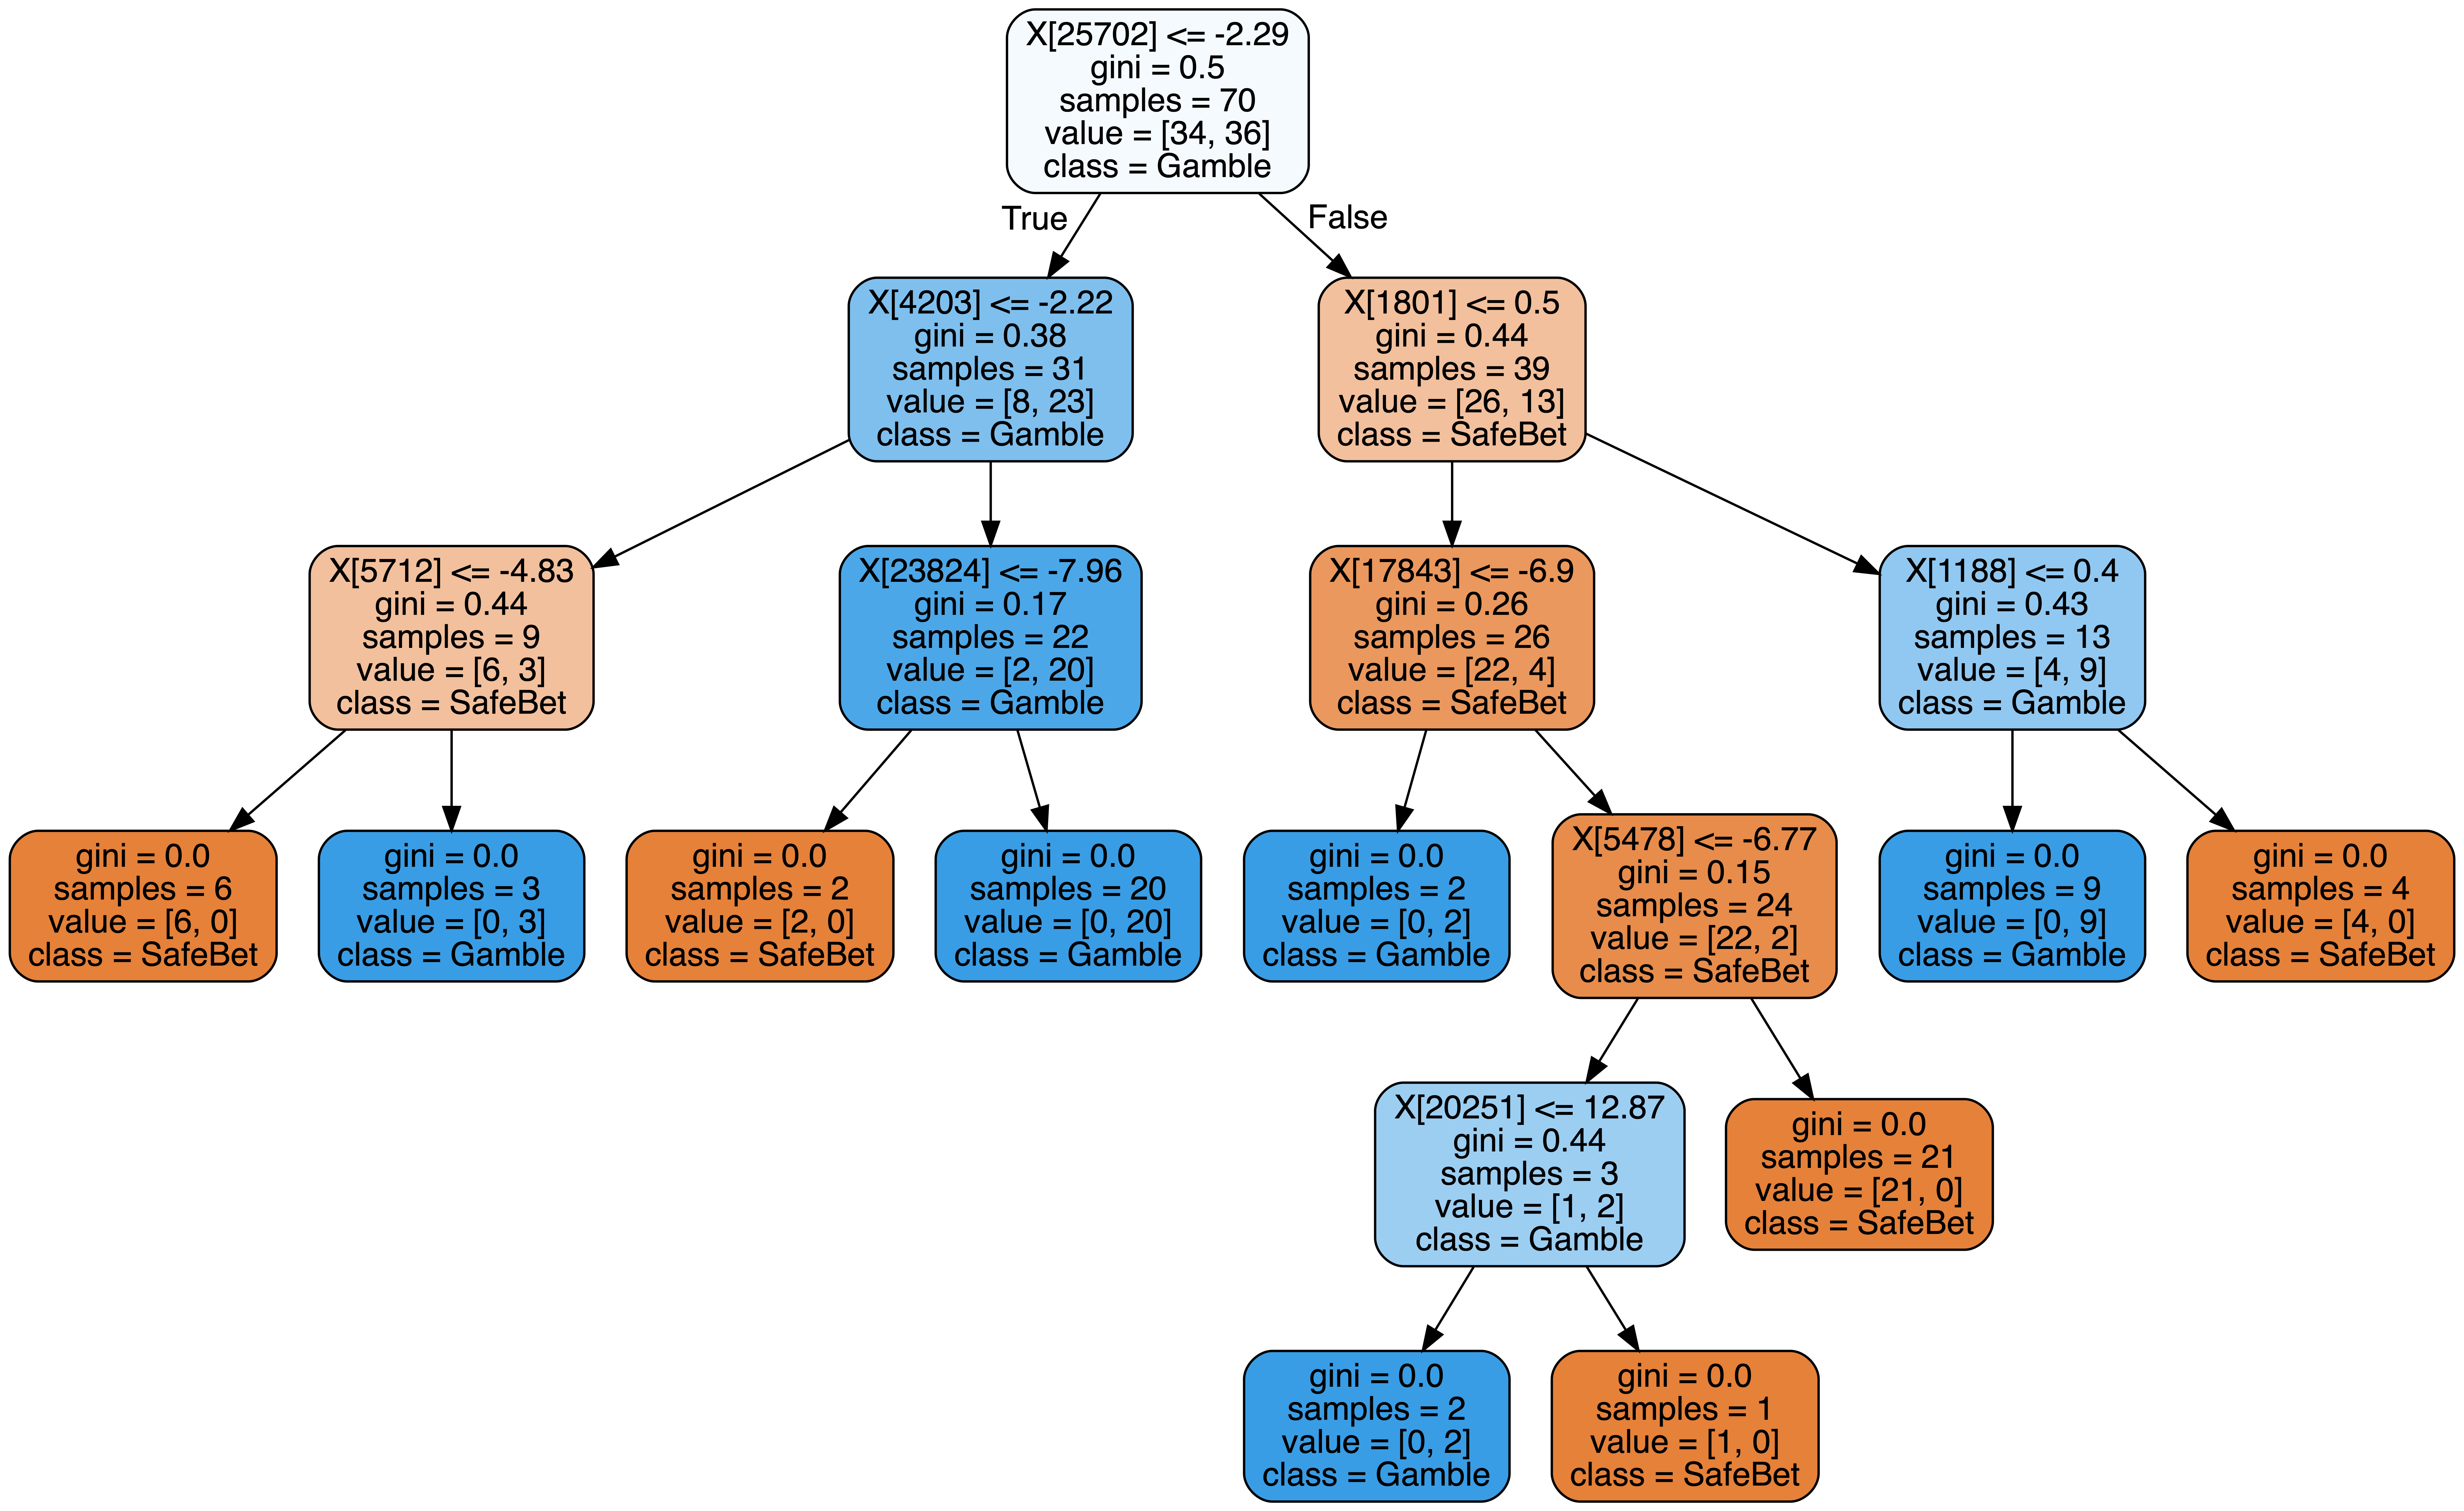
\includegraphics{dt_tree.png}
Random Forest
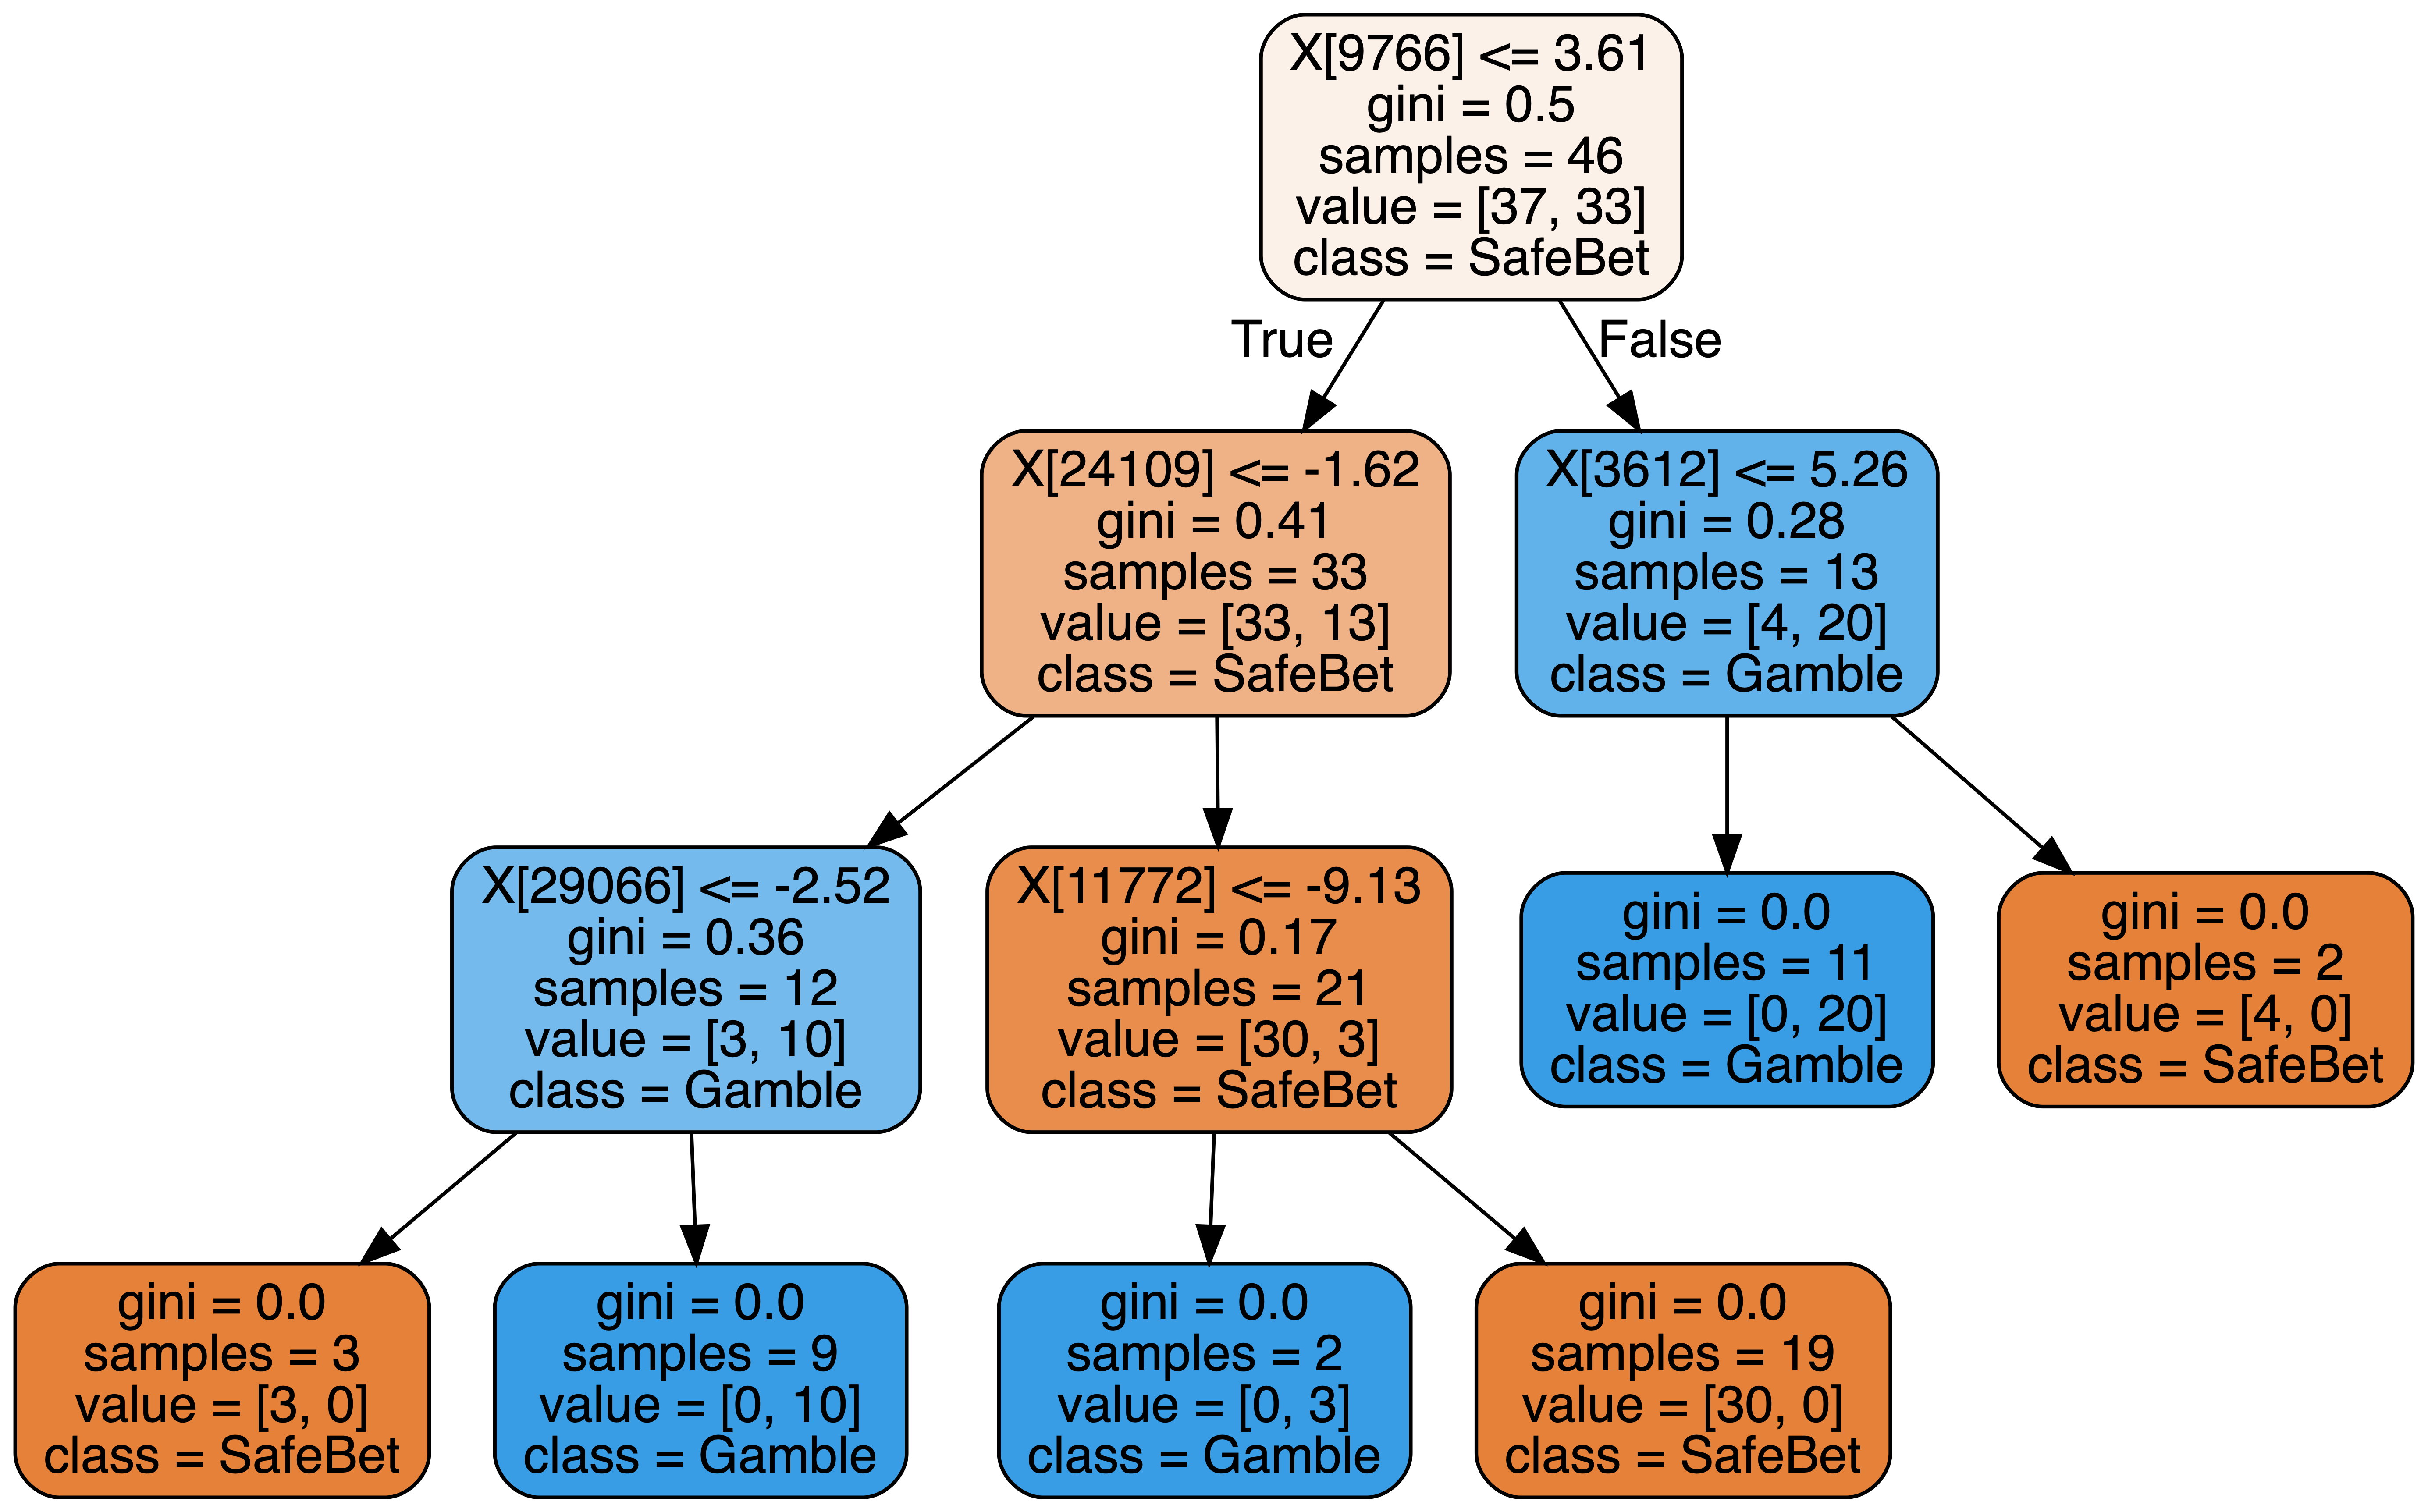
\includegraphics{rand_tree.png}
AdaBoost
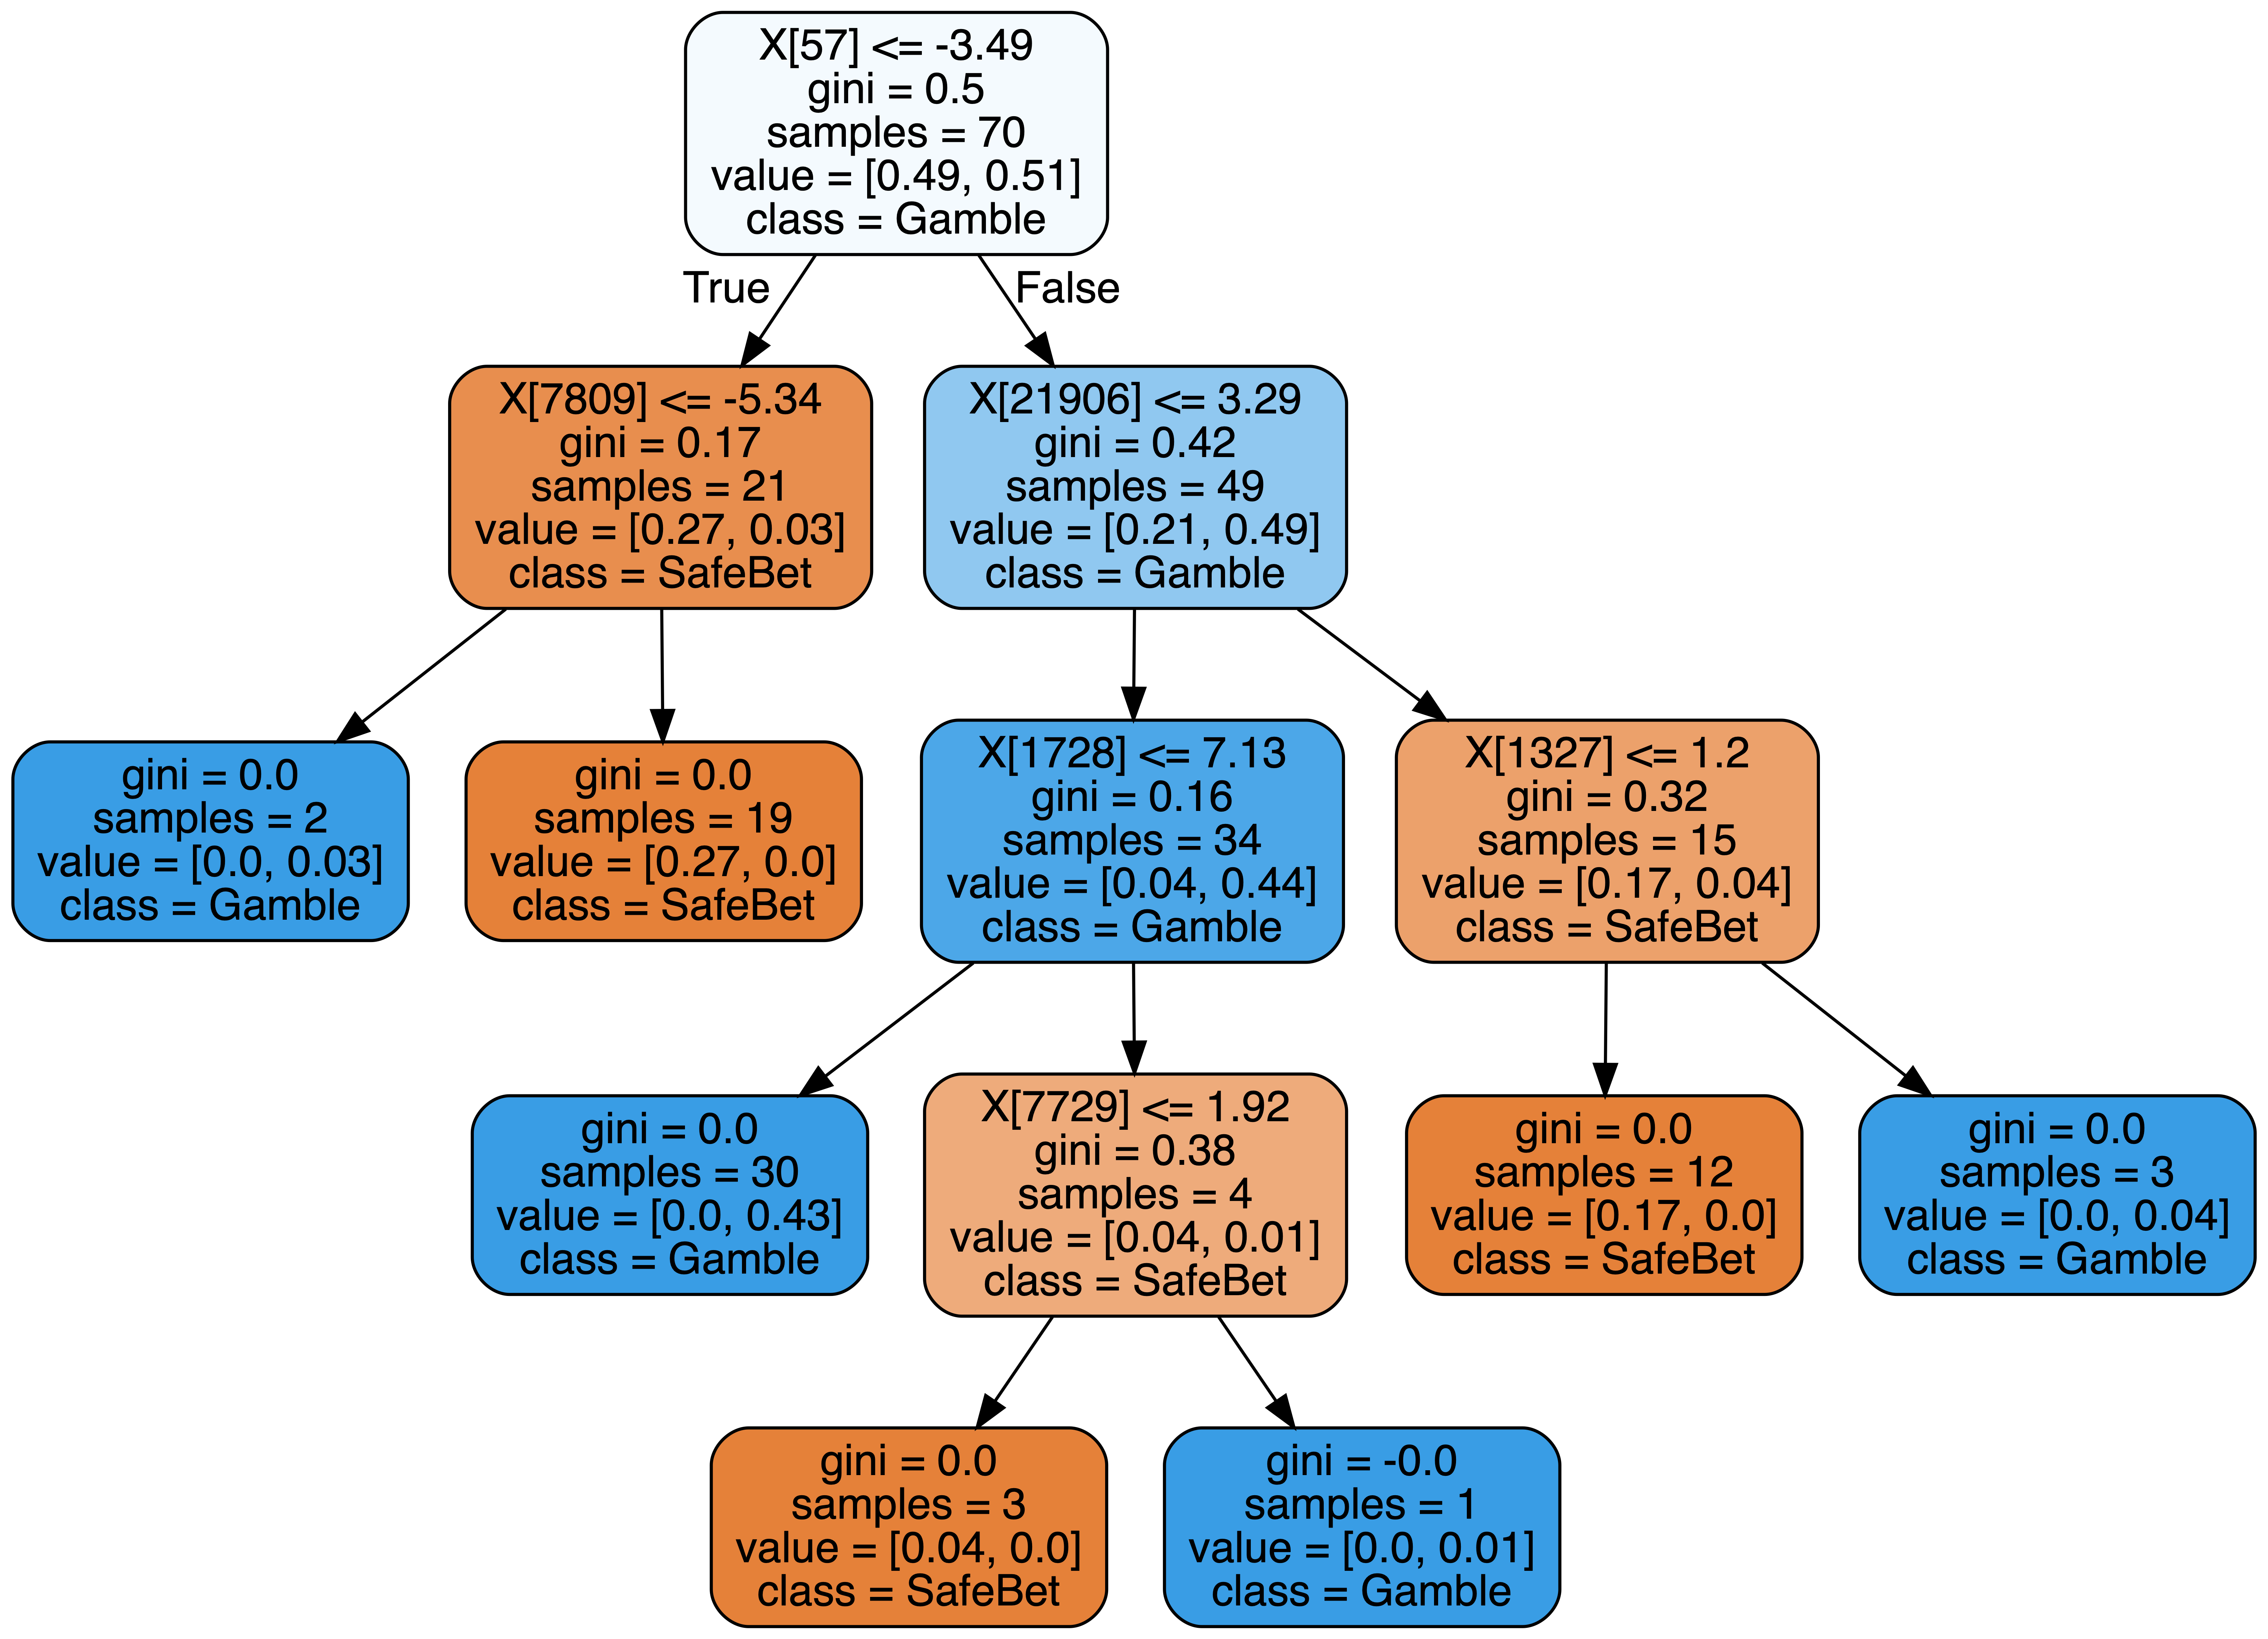
\includegraphics{ada_tree.png}

Above, you can see a graphical representation of the best decision tree
(across all subjects, based on intra-subject accuracy evaluations)
learned by the decision tree classifer, a random decision tree from both
the random forest and AdaBoost ensemble, respectively. To train these
decision tree algorithms, the ECoG recording data for each round that
was in 2 dimensions, i.e., \texttt{(num\_recordings,\ num\_electrodes)},
had to be flatten to a size of
\texttt{num\_recordings\ x\ num\_electrodes}. Hence, the splitting
rules, i.e. \texttt{X{[}21906{]}\textless{}=3.29}, refers to the index
in the flattened recordings array for each round. If more recordings
(i.e.~more \texttt{num\_electrodes}) were available, the splitting rules
would be able to tell us potentially how significant specific ranges of
activity are for a specific recording region. This would give
researchers signifcant aid in understanding how specific areas of the
brain are responsible for making a decision in the brain. However, in
this dataset, only one of the subjects, subject 3, had close to a
reasonable number of electrodes recording activity in the OFC,
specifically 59 electrodes. It should noted that this subject resulted
in highest accuracy in all the classifications above whereas the subject
with the smallest number of electrodes resulted in the least accurate
classifications.

    \hypertarget{conclusiondiscussion}{%
\section{Conclusion/Discussion}\label{conclusiondiscussion}}

    In this notebook, we applied fully-connected and convolutional neural
networks as well decision trees and decision tree ensembles such as
random forest and AdaBoost to the problem of classifying an individual's
action based on their ECoG recording. It should be noted that the number
of electrodes recording OFC neural activity for each subject was shown
to be directly correlated with the performance of each of the models.
That is, the less electrodes were recording a patients neural activity
during the task, the less the accuracy of the classification algorithms
for that patient. This phenomenon is evident in the classification
accuracy for subject 3, who had about 59 electrodes recording data,
which was consistently significantly higher than that of other subjects
in each of the classification schemes. By the end of this notebook, it
is clear that we have fallen short of achieving our initial goal of
finding a machine learning classification algorithm that is able to
predict decisions most of the time (\texttt{\textgreater{}75\%}), even
in the case of a binary classification. It could be argued that the
performance of each of these algorithms could be improved with some
hyperparameter tuning. However, the current accuracy of these models is
significantly low and it is unlikely that any amount of hyperparameter
tuning can bring their accuracy to a level that could be considered
statistically significant compared to random chance. Nonetheless, it
should be noted that the various machine learning classification
algorithms above were just a very small subset of the possible methods
and algorithms that could be applied to this data. More importantly,
these machine learning algorithm require a vast amount of data as input
in order to be able to train accurately. The small number of electrodes
recording neural activity for each patient could very possibly be a
significant factor that affected the performance of our trained models.
Moreover, here, we focused on only using the ECoG recordings as the
basis for predicting the outcome of a patient's decision. One could
extend this approach by incorporating more behavioral information from
the dataset such as the time it took the subject to respond, etc.
However, the goal of this analysis was to find a machine learning model
that based solely on the activation map of the OFC would be able to
predict the decision the patient was going to make.

From the methods tested here, convolutional neural networks and decision
trees showed the greatest potential. These two classification algorithms
provide two very different classification approaches yet similar in the
general idea of feature extraction. If enough data is provided,
convolutional neural networks have the potential to extract very rich
set of features that could help uncover underlying patterns in the OFC
that lead to a specific decision. Similarly, decision trees provided a
set of splitting rules that would allow us to categorize a patient's
brain activity and predict their decision. Working backwards from the
decision, one could uncover the most likely pattern (i.e.~the path
through the decision tree) that leads to a specific decision for an
indvidiual. Overall, with enough accurate brain neural activity
recordings, these approaches have great potential in revealing
previously-obscured patterns in neural activity in the brain's decision
network that could help us understand this decision network better.

    \hypertarget{references}{%
\subsection{References}\label{references}}

    \begin{itemize}
\tightlist
\item
  \textbf{Background}

  \begin{itemize}
  \tightlist
  \item
    {[}1{]} Bolla, K., Eldreth, D., London, E., Kiehl, K., Mouratidis,
    M., Contoreggi, C., . . . Ernst, M. (2003). Orbitofrontal cortex
    dysfunction in abstinent cocaine abusers performing a
    decision-making task. \emph{NeuroImage, 19}(3), 1085-1094.
    doi:10.1016/s1053-8119(03)00113-7
  \item
    {[}2{]} Wallis, J. D. (2007). Orbitofrontal Cortex and Its
    Contribution to Decision-Making. \emph{Annual Review of
    Neuroscience, 30}(1), 31-56.
    doi:10.1146/annurev.neuro.30.051606.094334
  \item
    {[}3{]} Kennerley, S. W., \& Walton, M. E. (2011). Decision making
    and reward in frontal cortex: Complementary evidence from
    neurophysiological and neuropsychological studies. \emph{Behavioral
    Neuroscience, 125}(3), 297-317. doi:10.1037/a0023575
  \item
    {[}4{]} Forbes, E. E., May, J. C., Siegle, G. J., Ladouceur, C. D.,
    Ryan, N. D., Carter, C. S., . . . Dahl, R. E. (2006). Reward-related
    decision-making in pediatric major depressive disorder: An fMRI
    study. \emph{Journal of Child Psychology and Psychiatry, 47}(10),
    1031-1040. doi:10.1111/j.1469-7610.2006.01673.x
  \item
    {[}5{]} Kennerley, S. W., \& Wallis, J. D. (2009). Evaluating
    choices by single neurons in the frontal lobe: Outcome value encoded
    across multiple decision variables. \emph{European Journal of
    Neuroscience, 29}(10), 2061-2073.
    doi:10.1111/j.1460-9568.2009.06743.x
  \item
    {[}6{]} Wallis, J. D. (2011). Cross-species studies of orbitofrontal
    cortex and value-based decision-making. \emph{Nature Neuroscience,
    15}(1), 13-19. doi:10.1038/nn.2956
  \item
    {[}7{]} Walton, M. E., Devlin, J. T., \& Rushworth, M. F. (2004).
    Interactions between decision making and performance monitoring
    within prefrontal cortex. \emph{Nature Neuroscience, 7}(11),
    1259-1265. doi:10.1038/nn1339
  \item
    {[}8{]} Rangel, A., Camerer, C., \& Montague, P. R. (2008). A
    framework for studying the neurobiology of value-based decision
    making. \emph{Nature Reviews Neuroscience, 9}(7), 545-556.
    doi:10.1038/nrn2357
  \item
    {[}9{]} Hsu, M. (2005). Neural Systems Responding to Degrees of
    Uncertainty in Human Decision-Making. \emph{Science, 310}(5754),
    1680-1683. doi:10.1126/science.1115327
  \item
    {[}10{]} Tom, S. M., Fox, C. R., Trepel, C., \& Poldrack, R. A.
    (2007). The Neural Basis of Loss Aversion in Decision-Making Under
    Risk. \emph{Science, 315}(5811), 515-518.
    doi:10.1126/science.1134239
  \item
    {[}11{]} Krain, A. L., Wilson, A. M., Arbuckle, R., Castellanos, F.
    X., \& Milham, M. P. (2006). Distinct neural mechanisms of risk and
    ambiguity: A meta-analysis of decision-making. \emph{NeuroImage,
    32}(1), 477-484. doi:10.1016/j.neuroimage.2006.02.047
  \item
    {[}12{]} Martino, B. D. (2006). Frames, Biases, and Rational
    Decision-Making in the Human Brain. \emph{Science, 313}(5787),
    684-687. doi:10.1126/science.1128356
  \end{itemize}
\item
  \textbf{Methods and dataset description}

  \begin{itemize}
  \tightlist
  \item
    {[}1{]} Asano, E., Juhasz, C., Shah, A., Muzik, O., Chugani, D. C.,
    Shah, J., . . . Chugani, H. T. (2005). Origin and Propagation of
    Epileptic Spasms Delineated on Electrocorticography.
    \emph{Epilepsia, 46}(7), 1086-1097.
    doi:10.1111/j.1528-1167.2005.05205.x
  \end{itemize}
\item
  \textbf{Data Analysis and Results}

  \begin{itemize}
  \tightlist
  \item
    {[}1{]} Bergstra, J., \& Bengio, Y. (2012). Random Search for
    Hyper-Parameter Optimization. \emph{Journal of Machine Learning
    Research, 13}, 281-305. Retrieved December 7, 2018.
  \end{itemize}
\item
  \textbf{Raw data}

  \begin{itemize}
  \tightlist
  \item
    \textbf{OFC-3}Ignacio Saez, Jack Lin, Arjen Stolk, Edward Chang,
    Josef Parvizi, Gerwin Schalk, Robert T. Knight, and Ming Hsu (2018);
    High-frequency activity of human orbitofrontal sites during
    decision-making play. CRCNS.org http://dx.doi.org/10.6080/K0VM49GF
  \end{itemize}
\end{itemize}

    \hypertarget{supplemental-information}{%
\subsection{Supplemental Information}\label{supplemental-information}}

    The \texttt{utils.py} file is added to this submission. All of the
research and early visualizations were done in this notebook and are
included in the checkpoints, if review is needed.


    % Add a bibliography block to the postdoc
    
    
    
    \end{document}
